% content_body.tex
% Gemeinsamer Dokumentinhalt fuer alle Editionen (main.tex, main_kdp_print.tex,
% main_bod_print.tex). Aenderungen an Kapitelreihenfolge, Vorwort oder
% Backmatter nur HIER vornehmen, nicht in den Wrapper-Dateien.
%
% Erwartet, dass der Wrapper vor % content_body.tex
% Gemeinsamer Dokumentinhalt fuer alle Editionen (main.tex, main_kdp_print.tex,
% main_bod_print.tex). Aenderungen an Kapitelreihenfolge, Vorwort oder
% Backmatter nur HIER vornehmen, nicht in den Wrapper-Dateien.
%
% Erwartet, dass der Wrapper vor % content_body.tex
% Gemeinsamer Dokumentinhalt fuer alle Editionen (main.tex, main_kdp_print.tex,
% main_bod_print.tex). Aenderungen an Kapitelreihenfolge, Vorwort oder
% Backmatter nur HIER vornehmen, nicht in den Wrapper-Dateien.
%
% Erwartet, dass der Wrapper vor % content_body.tex
% Gemeinsamer Dokumentinhalt fuer alle Editionen (main.tex, main_kdp_print.tex,
% main_bod_print.tex). Aenderungen an Kapitelreihenfolge, Vorwort oder
% Backmatter nur HIER vornehmen, nicht in den Wrapper-Dateien.
%
% Erwartet, dass der Wrapper vor \input{content_body} optional
% \editionimpressum definiert (Impressum-/ISBN-Text der jeweiligen Ausgabe).
% Ist \editionimpressum nicht definiert, wird ein TODO-Platzhalter gedruckt.

\providecommand{\editionimpressum}{%
    \textbf{TODO: Impressum/ISBN fuer diese Edition eintragen.}\\[1em]
    \textcopyright\ Wolfgang Becker\\
    Alle Rechte vorbehalten.
}

\frontmatter
\maketitle

\cleardoublepage
\thispagestyle{empty}
\vspace*{\fill}
\noindent
\editionimpressum
\vspace*{\fill}
\clearpage

\tableofcontents

\chapter*{Vorwort}
Dieses Lehrbuch richtet sich an Einsteiger ohne Vorkenntnisse in SysML v2, MBSE oder ROS2.
Das Ziel ist nicht, alle Spezialfälle der Modellierungstheorie abzudecken. Das Ziel ist, ein funktionierendes Verständnis aufzubauen:
Was ist ein Systemmodell? Wie beschreibt man Anforderungen? Wie entsteht daraus eine Architektur? Und wie lässt sich diese Architektur auf ein ROS2-Robotiksystem übertragen?

Als durchgängiges Beispiel dient ein autonomer Indoor-Roboter. Der Roboter soll Hindernisse erkennen, Räume kartieren, Ziele anfahren, Personen erkennen und seinen Akkustand überwachen.
Das Beispiel ist klein genug für den Einstieg, aber realistisch genug, um die wichtigsten Ideen von Model-Based Systems Engineering sichtbar zu machen.

Alle SysML-v2-Codebeispiele in diesem Buch wurden mit dem Syside Editor geprüft (Version 0.10.2, geprüft am 07.07.2026). Da sich SysML v2 und die zugehörigen Werkzeuge derzeit noch kontinuierlich weiterentwickeln, kann es bei abweichenden Werkzeugversionen zu kleinen Syntaxunterschieden kommen, etwa bei der Schreibweise von \texttt{verify ... by}. Prüfen Sie Codebeispiele im Zweifel gegen Ihre installierte Werkzeugversion.

\mainmatter

\input{chapters/01_systems_engineering}
\input{chapters/02_mbse}
\input{chapters/03_sysml_grundlagen}
\input{chapters/04_sysml_v2_werkzeuge}
\input{chapters/05_praxisprojekt}
\input{chapters/06_anforderungen}
\input{chapters/07_stakeholder_use_cases}
\input{chapters/08_bdd}
\input{chapters/09_ibd}
\input{chapters/10_schnittstellen}
\input{chapters/11_activity_diagrams}
\input{chapters/12_state_machines}
\input{chapters/13_parametrik}
\input{chapters/14_ros2_grundlagen}
\input{chapters/15_ros2_architektur}
\input{chapters/16_sysml_ros2_mapping}
\input{chapters/17_ros2_python}
\input{chapters/18_ml_integration}
\input{chapters/19_tests_verifikation}
\input{chapters/20_traceability}
\input{chapters/21_abschlussprojekt}
\input{chapters/22_ausblick}

\backmatter
\glsaddall
\printglossary[type=\acronymtype,title=Abkürzungsverzeichnis]
\printglossary[title=Glossar]
\bibliographystyle{plain}
\bibliography{references}

\listoffigures

\printindex
 optional
% \editionimpressum definiert (Impressum-/ISBN-Text der jeweiligen Ausgabe).
% Ist \editionimpressum nicht definiert, wird ein TODO-Platzhalter gedruckt.

\providecommand{\editionimpressum}{%
    \textbf{TODO: Impressum/ISBN fuer diese Edition eintragen.}\\[1em]
    \textcopyright\ Wolfgang Becker\\
    Alle Rechte vorbehalten.
}

\frontmatter
\maketitle

\cleardoublepage
\thispagestyle{empty}
\vspace*{\fill}
\noindent
\editionimpressum
\vspace*{\fill}
\clearpage

\tableofcontents

\chapter*{Vorwort}
Dieses Lehrbuch richtet sich an Einsteiger ohne Vorkenntnisse in SysML v2, MBSE oder ROS2.
Das Ziel ist nicht, alle Spezialfälle der Modellierungstheorie abzudecken. Das Ziel ist, ein funktionierendes Verständnis aufzubauen:
Was ist ein Systemmodell? Wie beschreibt man Anforderungen? Wie entsteht daraus eine Architektur? Und wie lässt sich diese Architektur auf ein ROS2-Robotiksystem übertragen?

Als durchgängiges Beispiel dient ein autonomer Indoor-Roboter. Der Roboter soll Hindernisse erkennen, Räume kartieren, Ziele anfahren, Personen erkennen und seinen Akkustand überwachen.
Das Beispiel ist klein genug für den Einstieg, aber realistisch genug, um die wichtigsten Ideen von Model-Based Systems Engineering sichtbar zu machen.

Alle SysML-v2-Codebeispiele in diesem Buch wurden mit dem Syside Editor geprüft (Version 0.10.2, geprüft am 07.07.2026). Da sich SysML v2 und die zugehörigen Werkzeuge derzeit noch kontinuierlich weiterentwickeln, kann es bei abweichenden Werkzeugversionen zu kleinen Syntaxunterschieden kommen, etwa bei der Schreibweise von \texttt{verify ... by}. Prüfen Sie Codebeispiele im Zweifel gegen Ihre installierte Werkzeugversion.

\mainmatter

\chapter{Systems Engineering verstehen}

\begin{lernziele}
Nach diesem Kapitel können Sie erklären, was ein System ist, warum Systems Engineering bei komplexen Produkten notwendig wird und warum ein autonomer Roboter mehr ist als eine Sammlung einzelner Bauteile.
\end{lernziele}

\section{Was ist ein System?}
Ein System ist eine Menge von Elementen, die zusammenwirken, um einen Zweck zu erfüllen. Ein autonomer Indoor-Roboter besteht zum Beispiel aus Sensoren, Rechner, Software, Batterie, Motoren, Rädern, Gehäuse und Benutzerschnittstellen. Entscheidend ist nicht nur, dass diese Elemente existieren. Entscheidend ist, dass sie zusammen funktionieren.

Ein einzelner Lidar-Sensor macht noch keinen autonomen Roboter. Erst wenn Sensordaten verarbeitet, in eine Karte eingebaut, mit einer Navigation verknüpft und in Motorbefehle übersetzt werden, entsteht ein Systemverhalten.

\section{Warum Systems Engineering?}
In einfachen Projekten reicht es oft aus, direkt mit der Umsetzung zu beginnen. Bei komplexeren technischen Systemen führt das schnell zu Problemen. Eine Änderung an einer Komponente kann viele andere Bereiche beeinflussen. Eine stärkere Kamera kann zum Beispiel mehr Rechenleistung benötigen, mehr Strom verbrauchen und andere Treiber voraussetzen.

Systems Engineering hilft dabei, solche Abhängigkeiten sichtbar zu machen. Es zwingt nicht zu Bürokratie, sondern zu Klarheit: Was soll das System leisten? Welche Komponenten sind beteiligt? Welche Schnittstellen gibt es? Wie wird geprüft, ob das System funktioniert?

\begin{praxisbox}
Beim autonomen Indoor-Roboter reicht die Aussage \enquote{Der Roboter soll fahren} nicht aus. Wir müssen wissen, wo er fahren soll, wie schnell er fahren darf, welche Hindernisse erkannt werden müssen, welche Sensoren eingesetzt werden und was bei niedrigem Akkustand passiert.
\end{praxisbox}

\section{Systemgrenze}
Eine wichtige Entscheidung ist die Systemgrenze. Sie legt fest, was zum betrachteten System gehört und was nur Teil der Umgebung ist. Beim Indoor-Roboter kann die Ladestation zum System gehören oder als externes System modelliert werden. Beide Entscheidungen sind möglich, aber sie müssen bewusst getroffen werden.

\section{Stakeholder}
Stakeholder sind Personen oder Organisationen, die Anforderungen an das System haben. Beim Roboter sind das zum Beispiel Nutzer, Betreiber, Wartungspersonal, Entwickler und möglicherweise Sicherheitsbeauftragte. Unterschiedliche Stakeholder haben unterschiedliche Interessen. Nutzer wollen einfache Bedienung. Wartungspersonal will Diagnosemöglichkeiten. Entwickler wollen klare Schnittstellen.

\section{Typische Fehler am Anfang}
Ein häufiger Fehler besteht darin, sofort Komponenten zu zeichnen. Das wirkt produktiv, überspringt aber die Frage, warum diese Komponenten überhaupt gebraucht werden. Ein anderer Fehler ist, Anforderungen zu allgemein zu formulieren. \enquote{Der Roboter soll zuverlässig sein} klingt gut, ist aber kaum testbar.

\begin{uebungbox}
Beschreiben Sie den autonomen Indoor-Roboter in fünf Sätzen. Markieren Sie anschließend, welche Wörter Funktionen, Komponenten, Stakeholder oder Randbedingungen beschreiben.
\end{uebungbox}

\chapter{Einführung in Model-Based Systems Engineering}

\begin{lernziele}
Nach diesem Kapitel verstehen Sie den Unterschied zwischen dokumentenzentrierter Entwicklung und modellbasierter Entwicklung. Sie können erklären, warum ein zentrales Modell bei komplexen Projekten nützlich ist.
\end{lernziele}

\section{Dokumentenzentrierte Entwicklung}
In vielen Projekten liegen Informationen verstreut vor: Anforderungen in Excel, Architektur in PowerPoint, Schnittstellen in Word, Aufgaben in Jira und Code in Git. Das funktioniert eine Zeit lang, wird aber unübersichtlich. Sobald Änderungen auftreten, ist unklar, welche Dokumente angepasst werden müssen.

\section{Modellbasierte Entwicklung}
\gls{mbse} verwendet ein Modell als zentrale Informationsquelle. Dieses Modell enthält Anforderungen, Struktur, Verhalten, Schnittstellen und Tests. Das Modell ersetzt nicht den Code und nicht jede technische Spezifikation. Es verbindet aber die wichtigsten Informationen.

\section{Vorteile von MBSE}
Die wichtigsten Vorteile sind Nachvollziehbarkeit, Konsistenz und bessere Kommunikation. Ein Entwickler sieht, welche Anforderung eine Komponente erfüllt. Ein Tester sieht, welcher Test zu welcher Anforderung gehört. Ein Projektleiter erkennt, welche Teile von einer Änderung betroffen sind.

\begin{hinweisbox}
MBSE bedeutet nicht, dass jedes Detail modelliert werden muss. Ein gutes Modell ist so detailliert wie nötig und so einfach wie möglich.
\end{hinweisbox}

\section{MBSE im Roboterprojekt}
Für unseren Roboter modellieren wir Anforderungen, Systemstruktur, Datenflüsse, Verhalten, ROS2-Komponenten und Tests. Damit entsteht eine Kette von der Idee bis zur Umsetzung.

\begin{center}
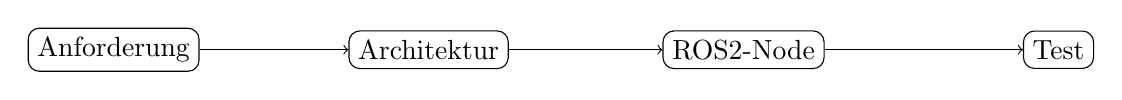
\begin{tikzpicture}[node distance=1.6cm]
\node (req) [draw, rounded corners] {Anforderung};
\node (arch) [draw, rounded corners, right of=req, xshift=2.4cm] {Architektur};
\node (impl) [draw, rounded corners, right of=arch, xshift=2.4cm] {ROS2-Node};
\node (test) [draw, rounded corners, right of=impl, xshift=2.4cm] {Test};
\draw[->] (req) -- (arch);
\draw[->] (arch) -- (impl);
\draw[->] (impl) -- (test);
\end{tikzpicture}
\end{center}

\section{Grenzen von MBSE}
MBSE löst keine schlechten technischen Entscheidungen. Ein Modell kann falsch, veraltet oder unnötig kompliziert sein. Der Nutzen entsteht nur, wenn das Modell gepflegt wird und echte Entscheidungen unterstützt.

\begin{uebungbox}
Erstellen Sie eine Tabelle mit drei Spalten: Information, klassischer Speicherort und Speicherort im MBSE-Modell. Tragen Sie Anforderungen, Schnittstellen, Tests und ROS2-Nodes ein.
\end{uebungbox}

\chapter{SysML-Grundlagen}

\begin{lernziele}
Nach diesem Kapitel kennen Sie die wichtigsten SysML-Diagrammtypen und wissen, wofür sie eingesetzt werden.
\end{lernziele}

\section{Was ist SysML?}
\gls{sysml} steht für Systems Modeling Language. Die Sprache wurde entwickelt, um technische Systeme modellieren zu können. Sie basiert auf UML, ist aber stärker auf Systeme aus Hardware, Software, Menschen, Prozessen und physikalischen Zusammenhängen ausgerichtet.

\section{Diagrammtypen}
Für den Einstieg sind sechs Diagrammtypen besonders wichtig.

\subsection{Requirement Diagram}
Das Requirement Diagram beschreibt Anforderungen und ihre Beziehungen. Es zeigt, welche Anforderungen voneinander abhängen und welche Elemente sie erfüllen oder verifizieren.

\subsection{Block Definition Diagram}
Das \gls{bdd} beschreibt die Systemstruktur auf einer eher abstrakten Ebene. Es zeigt Blöcke und ihre Beziehungen.

\subsection{Internal Block Diagram}
Das \gls{ibd} zeigt die innere Struktur eines Blocks. Es zeigt Teile, Ports und Verbindungen.

\subsection{Activity Diagram}
Aktivitätsdiagramme beschreiben Abläufe. Sie eignen sich für Prozesse, Algorithmen und Betriebsabläufe.

\subsection{State Machine Diagram}
Zustandsdiagramme beschreiben Zustände und Übergänge. Sie sind besonders nützlich für Systeme mit klaren Betriebsmodi.

\subsection{Parametric Diagram}
Parametrische Diagramme beschreiben mathematische Beziehungen, zum Beispiel Energieverbrauch oder Reichweite.

\section{Nicht alles gleichzeitig lernen}
Einsteiger sollten nicht versuchen, sofort jedes Diagramm perfekt zu beherrschen. Der sinnvolle Einstieg lautet: Anforderungen, BDD, IBD, Aktivitätsdiagramm und Zustandsdiagramm. Parametrik kann später folgen.

\begin{praxisbox}
Für den Indoor-Roboter beginnen wir mit Anforderungen und Struktur. Erst wenn klar ist, was der Roboter können soll und aus welchen Hauptsystemen er besteht, modellieren wir Verhalten und technische Details.
\end{praxisbox}

\section{Modell statt Bild}
Ein SysML-Diagramm ist nur eine Sicht auf ein Modell. Das ist wichtig: Wenn ein Block in mehreren Diagrammen erscheint, ist es derselbe Block. Wird der Name geändert, sollte sich die Änderung überall widerspiegeln. Gute Modellierungswerkzeuge speichern also nicht nur Zeichnungen, sondern Modellinformationen.

\begin{uebungbox}
Ordnen Sie folgende Fragen einem Diagrammtyp zu: Was muss das System leisten? Aus welchen Teilen besteht es? Welche Daten fließen zwischen Komponenten? Welche Zustände kann der Roboter haben?
\end{uebungbox}

\chapter{Werkzeuge für SysML v2 einrichten}

\begin{lernziele}
Nach diesem Kapitel können Sie erklären, warum dieses Lehrbuch eine textuelle SysML-v2-Arbeitsweise verwendet. Sie können ein einfaches Projekt in VS Code mit dem Syside Editor anlegen, SysML-v2-Dateien strukturieren und grafische Sichten als Ergänzung einordnen. Außerdem verstehen Sie, warum ein Werkzeug fachliches Modellieren unterstützt, aber nicht ersetzt.
\end{lernziele}

\section{Einleitung}
SysML v2 kann grafisch und textuell verwendet werden. Für dieses Lehrbuch steht die textuelle Notation im Vordergrund. Das passt gut zu modernen Entwicklungsabläufen: Modelle liegen in Dateien, können versioniert, verglichen, überprüft und gemeinsam mit Code gepflegt werden.

Als kostenloser Einstieg eignet sich der Syside Editor für VS Code. Er unterstützt SysML-v2-Dateien mit Syntaxhervorhebung, Autovervollständigung, Formatierung, Gliederung und Validierung. Für grafische Sichten kann zusätzlich Eclipse SysON genutzt werden. SysON ist ein webbasiertes Open-Source-Werkzeug für SysML-v2-Modelle.

\begin{hinweisbox}
Ein Werkzeug löst keine Modellierungsaufgabe automatisch. Es hilft beim Schreiben, Prüfen und Anzeigen des Modells. Die fachliche Entscheidung bleibt Ihre Aufgabe: Welche Elemente gibt es? Welche Beziehungen sind wichtig? Welche Anforderungen müssen nachverfolgbar sein?
\end{hinweisbox}

\section{Warum textuelle Modellierung?}
Viele Einsteiger erwarten bei SysML zuerst Diagramme. Diagramme bleiben wichtig, aber SysML v2 macht den Modellinhalt stärker als präzisen Text zugänglich. Ein Modell kann dadurch ähnlich behandelt werden wie Quellcode.

Textuelle Modellierung hat mehrere Vorteile:

\begin{itemize}
    \item Modelle lassen sich in Git versionieren.
    \item Änderungen sind als Textvergleich sichtbar.
    \item Beispiele können direkt im Lehrbuch gezeigt werden.
    \item Modellteile können leichter wiederverwendet werden.
    \item Validierung und Automatisierung werden einfacher.
    \item ROS2-Code und SysML-v2-Modell können im selben Projekt liegen.
\end{itemize}

Das bedeutet nicht, dass Diagramme unwichtig werden. Diagramme sind weiterhin wertvolle Sichten. Der Unterschied ist: Das Modell entsteht nicht nur durch Zeichnen, sondern durch präzise definierte Modellelemente.

\section{Empfohlene Werkzeugkette}
Für dieses Lehrbuch verwenden wir eine einfache Werkzeugkette:

\begin{itemize}
    \item VS Code als Editor
    \item Syside Editor als SysML-v2-Erweiterung
    \item Git für Versionsverwaltung
    \item optional Eclipse SysON für grafische Sichten
    \item optional das SysML-v2-Pilotprojekt als Referenz für fortgeschrittene Experimente
\end{itemize}

Diese Auswahl ist bewusst pragmatisch. Sie ist kostenlos zugänglich, passt zu textueller Modellierung und überfordert Einsteiger weniger als große industrielle Modellierungsumgebungen.

\section{Projekt anlegen}
Für das Lehrbuch verwenden wir ein Projekt mit dem Namen \texttt{AutonomousIndoorRobot}. Der Name ist bewusst englisch, weil spätere ROS2-Pakete, Nodes und Topics ebenfalls englische technische Bezeichnungen verwenden. Die erklärenden Texte im Modell können trotzdem deutsch sein.

Eine einfache Projektstruktur kann so aussehen:

\begin{verbatim}
AutonomousIndoorRobot/
  model/
    00_overview.sysml
    01_context.sysml
    02_requirements.sysml
    03_structure.sysml
    04_behavior.sysml
    05_interfaces.sysml
    06_tests.sysml
    07_ros2_mapping.sysml
  code/
    status_node.py
    battery_monitor_node.py
  docs/
    decisions.md
\end{verbatim}

Die Dateien im Ordner \texttt{model} enthalten das SysML-v2-Modell. Der Ordner \texttt{code} enthält spätere ROS2-Beispiele. Der Ordner \texttt{docs} kann kurze Architekturentscheidungen aufnehmen.

\section{Erste SysML-v2-Datei}
Eine erste Datei \texttt{00\_overview.sysml} kann den Projektrahmen beschreiben:

\begin{lstlisting}
package AutonomousIndoorRobot {
  doc
  /* Ein Lernmodell für einen autonomen Indoor-Roboter.
     Das Modell verbindet Anforderungen, Struktur, Verhalten,
     Schnittstellen, ROS2-Mapping und Tests. */

  part def Robot;
}
\end{lstlisting}

Dieses Beispiel ist noch sehr klein. Es zeigt aber bereits eine wichtige Idee: Das System wird nicht als loses Bild begonnen, sondern als benannter Modellraum mit einem ersten Systemelement.

\section{Empfohlene Modellstruktur}
Die Modellstruktur orientiert sich an den wichtigsten Fragen des Projekts:

\begin{itemize}
    \item \texttt{00\_overview.sysml}: Ziel, Umfang und Systemgrenze
    \item \texttt{01\_context.sysml}: Stakeholder, externe Systeme und Umgebung
    \item \texttt{02\_requirements.sysml}: Anforderungen und Beziehungen
    \item \texttt{03\_structure.sysml}: Systemteile, Subsysteme und Komponenten
    \item \texttt{04\_behavior.sysml}: Aktionen, Abläufe und Zustände
    \item \texttt{05\_interfaces.sysml}: Ports, Verbindungen und Datenflüsse
    \item \texttt{06\_tests.sysml}: Testfälle und Verifikation
    \item \texttt{07\_ros2\_mapping.sysml}: Zuordnung zu ROS2-Nodes, Topics, Services und Actions
\end{itemize}

Diese Struktur ist bewusst schlicht. Sie trennt die wichtigsten Modellbereiche, ohne schon zu Beginn ein kompliziertes Metamodell einzuführen.

\section{Namenskonventionen}
Klare Namen machen Modelle lesbar. Für dieses Lehrbuch verwenden wir einfache Regeln:

\begin{itemize}
    \item Packages: \texttt{AutonomousIndoorRobot}
    \item Part Definitions: \texttt{Robot}, \texttt{BatterySystem}, \texttt{NavigationSystem}
    \item Parts: \texttt{batterySystem}, \texttt{navigationSystem}
    \item Actions: \texttt{MonitorBattery}, \texttt{NavigateToGoal}
    \item Requirements: \texttt{REQ\_DetectObstacles}, \texttt{REQ\_ReturnToDock}
    \item Testfälle: \texttt{TC\_BatteryLowReturn}
    \item ROS2-Nodes: \texttt{battery\_monitor\_node}
    \item Topics: \texttt{/battery\_state}, \texttt{/cmd\_vel}
\end{itemize}

Vermeiden Sie wechselnde Namen für dasselbe Element. Wenn ein Element einmal \texttt{BatterySystem} heißt, sollte es nicht an anderer Stelle \texttt{PowerModule} genannt werden, außer Sie modellieren bewusst unterschiedliche Dinge.

\section{Grafische Sichten}
Grafische Sichten sind besonders hilfreich, wenn ein Team schnell über Struktur oder Schnittstellen sprechen möchte. In SysML v2 sollte man sie als Darstellung des Modells verstehen, nicht als Ersatz für das Modell.

Eclipse SysON kann für solche Sichten interessant sein. Es ist besonders dann nützlich, wenn Sie aus dem textuellen Modell heraus Struktur-, Verbindungs- oder Anforderungssichten visualisieren wollen. Für den Einstieg in diesem Buch reicht es aber, zunächst die textuelle Notation sauber zu verstehen.

\section{Typische Anfängerfehler}
\subsection{Text wie Programmcode ohne Bedeutung schreiben}
SysML-v2-Text sieht teilweise wie Code aus. Trotzdem modellieren Sie kein Programm, sondern ein System. Fragen Sie bei jedem Element: Welche fachliche Aussage steckt dahinter?

\subsection{Zu früh zu viele Dateien anlegen}
Eine klare Struktur hilft, aber zu viele leere Dateien machen den Einstieg schwer. Beginnen Sie mit Überblick, Anforderungen und Struktur. Verhalten, Tests und Mapping können anschließend wachsen.

\subsection{Diagramme als Wahrheit behandeln}
Ein Diagramm zeigt nur eine Sicht. Die eigentliche Wahrheit liegt im Modell und seinen Beziehungen. Wenn Diagramm und Modell auseinanderlaufen, muss das Modell geklärt werden.

\subsection{Werkzeugvalidierung mit Modellqualität verwechseln}
Ein syntaktisch gültiges Modell kann fachlich trotzdem schlecht sein. Validierung findet Schreibfehler und Regelverstöße, aber keine unklare Systemgrenze oder fehlende Sicherheitsanforderung.

\section{Zusammenfassung}
Dieses Lehrbuch verwendet SysML v2 textuell und einsteigerfreundlich. VS Code mit dem Syside Editor ist die empfohlene kostenlose Arbeitsumgebung. Eclipse SysON kann grafische Sichten ergänzen. Entscheidend bleibt aber nicht das Werkzeug, sondern ein verständliches, konsistentes und nachverfolgbares Modell.

\section{Kontrollfragen}
\begin{enumerate}
    \item Warum eignet sich textuelle Modellierung gut für SysML v2?
    \item Welche Rolle spielt der Syside Editor in diesem Lehrbuch?
    \item Warum sind grafische Sichten trotzdem nützlich?
    \item Welche Dateien enthält die empfohlene Modellstruktur?
    \item Warum sollten Modellelemente einheitlich benannt werden?
    \item Warum ersetzt Werkzeugvalidierung keine fachliche Modellprüfung?
\end{enumerate}

\section{Übungen}
\begin{uebungbox}
\textbf{Übung 1: Projektstruktur anlegen}\\
Legen Sie die empfohlene Ordnerstruktur für \texttt{AutonomousIndoorRobot} an. Erstellen Sie eine Datei \texttt{00\_overview.sysml} und beschreiben Sie Ziel, Umfang und Systemgrenze des Roboterprojekts.
\end{uebungbox}

\begin{uebungbox}
\textbf{Übung 2: Namensregeln anwenden}\\
Formulieren Sie Namen für fünf Anforderungen, drei Testfälle, fünf Part Definitions und vier ROS2-Topics. Achten Sie auf einheitliche Schreibweise.
\end{uebungbox}

\begin{uebungbox}
\textbf{Übung 3: Sicht statt Wahrheit}\\
Beschreiben Sie in drei Sätzen, warum ein Diagramm in SysML v2 nur eine Sicht auf das Modell ist.
\end{uebungbox}

\section{Literaturhinweise}
Für die praktische Arbeit mit SysML v2 sind die Dokumentation des Syside Editors, das Eclipse-SysON-Projekt und das SysML-v2-Pilotprojekt hilfreich \cite{syside,syson,sysmlv2pilot}. Für die fachliche Einordnung bleiben klassische SysML- und MBSE-Grundlagen nützlich, müssen aber bewusst auf SysML v2 übertragen werden.

\chapter{Das Praxisprojekt: Autonomer Indoor-Roboter}

\begin{lernziele}
Nach diesem Kapitel kennen Sie das Beispielsystem, seine Hauptfunktionen und die wichtigsten Randbedingungen.
\end{lernziele}

\section{Ziel des Systems}
Der autonome Indoor-Roboter soll sich in Innenräumen bewegen, Hindernisse erkennen, Personen erkennen, Ziele anfahren und bei niedrigem Akkustand zur Ladestation zurückkehren.

\section{Warum dieses Beispiel?}
Das Beispiel verbindet mehrere typische Bereiche moderner Systementwicklung: Sensorik, Aktorik, Software, Datenverarbeitung, Robotik, künstliche Intelligenz und Tests. Es ist komplex genug, damit SysML Sinn ergibt, aber nicht so groß, dass Einsteiger den Überblick verlieren.

\section{Hauptfunktionen}
\begin{itemize}
\item Umgebung erfassen
\item Karte erstellen oder laden
\item Position bestimmen
\item Navigationsziel empfangen
\item Pfad planen
\item Hindernissen ausweichen
\item Personen erkennen
\item Batterie überwachen
\item Ladestation anfahren
\end{itemize}

\section{Systemkontext}
Der Roboter interagiert mit Nutzern, Räumen, Hindernissen, Ladestation und Wartungspersonal. Diese externen Elemente gehören nicht alle zwingend zum System, beeinflussen aber Anforderungen und Schnittstellen.

\section{Annahmen}
Für dieses Lehrbuch nehmen wir an, dass der Roboter mit Kamera, Lidar, mobilem Rechner, Motorcontroller und Batterie ausgestattet ist. Als Softwarebasis verwenden wir ROS2. Für die Personenerkennung wird später ein ML-Modell eingebunden.

\begin{hinweisbox}
Das Projekt ist didaktisch vereinfacht. Ein echter sicherheitskritischer Roboter würde zusätzliche Sicherheitsanalysen, Normenbetrachtungen und Zulassungsprozesse benötigen.
\end{hinweisbox}

\begin{uebungbox}
Zeichnen Sie eine einfache Kontextskizze: Roboter in der Mitte, außen Nutzer, Hindernis, Ladestation, Raum und Wartungstechniker.
\end{uebungbox}

\chapter{Anforderungen modellieren}

\begin{lernziele}
Nach diesem Kapitel können Sie Anforderungen verständlich, eindeutig und prüfbar formulieren. Sie können Anforderungen nummerieren, strukturieren, in funktionale und nicht-funktionale Anforderungen unterscheiden und mit SysML-Beziehungen verbinden. Außerdem verstehen Sie, wie Anforderungen im Roboterprojekt von Stakeholderbedürfnissen bis zu Testfällen nachverfolgt werden.
\end{lernziele}

\section{Einleitung}
Anforderungen sind eine der wichtigsten Grundlagen eines Systemmodells. Sie beschreiben, was das System leisten muss und unter welchen Bedingungen es dies tun soll. Ohne gute Anforderungen ist unklar, welche Architektur sinnvoll ist und woran der Projekterfolg gemessen wird.

Beim autonomen Indoor-Roboter klingen viele Wünsche zunächst einfach: Der Roboter soll sicher fahren, Hindernisse erkennen, Personen erkennen, lange genug fahren und leicht bedienbar sein. Für die Entwicklung reicht das nicht. Solche Wünsche müssen in Anforderungen übersetzt werden, die eindeutig und später überprüfbar sind.

\section{Was ist eine gute Anforderung?}
Eine gute Anforderung ist:

\begin{itemize}
    \item verständlich
    \item eindeutig
    \item notwendig
    \item realistisch
    \item prüfbar
    \item möglichst lösungsneutral
\end{itemize}

\enquote{Der Roboter soll gut navigieren} ist keine gute Anforderung. Was bedeutet \enquote{gut}? Schnell? Genau? Sicher? Ohne Kollision? In unbekannten Räumen? Eine bessere Formulierung lautet:

\begin{quote}
Der Roboter muss in einem bekannten Innenraum ein ausgewähltes Ziel autonom anfahren und dabei statische Hindernisse im Fahrweg vermeiden.
\end{quote}

Auch diese Anforderung kann später noch präziser werden, aber sie ist deutlich verständlicher.

\section{Vom Bedürfnis zur Anforderung}
Stakeholder äußern häufig Bedürfnisse. Diese Bedürfnisse sind wichtig, aber noch keine technischen Anforderungen.

\begin{center}
\begin{tabular}{p{0.38\textwidth}p{0.50\textwidth}}
\toprule
\textbf{Bedürfnis} & \textbf{Mögliche Anforderung} \\
\midrule
Der Roboter soll niemanden gefährden. & Der Roboter muss bei einem Hindernis im Abstand von 0,5 m seine Geschwindigkeit reduzieren und bei 0,2 m stoppen. \\
Der Roboter soll einfach bedienbar sein. & Ein Transportauftrag muss mit höchstens drei Eingaben gestartet werden können. \\
Der Roboter soll nicht liegen bleiben. & Der Roboter muss bei niedrigem Akkustand automatisch zur Ladestation zurückkehren. \\
Wartung soll einfach sein. & Der Roboter muss Sensorstatus, Akkustatus und Fehlermeldungen anzeigen. \\
\bottomrule
\end{tabular}
\end{center}

\section{Beispielanforderungen}
\begin{longtable}{p{0.16\textwidth}p{0.69\textwidth}}
\toprule
ID & Anforderung\\
\midrule
REQ-001 & Der Roboter muss autonom in einem bekannten Innenraumbereich navigieren können.\\
REQ-002 & Der Roboter muss Hindernisse im Fahrbereich erkennen.\\
REQ-003 & Der Roboter muss erkannte Hindernisse umfahren oder rechtzeitig stoppen.\\
REQ-004 & Der Roboter muss Personen im Kamerabild erkennen können.\\
REQ-005 & Der Roboter muss seinen Akkustand überwachen.\\
REQ-006 & Der Roboter muss bei niedrigem Akkustand selbstständig zur Ladestation fahren.\\
REQ-007 & Der Roboter muss seinen Betriebszustand melden.\\
REQ-008 & Der Roboter muss einen sicheren Zustand einnehmen, wenn ein kritischer Sensor ausfällt.\\
REQ-009 & Der Roboter muss Transportaufträge über eine einfache Benutzerschnittstelle entgegennehmen.\\
REQ-010 & Der Roboter muss relevante Fehler für Wartungspersonal nachvollziehbar protokollieren.\\
\bottomrule
\end{longtable}

\section{Funktionale und nicht-funktionale Anforderungen}
Funktionale Anforderungen beschreiben, was das System tun soll. Beispiele sind Navigation, Hinderniserkennung, Akkustandsüberwachung oder Statusmeldung.

Nicht-funktionale Anforderungen beschreiben Eigenschaften des Systems. Beispiele sind Geschwindigkeit, Genauigkeit, Verfügbarkeit, Sicherheit, Wartbarkeit, Datenschutz oder Energieverbrauch.

Beide Arten sind wichtig. Ein Roboter, der alle Funktionen besitzt, aber zu langsam, unsicher oder unwartbar ist, erfüllt das Projektziel nicht.

\section{Anforderungen strukturieren}
In größeren Projekten werden Anforderungen hierarchisch strukturiert. Eine oberste Anforderung kann in mehrere konkrete Anforderungen zerlegt werden.

Beispiel:

\begin{itemize}
    \item REQ-SAFE-001: Der Roboter muss sicher in der Nähe von Menschen betrieben werden.
    \item REQ-SAFE-002: Der Roboter muss Hindernisse im Fahrweg erkennen.
    \item REQ-SAFE-003: Der Roboter muss bei Gefahr stoppen.
    \item REQ-SAFE-004: Der Roboter muss bei Sensorausfall einen sicheren Zustand einnehmen.
\end{itemize}

Die allgemeine Sicherheitsanforderung wird dadurch handhabbarer.

\section{SysML-Beziehungen}
Wichtige Beziehungen in SysML sind:

\begin{itemize}
    \item \texttt{derive}: Eine Anforderung wird aus einer anderen abgeleitet.
    \item \texttt{satisfy}: Ein Modellelement erfüllt eine Anforderung.
    \item \texttt{verify}: Ein Testfall überprüft eine Anforderung.
    \item \texttt{trace}: Eine allgemeine Nachverfolgungsbeziehung.
    \item \texttt{refine}: Ein Element beschreibt eine Anforderung genauer.
\end{itemize}

\begin{praxisbox}
REQ-002 \enquote{Hindernisse erkennen} wird durch das \texttt{PerceptionSystem} erfüllt. Der Testfall \texttt{TC-002 Hinderniserkennung} verifiziert diese Anforderung. Eine \texttt{trace}-Beziehung kann zusätzlich zeigen, dass der ROS2-Node \texttt{obstacle\_detector\_node} zur Umsetzung gehört.
\end{praxisbox}

Abbildung~\ref{fig:kap06-traceability-req002} stellt diese Traceability-Kette grafisch dar: \texttt{satisfy} und \texttt{verify} zeigen als zwei getrennte, eingehende Beziehungen auf das \texttt{PerceptionSystem}, von dort führt \texttt{trace} weiter zum ROS2-Node.

\begin{figure}[H]
  \centering
  \adjustbox{max width=\linewidth,max totalheight=0.6\textheight}{\input{figures/fig_kap06_traceability_req002}}
  \caption{Traceability-Kette von REQ-002 über \texttt{satisfy} und \texttt{verify} zum \texttt{PerceptionSystem} und per \texttt{trace} weiter zum ROS2-Node.}
  \label{fig:kap06-traceability-req002}
\end{figure}

\section{Anforderungen in SysML v2}
In SysML v2 werden Anforderungen – eingebettet in ein \texttt{package} wie bereits aus Kapitel 3 bekannt – textuell mit dem Schlüsselwort \texttt{requirement} definiert:

\begin{lstlisting}
package Requirements {

  requirement REQ_001 {
    doc /* Der Roboter muss in einem bekannten Innenraumbereich
           autonom navigieren koennen. */
  }

  requirement REQ_SAFE {
    doc /* Sicherheitsanforderungen. */
    requirement REQ_SAFE_001 {
      doc /* Der Roboter muss Hindernisse im Fahrweg erkennen. */
      derive REQ_001;
    }
  }
}
\end{lstlisting}

Anders als bei \texttt{part def} und \texttt{part} in Kapitel 8 unterscheidet SysML v2 bei \texttt{requirement} im Grundfall nicht zwischen Typ und Nutzung: Das Schlüsselwort \texttt{requirement} definiert die Anforderung im Beispiel gleichzeitig als solche.

Erstellen Sie in der Datei \texttt{02\_requirements.sysml} erste Requirement-Elemente. Verwenden Sie klare Namen, eine stabile ID und einen prüfbaren Text. Achten Sie darauf, dass Anforderungen nicht nur als Liste existieren, sondern später mit Systemteilen, Verhalten und Tests verbunden werden.

Nutzen Sie Beschreibungsfelder (\texttt{doc /* ... */}), um Annahmen, Begründungen oder offene Fragen zu dokumentieren. Wenn eine Anforderung noch unklar ist, markieren Sie sie bewusst, statt sie stillschweigend als fertig zu behandeln – zum Beispiel mit einem kurzen \texttt{doc /* TBD: ... */}-Vermerk im betroffenen Requirement-Element.

\section{Typische Fehler}
\subsection{Zu allgemeine Anforderungen}
\enquote{Der Roboter soll zuverlässig sein} ist nicht prüfbar. Besser sind konkrete Kriterien.

\subsection{Lösungen als Anforderungen}
\enquote{Der Roboter muss Sensor X verwenden} ist häufig bereits eine Designentscheidung. Besser ist eine lösungsneutrale Fähigkeit, sofern kein konkreter Sensor vorgeschrieben ist.

\subsection{Keine Akzeptanzkriterien}
Eine Anforderung sollte erkennen lassen, wie sie später geprüft wird. Ein Akzeptanzkriterium legt fest, woran sich die Erfüllung konkret zeigt, zum Beispiel: \enquote{Testfall: Bei einem simulierten Hindernis in 0,5\,m Abstand muss die Geschwindigkeit innerhalb 1\,s reduziert werden.} Ohne solche Kriterien entstehen Diskussionen am Projektende.

\subsection{Keine Pflege}
Anforderungen ändern sich. Wichtig ist, Änderungen nachvollziehbar zu halten und betroffene Modellelemente zu prüfen.

\section{Vertiefungsbeispiel: Batteriemanagement mit abgesicherter Rückkehr}
\label{sec:bm-anforderungen}
Die Anforderungen REQ-005 und REQ-006 beschreiben zunächst Akkustandsüberwachung und Rückkehr bei niedrigem Akkustand. Wir verfeinern diese Ausgangslage: Der Roboter soll anhand des bisherigen Verbrauchs abschätzen, ob er den laufenden Transportauftrag noch abschließen und anschließend zur Ladestation zurückkehren kann. Ein fester Akkuschwellwert allein beantwortet diese Frage nicht.

Dieses Beispiel ist ein fachlicher Entwurf. Die folgenden BM-Anforderungen ergänzen die bisherigen Lehrbuchbeispiele; ihre Umsetzung in SysML und ROS2 sowie der Nachweis am Roboter stehen noch aus. Der Entscheidungsablauf folgt in Abschnitt~\ref{sec:bm-ablauf}, die Energiebilanz in Abschnitt~\ref{sec:bm-energie} und die Testzuordnung in Abschnitt~\ref{sec:bm-tests}.

\subsection{Systemgrenze und Annahmen}
Betrachtet werden Akkuzustand, Verbrauchserfassung, Energiebedarfsschätzung, Rückwegabsicherung, Auftragsentscheidung, Navigation und Statusmeldungen. Die Ladestation ist ein externes System. Die Rückkehr endet erst mit bestätigtem Andocken und Ladebeginn.

Als Entwurfsannahme beginnt die Fahrt an einer bekannten Ladestation. Der Roboter zeichnet den gefahrenen Weg und dessen Energieverbrauch auf und kann dem Weg zurück folgen. Diese vorgeschlagenen Fähigkeiten müssen technisch geprüft werden. Ein bereits gefahrener Weg ist weder automatisch in Gegenrichtung befahrbar noch dauerhaft frei. Auch der Rückwegverbrauch darf nicht ungeprüft mit dem Hinwegverbrauch gleichgesetzt werden.

Ein \emph{abgesicherter Rückweg} besitzt einen bekannten Verlauf, ist ausreichend zuverlässig verfolgbar und wurde hinsichtlich Befahrbarkeit und Energiebedarf einschließlich Andocken bewertet. Eine \emph{belastbare Schätzung} verwendet gültige Eingangsdaten und berücksichtigt ihre Unsicherheit. Welche Qualität hierfür genügt, bleibt ein offener Projektparameter.

\begin{hinweisbox}
Sind Restauftrag oder vorgesehener Rückweg nicht abschätzbar, etwa wegen fehlender Kartendaten, darf der Auftrag nicht fortgesetzt werden. Die Rückkehr muss dann durch eine unabhängig abgesicherte Möglichkeit gewährleistet werden, beispielsweise durch eine geeignete Wegaufzeichnung. Eine fehlende Schätzung ist kein geringer Energiebedarf.
\end{hinweisbox}

\subsection{Anforderungen des Vertiefungsbeispiels}
Die IDs BM-01 bis BM-13 bleiben über Anforderungen, Ablauf und Tests hinweg stabil. BM-06 legt bewusst eine Entwurfsentscheidung für dieses Beispiel fest; eine andere technische Rückkehrstrategie wäre gesondert zu bewerten.

\begin{description}[style=nextline]
    \item[BM-01: Startfreigabe] Vor Fahrtbeginn muss der Roboter gültige Akkudaten, Verbrauchserfassung und eine verfügbare Rückkehrstrategie prüfen. Fehlt eine Voraussetzung, darf kein Transportauftrag starten.
    \item[BM-02: Verbrauchsbasierte Schätzung] Der Roboter muss den bisherigen Energieverbrauch erfassen und damit den geschätzten Bedarf aktualisieren. Veränderungen von Last, Fahrprofil oder Umgebung müssen in die Bewertung eingehen.
    \item[BM-03: Entscheidungsgrundlage] Für jede Auftragsentscheidung muss der Roboter nutzbare Restenergie, Bedarf des Restauftrags, anschließenden Rückkehrbedarf und Reserve mit Gültigkeit und Unsicherheit bewerten. Unbekannte Werte dürfen nicht als null gelten.
    \item[BM-04: Auftrag fortsetzen] Der Roboter darf den Auftrag nur fortsetzen, wenn Restauftrag, anschließende Rückkehr und Reserve durch eine belastbare Energieschätzung gedeckt sind. Zusätzlich muss eine Rückkehr vom aktuellen Standort abgesichert bleiben.
    \item[BM-05: Fehlende Abschätzbarkeit] Sind Restauftrag oder anschließender Rückweg nicht abschätzbar, muss der Roboter den Auftrag kontrolliert unterbrechen und eine abgesicherte Rückkehr beginnen. Ein hoher Akkustand hebt diese Regel nicht auf.
    \item[BM-06: Wegaufzeichnung] Der Roboter muss den gefahrenen Weg und zugehörige Verbrauchsdaten für die Rückkehrbewertung aufzeichnen. Lücken und ungültige Abschnitte müssen erkannt und berücksichtigt werden.
    \item[BM-07: Rückwegfreigabe] Ein aufgezeichneter Weg darf nur bei bewerteter Verfolgbarkeit, Befahrbarkeit und ausreichender Energie einschließlich Reserve als abgesicherter Rückweg verwendet werden. Die Aufzeichnung allein genügt nicht.
    \item[BM-08: Laufende Absicherung] Der Roboter muss die Rückkehrabsicherung regelmäßig und bei relevanten Änderungen erneut bewerten. Droht sie verloren zu gehen, muss er die Rückkehr vor Unterschreiten der festgelegten Rückkehrgrenze einleiten. Reaktions- und Unterbrechungszeit sind zu berücksichtigen.
    \item[BM-09: Blockierter Rückweg] Bei einer Blockade muss der Roboter einen alternativen Rückweg bewerten. Er darf ihn nur bei abgesicherter Befahrbarkeit und ausreichender Energie nutzen. Auch Warte- und Planungsenergie müssen berücksichtigt werden.
    \item[BM-10: Keine abgesicherte Rückkehr] Ist kein abgesicherter Rückweg verfügbar, muss der Roboter kontrolliert anhalten und Unterstützung anfordern. Der Auftrag bleibt unterbrochen; die autonome Rückkehr muss als nicht erfüllt gemeldet werden.
    \item[BM-11: Datenausfall] Bei Ausfall von Akkudaten oder Wegaufzeichnung muss der Roboter die verbleibende Rückkehrabsicherung neu bewerten. Nur eine weiterhin belastbar abgesicherte Rückkehr darf fortgesetzt werden; andernfalls gilt BM-10.
    \item[BM-12: Nachvollziehbarer Status] Der Roboter muss Entscheidung, Entscheidungsgrund, Auftragsstatus und Rückkehrstatus nachvollziehbar melden. Fortsetzung, Unterbrechung, Rückkehr und Unterstützungsbedarf müssen unterscheidbar sein.
    \item[BM-13: Rückkehr erfolgreich] Der Roboter darf die Rückkehr erst nach bestätigtem Andocken und Ladebeginn als erfolgreich melden. Das Erreichen der Stationsposition allein genügt nicht.
\end{description}

\subsection{Offene Parameter und Nachweisgrenzen}
Vor einer Implementierung müssen das Verfahren zur Restenergieschätzung, Energiereserve, zulässige Schätzunsicherheit, Rückkehrgrenze, Prüfabstände und Kriterien für gültige Wegdaten festgelegt werden. Ebenso ist zu klären, wie ein kontrolliertes Anhalten bei der vorgesehenen Ladung und Umgebung aussieht. Konkrete Werte werden hier bewusst nicht erfunden.

Damit liegt noch keine technische Rückkehrgarantie vor. Insbesondere die Rückkehr ohne Karte, die Verbrauchsschätzung und unerwartete Wegblockaden benötigen einen Nachweis. Kontrolliertes Anhalten mit Unterstützungsanforderung begrenzt die Folgen eines Fehlers, erfüllt aber nicht die geforderte autonome Rückkehr.

\section{Zusammenfassung}
Anforderungen verbinden Stakeholderbedürfnisse mit Architektur und Tests. Gute Anforderungen sind verständlich, eindeutig und prüfbar. In SysML v2 werden Anforderungen nicht nur gesammelt, sondern über Beziehungen mit Systemteilen, Aktionen, Schnittstellen und Testfällen verbunden.

\section{Kontrollfragen}
\begin{enumerate}
    \item Was macht eine gute Anforderung aus?
    \item Warum ist \enquote{Der Roboter soll gut navigieren} problematisch?
    \item Was ist der Unterschied zwischen funktionalen und nicht-funktionalen Anforderungen?
    \item Wozu dient \texttt{derive}?
    \item Wozu dient \texttt{satisfy}?
    \item Wozu dient \texttt{verify}?
    \item Warum sollten Anforderungen möglichst lösungsneutral sein?
    \item Welche Anforderung könnte aus dem Bedürfnis \enquote{Wartung soll einfach sein} entstehen?
\end{enumerate}

\section{Übungen}
\begin{uebungbox}
\textbf{Übung 1: Anforderungen formulieren}\\
Formulieren Sie fünf zusätzliche Anforderungen: zwei zur Sicherheit, eine zur Bedienung, eine zur Wartung und eine zur Leistung.
\end{uebungbox}

\begin{uebungbox}
\textbf{Übung 2: Anforderungen verbessern}\\
Verbessern Sie die Aussagen \enquote{Der Roboter soll schnell sein}, \enquote{Der Roboter soll zuverlässig sein} und \enquote{Die Bedienung soll intuitiv sein}, sodass daraus prüfbare Anforderungen werden.
\end{uebungbox}

\begin{uebungbox}
\textbf{Übung 3: Beziehungen anlegen}\\
Wählen Sie drei Anforderungen aus der Tabelle. Ordnen Sie jeder Anforderung ein Systemelement (\texttt{part def}) und einen Testfall zu.
\end{uebungbox}

\section{Literaturhinweise}
Anforderungsmodellierung ist ein zentraler Bestandteil von SysML und MBSE. Für den Einstieg eignen sich Delligatti \cite{delligatti2014} sowie Friedenthal, Moore und Steiner \cite{friedenthal2014}. Für reale Projekte sollte zusätzlich Literatur zum Requirements Engineering genutzt werden.

\chapter{Stakeholder und Use Cases}

\begin{lernziele}
Nach diesem Kapitel können Sie Stakeholder identifizieren und aus typischen Nutzungsszenarien Anforderungen ableiten.
\end{lernziele}

\section{Stakeholder identifizieren}
Stakeholder sind nicht nur Endnutzer. Auch Betreiber, Wartung, Entwicklung, Management und Sicherheitsverantwortliche haben Interessen. Ein Roboter, der technisch funktioniert, aber schlecht wartbar ist, kann im Betrieb trotzdem scheitern.

\section{Stakeholder des Roboters}
\begin{itemize}
\item Nutzer: möchte Ziele einfach vorgeben.
\item Betreiber: möchte zuverlässigen Betrieb.
\item Wartungstechniker: benötigt Diagnoseinformationen.
\item Entwickler: benötigt klare Schnittstellen.
\item Sicherheitsverantwortlicher: achtet auf Risiken.
\end{itemize}

\section{Use Cases}
Use Cases beschreiben, wie ein Akteur mit dem System interagiert. Sie sind keine detaillierten Algorithmen, sondern Nutzungsbeschreibungen.

\section{Beispiel: Ziel anfahren}
\textbf{Akteur:} Nutzer\\
\textbf{Ziel:} Roboter fährt zu einem ausgewählten Zielpunkt.\\
\textbf{Vorbedingung:} Roboter ist eingeschaltet und lokalisiert.\\
\textbf{Ablauf:}
\begin{enumerate}
\item Nutzer wählt Ziel.
\item Roboter prüft Verfügbarkeit der Karte.
\item Roboter plant Pfad.
\item Roboter fährt los.
\item Roboter weicht Hindernissen aus.
\item Roboter erreicht Ziel.
\end{enumerate}

\section{Use Cases und Anforderungen}
Aus einem Use Case lassen sich Anforderungen ableiten. Wenn der Roboter Ziele anfahren soll, braucht er Navigation, Lokalisierung, Pfadplanung und Hindernisvermeidung.

\begin{uebungbox}
Schreiben Sie einen Use Case \enquote{Zur Ladestation zurückkehren}. Leiten Sie daraus mindestens drei Anforderungen ab.
\end{uebungbox}

\chapter{Block Definition Diagram}

\begin{lernziele}
Nach diesem Kapitel können Sie die Hauptstruktur des Roboters als Block Definition Diagram modellieren.
\end{lernziele}

\section{Zweck des BDD}
Das \gls{bdd} zeigt, aus welchen logischen oder physischen Bausteinen ein System besteht. Ein Block kann Hardware, Software, Mensch, Datenobjekt oder abstrakte Funktion darstellen.

\section{Hauptstruktur des Roboters}
\begin{verbatim}
Robot
|- NavigationSystem
|- PerceptionSystem
|- MotionControl
|- BatterySystem
|- CommunicationSystem
|- UserInterface
\end{verbatim}

Diese Darstellung ist noch grob. Sie eignet sich aber hervorragend, um den Systemumfang zu verstehen.

\section{Komposition}
Eine Komposition beschreibt eine starke Teil-Ganzes-Beziehung. Wenn das \texttt{PerceptionSystem} Teil des Roboters ist, kann dies als Komposition modelliert werden.

\section{Dekomposition}
Das \texttt{PerceptionSystem} kann weiter zerlegt werden:
\begin{verbatim}
PerceptionSystem
|- Camera
|- Lidar
|- ObjectDetector
|- ObstacleDetector
\end{verbatim}

\section{Logische und physische Blöcke}
Ein häufiger Anfängerfehler besteht darin, logische Funktionen und physische Bauteile unklar zu vermischen. \texttt{Camera} ist eher physisch. \texttt{ObjectDetector} ist eher logisch oder softwarebezogen. Beides darf im Modell vorkommen, sollte aber bewusst getrennt werden.

\begin{hinweisbox}
Ein BDD muss nicht sofort perfekt sein. Es entwickelt sich mit dem Verständnis des Systems.
\end{hinweisbox}

\begin{uebungbox}
Erstellen Sie ein BDD mit dem Block \texttt{Robot} und mindestens fünf Subsystemen. Ergänzen Sie beim \texttt{PerceptionSystem} Kamera, Lidar und Objekterkennung.
\end{uebungbox}

\chapter{Internal Block Diagram}

\begin{lernziele}
Nach diesem Kapitel können Sie Datenflüsse und interne Verbindungen zwischen Komponenten im IBD darstellen.
\end{lernziele}

\section{Zweck des IBD}
Das \gls{ibd} zeigt, wie Teile eines Blocks intern verbunden sind. Während das BDD sagt, welche Bausteine existieren, zeigt das IBD, wie sie zusammenarbeiten.

\section{Beispiel Datenfluss}
\begin{verbatim}
Camera -> ObjectDetector -> NavigationSystem
Lidar  -> SLAM           -> NavigationSystem
NavigationSystem -> MotionControl -> Motors
BatterySystem -> NavigationSystem
\end{verbatim}

\section{Ports}
Ports beschreiben Ein- und Ausgänge von Blöcken. Ein Kamerablock kann einen Port \texttt{imageOut} haben. Der ObjectDetector kann einen Port \texttt{imageIn} und \texttt{objectsOut} haben.

\section{Schnittstellen}
Eine Verbindung ohne klare Schnittstelle ist wenig wert. Deshalb sollte dokumentiert werden, welche Daten übertragen werden. Beispiel: \texttt{sensor\_msgs/Image} für Kamerabilder in ROS2.

\section{IBD und ROS2}
Das IBD passt gut zur ROS2-Kommunikation. ROS2-Topics können als Datenflüsse modelliert werden. Ein Topic \texttt{/camera/image\_raw} verbindet \texttt{camera\_node} und \texttt{object\_detector\_node}.

\begin{uebungbox}
Erstellen Sie ein IBD für das \texttt{PerceptionSystem}. Modellieren Sie Kamera, Lidar, ObjectDetector und ObstacleDetector inklusive Datenflüssen.
\end{uebungbox}

\chapter{Schnittstellenmodellierung}

\begin{lernziele}
Nach diesem Kapitel können Sie Schnittstellen beschreiben und erkennen, warum klare Schnittstellen in Robotikprojekten entscheidend sind.
\end{lernziele}

\section{Warum Schnittstellen wichtig sind}
Viele technische Probleme entstehen nicht in einzelnen Komponenten, sondern an ihren Schnittstellen. Eine Kamera liefert Bilder in einem Format, das der Erkennungsalgorithmus nicht erwartet. Ein Navigationsknoten erwartet Koordinaten in einem anderen Bezugssystem. Solche Fehler sind typisch.

\section{Schnittstellenbeschreibung}
Eine gute Schnittstellenbeschreibung enthält:
\begin{itemize}
\item Name der Schnittstelle
\item Sender und Empfänger
\item Datentyp
\item Frequenz oder Ereignis
\item Qualitätsanforderungen
\item Fehlerfälle
\end{itemize}

\section{Beispiel}
\begin{longtable}{p{35mm}p{35mm}p{35mm}p{35mm}}
\toprule
Schnittstelle & Sender & Empfänger & Datentyp\\
\midrule
Kamerabild & Camera & ObjectDetector & sensor\_msgs/Image\\
Laserscan & Lidar & SLAM & sensor\_msgs/LaserScan\\
Bewegungsbefehl & Navigation & MotionControl & geometry\_msgs/Twist\\
Akkustatus & BatterySystem & Navigation & sensor\_msgs/BatteryState\\
\bottomrule
\end{longtable}

\section{Koordinatensysteme}
In Robotikprojekten sind Koordinatensysteme kritisch. ROS2 nutzt häufig Frames wie \texttt{map}, \texttt{odom}, \texttt{base\_link} und \texttt{camera\_link}. Diese sollten im Modell dokumentiert werden.

\begin{uebungbox}
Erstellen Sie eine Schnittstellentabelle für mindestens sechs Datenflüsse des Roboters. Ergänzen Sie jeweils Sender, Empfänger und Datentyp.
\end{uebungbox}

\chapter{Verhaltensmodellierung mit Activity Diagrams}

\begin{lernziele}
Nach diesem Kapitel können Sie Abläufe des Roboters als Aktivitätsdiagramm beschreiben.
\end{lernziele}

\section{Was beschreibt ein Aktivitätsdiagramm?}
Ein Aktivitätsdiagramm beschreibt einen Ablauf aus Aktionen, Entscheidungen und Verzweigungen. Es eignet sich gut für Prozesse wie \enquote{Navigationsziel anfahren}.

\section{Beispielablauf Navigation}
\begin{enumerate}
\item System starten
\item Sensoren initialisieren
\item Karte laden
\item Ziel empfangen
\item Pfad planen
\item Bewegung ausführen
\item Hindernisse prüfen
\item Ziel erreicht melden
\end{enumerate}

\section{Entscheidungen}
Entscheidungsknoten modellieren Alternativen. Beispiel: Wenn ein Hindernis erkannt wird, plant der Roboter neu oder stoppt.

\section{Parallelität}
Ein Roboter führt oft mehrere Aktivitäten parallel aus. Während er fährt, überwacht er Sensoren und Batterie. Aktivitätsdiagramme können solche parallelen Abläufe darstellen, sollten am Anfang aber nicht überladen werden.

\begin{praxisbox}
Der Ablauf \enquote{Zur Ladestation fahren} enthält eine Entscheidung: Ist der Akkustand niedrig? Nur dann wird der Ladevorgang gestartet.
\end{praxisbox}

\begin{uebungbox}
Modellieren Sie den Ablauf \enquote{Ziel anfahren}. Ergänzen Sie mindestens eine Entscheidung für Hinderniserkennung und eine für niedrigen Akkustand.
\end{uebungbox}

\chapter{Zustandsmodellierung mit State Machines}

\begin{lernziele}
Nach diesem Kapitel können Sie Betriebszustände und Zustandswechsel eines Roboters modellieren.
\end{lernziele}

\section{Zustände}
Ein Zustand beschreibt eine Situation, in der sich das System über eine gewisse Zeit befindet. Beispiele für den Roboter sind \texttt{Idle}, \texttt{Mapping}, \texttt{Navigation}, \texttt{Charging} und \texttt{Error}.

\section{Ereignisse}
Ereignisse lösen Übergänge aus. Beispiele:
\begin{itemize}
\item \texttt{GoalReceived}
\item \texttt{BatteryLow}
\item \texttt{ObstacleDetected}
\item \texttt{ChargingComplete}
\item \texttt{ErrorDetected}
\end{itemize}

\section{Beispiel}
\begin{verbatim}
Idle --GoalReceived--> Navigation
Navigation --BatteryLow--> ReturnToDock
ReturnToDock --DockReached--> Charging
Charging --ChargingComplete--> Idle
Navigation --ErrorDetected--> Error
\end{verbatim}

\section{Warum State Machines nützlich sind}
Zustandsdiagramme verhindern unklare Logik. Sie zeigen, welche Übergänge erlaubt sind. Darf der Roboter während eines Fehlers ein neues Ziel annehmen? Darf er während des Ladens navigieren? Solche Fragen werden sichtbar.

\begin{uebungbox}
Erstellen Sie eine State Machine für den Roboter mit mindestens fünf Zuständen und acht Übergängen.
\end{uebungbox}

\chapter{Parametrische Modellierung}

\begin{lernziele}
Nach diesem Kapitel verstehen Sie, wie technische Zusammenhänge im Modell beschrieben werden können.
\end{lernziele}

\section{Zweck parametrischer Modelle}
Parametrische Modelle beschreiben mathematische Beziehungen. Sie helfen, technische Entscheidungen zu prüfen. Beim Roboter sind Energieverbrauch, Reichweite und Geschwindigkeit wichtige Größen.

\section{Einfaches Beispiel}
\[
t_{betrieb} = \frac{E_{akku}}{P_{gesamt}}
\]

Dabei ist \(E_{akku}\) die nutzbare Energie der Batterie und \(P_{gesamt}\) die durchschnittliche Leistungsaufnahme.

\section{Leistungsaufnahme}
Die Gesamtleistung kann grob abgeschätzt werden:
\[
P_{gesamt} = P_{rechner} + P_{sensoren} + P_{motoren}
\]

Diese Formel ist einfach, aber nützlich für frühe Architekturentscheidungen.

\section{Parametric Diagram in SysML}
In SysML werden solche Zusammenhänge mit Constraint Blocks modelliert. Ein Constraint Block beschreibt die Formel, Parameter werden mit Systemeigenschaften verbunden.

\begin{hinweisbox}
Parametrik ist für Einsteiger optional. Sie wird wichtig, wenn quantitative Aussagen getroffen werden sollen.
\end{hinweisbox}

\begin{uebungbox}
Nehmen Sie eine Batteriekapazität von 100 Wh und eine Leistungsaufnahme von 25 W an. Berechnen Sie die theoretische Betriebszeit.
\end{uebungbox}

\chapter{ROS2-Grundlagen}

\begin{lernziele}
Nach diesem Kapitel kennen Sie Nodes, Topics, Services und Actions und können diese Begriffe auf das Robotersystem anwenden.
\end{lernziele}

\section{Was ist ROS2?}
\gls{ros2} ist ein Framework für Robotiksoftware. Es stellt Kommunikationsmechanismen, Werkzeuge und Konventionen bereit. ROS2 ist kein Betriebssystem im klassischen Sinn, sondern eine Middleware und Entwicklungsumgebung.

\section{Nodes}
Ein Node ist ein ausführbares Programm mit einer klaren Aufgabe. Beispiel: Ein \texttt{camera\_node} liest Kamerabilder und veröffentlicht sie.

\section{Topics}
Topics sind Nachrichtenkanäle. Ein Node veröffentlicht Nachrichten, andere Nodes abonnieren sie. Diese Publish-Subscribe-Kommunikation passt sehr gut zu Sensordaten.

\section{Services}
Services sind Anfrage-Antwort-Kommunikation. Sie eignen sich für kurze, gezielte Abfragen, zum Beispiel \enquote{Setze Parameter}.

\section{Actions}
Actions sind für länger laufende Aufgaben gedacht. Navigation zu einem Ziel ist ein typischer Action-Anwendungsfall, weil der Vorgang länger dauert und Feedback liefern kann.

\section{Beispiel}
\begin{verbatim}
/camera/image_raw       Kamerabild
/scan                   Laserscan
/cmd_vel                Bewegungsbefehl
/battery_state          Akkustatus
/detected_objects       erkannte Objekte
\end{verbatim}

\begin{uebungbox}
Ordnen Sie den Funktionen Kamera, Navigation, Batterieüberwachung und Objekterkennung passende ROS2-Nodes und Topics zu.
\end{uebungbox}

\chapter{Architektur von ROS2-Systemen}

\begin{lernziele}
Nach diesem Kapitel können Sie eine einfache ROS2-Architektur für den autonomen Roboter entwerfen.
\end{lernziele}

\section{Typische Node-Struktur}
Eine sinnvolle erste Architektur besteht aus folgenden Nodes:
\begin{itemize}
\item \texttt{camera\_node}
\item \texttt{lidar\_node}
\item \texttt{slam\_node}
\item \texttt{navigation\_node}
\item \texttt{object\_detector\_node}
\item \texttt{battery\_monitor\_node}
\item \texttt{motion\_control\_node}
\end{itemize}

\section{Kommunikationsstruktur}
\begin{verbatim}
camera_node -> /camera/image_raw -> object_detector_node
lidar_node  -> /scan             -> slam_node
slam_node   -> /map              -> navigation_node
navigation_node -> /cmd_vel      -> motion_control_node
battery_monitor_node -> /battery_state -> navigation_node
\end{verbatim}

\section{Architekturentscheidungen}
Eine wichtige Entscheidung ist die Granularität. Zu viele Nodes erhöhen Kommunikationsaufwand. Zu wenige Nodes machen das System unübersichtlich. Für den Einstieg gilt: Eine klar abgegrenzte Funktion darf ein eigener Node sein.

\section{Fehlerfälle}
Eine Architektur sollte nicht nur den Normalfall zeigen. Was passiert, wenn die Kamera ausfällt? Was passiert bei leerem Akku? Was passiert, wenn keine Karte verfügbar ist?

\begin{uebungbox}
Erstellen Sie eine ROS2-Architekturskizze mit mindestens sechs Nodes und acht Topics.
\end{uebungbox}

\chapter{Von SysML zu ROS2}

\begin{lernziele}
Nach diesem Kapitel können Sie SysML-Elemente auf ROS2-Elemente abbilden. Sie verstehen, warum Mapping für Traceability wichtig ist und wie Anforderungen, Blöcke, Ports, Datenflüsse und Tests mit Nodes, Topics, Services, Actions und Testcode verbunden werden können.
\end{lernziele}

\section{Einleitung}
Das SysML-Modell beschreibt die Architektur. ROS2 ist die Umsetzung. Ohne Verbindung zwischen beiden entsteht eine Lücke. Das Mapping schließt diese Lücke. Es zeigt, wie Modellentscheidungen in Softwareelemente übersetzt werden.

\section{Grundprinzip}
Ein SysML-Block kann einem ROS2-Node entsprechen. Ein SysML-Port oder Datenfluss kann einem Topic entsprechen. Eine Funktion kann durch einen Node oder eine Gruppe von Nodes realisiert werden. Ein Use Case kann eine Action verwenden. Ein Testfall im Modell kann einem automatisierten Test entsprechen.

\section{Beispieltabelle}
\begin{longtable}{p{45mm}p{45mm}p{45mm}}
\toprule
SysML-Element & ROS2-Element & Bemerkung\\
\midrule
ObjectDetector & \texttt{object\_detector\_node} & Führt ML-Inferenz aus\\
Camera & \texttt{camera\_node} & Liefert Bilddaten\\
NavigationSystem & \texttt{navigation\_node} & Plant und überwacht Bewegung\\
BatterySystem & \texttt{battery\_monitor\_node} & Überwacht Akkustatus\\
MotionControl & \texttt{motion\_control\_node} & Setzt Geschwindigkeitsbefehle um\\
UserInterface & \texttt{user\_interface\_node} & Nimmt Aufträge entgegen\\
\bottomrule
\end{longtable}

\section{Mapping von Schnittstellen}
Ports und Datenflüsse werden auf Topics, Services oder Actions abgebildet:

\begin{itemize}
    \item Bilddaten: \texttt{/camera/image\_raw}
    \item Laserscan: \texttt{/scan}
    \item Bewegungsbefehl: \texttt{/cmd\_vel}
    \item Akkustatus: \texttt{/battery\_state}
    \item Zielnavigation: Action \texttt{NavigateToPose}
\end{itemize}

\section{Traceability}
Das Mapping ist ein Teil der Traceability. Es zeigt, welche Implementierung eine Architekturkomponente realisiert.

\begin{praxisbox}
REQ-004 \enquote{Personen erkennen} wird durch den Block \texttt{ObjectDetector} erfüllt. Dieser Block wird durch den ROS2-Node \texttt{object\_detector\_node} implementiert. Die Ergebnisse werden über \texttt{/detected\_objects} veröffentlicht und durch einen Testfall zur Personenerkennung geprüft.
\end{praxisbox}

\section{Von Anforderungen bis Code}
Eine vollständige Kette kann so aussehen:

\begin{verbatim}
REQ-006 Zur Ladestation zurückkehren
-> Funktion: Akkustand überwachen
-> Block: BatterySystem
-> Node: battery_monitor_node
-> Topic: /battery_state
-> Node: navigation_node
-> Action: NavigateToDock
-> Test: TC-006 Rückkehr bei niedrigem Akkustand
\end{verbatim}

\section{Typische Fehler}
\subsection{Eins-zu-eins-Zwang}
Nicht jeder Block muss genau ein Node werden. Mapping ist eine bewusste Architekturentscheidung.

\subsection{Mapping nicht pflegen}
Wenn sich die ROS2-Architektur ändert, muss das Mapping aktualisiert werden. Sonst verliert die Traceability ihren Wert.

\subsection{Schnittstellen nur grob abbilden}
Ein Mapping ohne Topic-Namen, Nachrichtentypen oder Verantwortlichkeiten ist zu ungenau.

\section{Mapping als lebendes Artefakt}
Das Mapping ist kein einmaliges Abschlussdokument. Es wächst mit dem Projekt. Am Anfang reicht eine grobe Tabelle: Block zu Node, Datenfluss zu Topic. Später kommen Nachrichtentypen, Parameter, Launch-Dateien und Tests hinzu.

Eine gute Mapping-Tabelle kann zusätzliche Spalten enthalten:

\begin{itemize}
    \item SysML-Block
    \item Funktion
    \item ROS2-Node
    \item Topic, Service oder Action
    \item Nachrichtentyp
    \item zugehörige Anforderung
    \item Testfall
    \item Status der Umsetzung
\end{itemize}

Damit wird das Mapping zu einem Arbeitsmittel. Es hilft bei Reviews, bei der Codeplanung und beim Erkennen von Lücken. Wenn ein wichtiger Block keinen Node und keinen Test besitzt, ist das ein Signal für weitere Klärung.

\section{Zusammenfassung}
Das SysML-ROS2-Mapping verbindet Modell und Umsetzung. Es hilft, Anforderungen bis zur Software nachzuverfolgen und Änderungen gezielt zu analysieren. Für dieses Lehrbuch ist es die zentrale Brücke zwischen MBSE und praktischer Robotiksoftware.

\section{Kontrollfragen}
\begin{enumerate}
    \item Warum ist Mapping zwischen SysML und ROS2 wichtig?
    \item Welche SysML-Elemente können auf ROS2-Nodes abgebildet werden?
    \item Welche SysML-Elemente passen zu Topics?
    \item Warum muss Mapping gepflegt werden?
    \item Warum ist ein Eins-zu-eins-Mapping nicht immer sinnvoll?
    \item Erklären Sie eine Traceability-Kette für Batteriemanagement.
\end{enumerate}

\section{Übungen}
\begin{uebungbox}
\textbf{Übung 1: Mapping-Tabelle}\\
Erstellen Sie eine Mapping-Tabelle für alle Hauptblöcke Ihres BDD.
\end{uebungbox}

\begin{uebungbox}
\textbf{Übung 2: Vollständige Kette}\\
Erstellen Sie eine Kette von einer Anforderung über Block, Node, Topic und Testfall für die Hinderniserkennung.
\end{uebungbox}

\section{Literaturhinweise}
Das Mapping verbindet SysML-Grundlagen \cite{delligatti2014,friedenthal2014} mit ROS2-Kommunikation \cite{ros2docs}. In realen Projekten wird diese Verbindung oft projektspezifisch definiert.

\chapter{ROS2-Implementierung mit Python}

\begin{lernziele}
Nach diesem Kapitel verstehen Sie den Aufbau eines einfachen ROS2-Python-Nodes.
\end{lernziele}

\section{Package erstellen}
Ein Python-Package wird typischerweise mit folgendem Befehl erstellt:

\begin{lstlisting}[language=bash]
ros2 pkg create robot_basic_nodes --build-type ament_python --dependencies rclpy std_msgs sensor_msgs geometry_msgs
\end{lstlisting}

\section{Ein einfacher Node}
\begin{lstlisting}[language=Python]
import rclpy
from rclpy.node import Node
from std_msgs.msg import String

class StatusNode(Node):
    def __init__(self):
        super().__init__('status_node')
        self.publisher = self.create_publisher(String, '/robot/status', 10)
        self.timer = self.create_timer(1.0, self.publish_status)

    def publish_status(self):
        msg = String()
        msg.data = 'Robot is running'
        self.publisher.publish(msg)

def main():
    rclpy.init()
    node = StatusNode()
    rclpy.spin(node)
    node.destroy_node()
    rclpy.shutdown()
\end{lstlisting}

\section{Subscriber}
Ein Subscriber empfängt Nachrichten von einem Topic. Der ObjectDetector würde zum Beispiel \texttt{/camera/image\_raw} abonnieren.

\section{Build und Start}
\begin{lstlisting}[language=bash]
colcon build
source install/setup.bash
ros2 run robot_basic_nodes status_node
\end{lstlisting}

\begin{hinweisbox}
Der Code ist bewusst minimal. In realen Projekten kommen Fehlerbehandlung, Parameter, Logging und Launch-Dateien hinzu.
\end{hinweisbox}

\begin{uebungbox}
Implementieren Sie einen \texttt{battery\_monitor\_node}, der regelmäßig einen simulierten Akkustand veröffentlicht.
\end{uebungbox}

\chapter{Machine Learning in ROS2 integrieren}

\begin{lernziele}
Nach diesem Kapitel verstehen Sie, wie ein ML-Modell als ROS2-Node in eine Roboterarchitektur eingebunden wird. Sie können Datenfluss, Inferenz, Ergebnisnachrichten, Latenz, Modellqualität und typische Integrationsprobleme beschreiben.
\end{lernziele}

\section{Einleitung}
Machine Learning wird in der Robotik häufig für Wahrnehmung eingesetzt: Objekterkennung, Personenerkennung, Segmentierung oder Klassifikation. Im Beispielprojekt verwenden wir ML zur Personenerkennung.

\section{Rolle von Machine Learning}
Klassische Software arbeitet mit expliziten Regeln. ML-Modelle lernen Muster aus Daten. Für Personenerkennung ist das nützlich, weil Personen in Bildern sehr unterschiedlich aussehen können. Gleichzeitig bringt ML neue Herausforderungen: Trainingsdaten, Fehlklassifikationen, Latenz und schwer erklärbares Verhalten.

\section{Architektur}
\begin{verbatim}
Camera
  -> /camera/image_raw
  -> object_detector_node
  -> /detected_objects
  -> navigation_node oder user_interface_node
\end{verbatim}

Der ML-Node ist Teil der Wahrnehmungsarchitektur. Er sollte klar von Navigation und Sicherheitslogik getrennt werden. Die Navigation bekommt Ergebnisse, aber sie sollte nicht blind jedem Ergebnis vertrauen.

\section{Inference-Node}
Der ML-Node lädt ein trainiertes Modell, verarbeitet eingehende Sensordaten und veröffentlicht Ergebnisse. Dieser Vorgang wird als \emph{Inferenz} bezeichnet: das Anwenden eines bereits trainierten Modells auf neue Daten, im Unterschied zum vorherigen Training des Modells. In Python kann das mit PyTorch, TensorFlow oder ONNX Runtime umgesetzt werden.

\section{Pseudocode}
\begin{lstlisting}[language=Python]
class ObjectDetectorNode(Node):
    def __init__(self):
        super().__init__('object_detector_node')
        self.model = load_model('model.pt')
        self.subscription = self.create_subscription(
            Image,
            '/camera/image_raw',
            self.image_callback,
            10
        )
        self.publisher = self.create_publisher(
            DetectionArray,
            '/detected_objects',
            10
        )

    def image_callback(self, msg):
        image = convert_ros_image_to_tensor(msg)
        detections = self.model(image)
        self.publisher.publish(convert_to_ros_msg(detections))
\end{lstlisting}

Die Dateiendung \texttt{.pt} im Beispiel deutet auf ein PyTorch-Modell hin; bei TensorFlow oder ONNX Runtime als Framework sähen Modell-Dateiformat und Ladefunktion entsprechend anders aus. Auch der Nachrichtentyp \texttt{DetectionArray} ist hier vereinfacht dargestellt: In der Praxis würde man beispielsweise den Standardtyp \texttt{vision\_msgs/Detection2DArray} verwenden oder einen eigenen Nachrichtentyp definieren.

\section{Datenkette}
Die eigentliche Schwierigkeit liegt oft nicht im Modell, sondern in der Datenkette:

\begin{itemize}
    \item Bildformat
    \item Auflösung
    \item Farbraum
    \item Kamerakalibrierung
    \item Latenz
    \item GPU-Nutzung (Grafikprozessor)
    \item Synchronisation
    \item Ergebnisformat
\end{itemize}

Jeder dieser Punkte kann in der Praxis zu Fehlern führen: Ein falscher Farbraum oder eine falsche Auflösung liefert dem Modell unbrauchbare Daten, und eine zu hohe Latenz kann veraltete Erkennungsergebnisse zur Folge haben.

Abbildung~\ref{fig:kap18-datenkette-ml-inferenz} veranschaulicht diese Datenkette vom Kamerabild über die Tensor-Konvertierung und Modell-Inferenz bis zur Veröffentlichung und Weiterverarbeitung der Erkennungsergebnisse.

\begin{figure}[H]
  \centering
  \resizebox{\textwidth}{!}{\input{figures/fig_kap18_datenkette_ml_inferenz}}
  \caption{Datenkette der ML-Inferenz im \texttt{object\_detector\_node} vom Kamerabild bis zur Veröffentlichung der Erkennungsergebnisse.}
  \label{fig:kap18-datenkette-ml-inferenz}
\end{figure}

\section{Qualität und Sicherheit}
ML-Ergebnisse sind nicht perfekt. Ein Modell kann Personen übersehen oder Gegenstände fälschlich als Personen erkennen. Deshalb sollten Anforderungen und Tests realistisch formuliert werden. Für sicherheitskritische Funktionen sollte ML nicht ohne weitere Sicherheitsmechanismen verwendet werden.

\begin{praxisbox}
Wenn der ML-Node eine Person erkennt, kann die Navigation vorsichtiger fahren. Wenn der ML-Node keine Person erkennt, bedeutet das aber nicht automatisch, dass der Bereich sicher ist. Lidar-basierte Hinderniserkennung bleibt weiterhin wichtig.
\end{praxisbox}

Abbildung~\ref{fig:kap18-ml-sicherheitsarchitektur} stellt diese Kontrastierung zwischen der unsicheren ML-Erkennung und der zuverlässigeren Lidar-basierten Distanzmessung dar.

\begin{figure}[H]
  \centering
  \input{figures/fig_kap18_ml_sicherheitsarchitektur}
  \caption{Der ML-basierte \texttt{object\_detector\_node} liefert eine unsichere Zusatzinformation, während die Lidar-basierte Hinderniserkennung die zuverlässigere Sicherheitsgrundlage bleibt.}
  \label{fig:kap18-ml-sicherheitsarchitektur}
\end{figure}

\section{Optimierung}
Für reale Roboter können ONNX Runtime, TensorRT oder OpenVINO sinnvoll sein – plattform- beziehungsweise hardwareoptimierte Laufzeitumgebungen, die trainierte Modelle schneller und ressourcenschonender ausführen. Ein großes PyTorch-Modell direkt auf einem kleinen Rechner kann zu langsam sein. Optimierung betrifft nicht nur Geschwindigkeit, sondern auch Speicherverbrauch, Temperatur und Energie.

\section{Modellierung in SysML}
Im SysML-Modell sollte sichtbar sein:

\begin{itemize}
    \item welche Anforderung der ML-Node unterstützt
    \item welche Daten er benötigt
    \item welches Ergebnis er liefert
    \item welche Latenz akzeptabel ist
    \item welcher Test die Erkennung prüft
    \item welche Fehlerfälle berücksichtigt werden
\end{itemize}

\section{Teststrategie für ML-Funktionen}
ML-Funktionen müssen anders getestet werden als klassische Regeln. Ein einzelner Test mit einem Bild reicht nicht aus. Sinnvoll ist ein kleiner Testdatensatz mit unterschiedlichen Lichtverhältnissen, Perspektiven und Situationen. Für den Einstieg kann dieser Datensatz klein sein, aber er sollte bewusst zusammengestellt werden.

Mögliche Testfragen:

\begin{itemize}
    \item Erkennt das Modell Personen bei normaler Beleuchtung?
    \item Wie verhält es sich bei Gegenlicht?
    \item Gibt es viele falsche Erkennungen?
    \item Wie lange dauert die Inferenz pro Bild?
    \item Was passiert, wenn keine Kamera-Nachricht ankommt?
\end{itemize}

Im SysML-Modell kann ein Testfall \texttt{TC-004 Personenerkennung} auf mehrere konkrete Testdatensätze verweisen. Damit bleibt sichtbar, dass die Anforderung nicht nur durch Code, sondern durch Daten und Bewertungskriterien geprüft wird.

\section{Zusammenfassung}
ML kann die Wahrnehmung des Roboters verbessern, bringt aber neue Integrations- und Qualitätsfragen. Ein ML-Node sollte sauber in die ROS2-Architektur eingebunden, im SysML-Modell nachvollziehbar beschrieben und durch Tests überprüft werden.

\section{Kontrollfragen}
\begin{enumerate}
    \item Wofür wird ML im Roboterprojekt eingesetzt?
    \item Welche Daten benötigt der ObjectDetector?
    \item Welches Topic könnte Erkennungsergebnisse veröffentlichen?
    \item Warum ist Latenz wichtig?
    \item Warum sollte ML nicht blind als Sicherheitsfunktion betrachtet werden?
    \item Welche Optimierungswege gibt es für ML-Inferenz?
\end{enumerate}

\section{Übungen}
\begin{uebungbox}
\textbf{Übung 1: Modellbezug}\\
Beschreiben Sie im SysML-Modell, welche Anforderung durch den ML-Node erfüllt wird und welches Topic die Ergebnisse veröffentlicht.
\end{uebungbox}

\begin{uebungbox}
\textbf{Übung 2: Fehlerfälle}\\
Nennen Sie drei mögliche Fehlerfälle bei der Personenerkennung und beschreiben Sie eine sinnvolle Systemreaktion.
\end{uebungbox}

\section{Literaturhinweise}
Für ROS2-Integration ist die ROS2-Dokumentation \cite{ros2docs} wichtig. Für ML-Modelle sollten zusätzlich Quellen zu PyTorch, YOLO, ONNX und Embedded-AI-Optimierung genutzt werden.

\chapter{Test und Verifikation}

\begin{lernziele}
Nach diesem Kapitel können Sie Anforderungen mit Testfällen verknüpfen und einfache Verifikationsszenarien beschreiben. Sie verstehen den Unterschied zwischen Verifikation und Validierung und können Testfälle für Navigation, Hinderniserkennung, Personenerkennung, Batteriemanagement und Ladestation formulieren.
\end{lernziele}

\section{Einleitung}
Ein Systemmodell ist nur dann wirklich nützlich, wenn es bis zum Nachweis führt. Anforderungen sollen nicht nur schön formuliert werden. Am Ende muss geprüft werden, ob das System sie erfüllt. Genau darum geht es in diesem Kapitel.

\section{Verifikation und Validierung}
Verifikation fragt: Wurde das System richtig gebaut? Das bedeutet: Erfüllt das System die spezifizierten Anforderungen?

Validierung fragt: Wurde das richtige System gebaut? Das bedeutet: Löst das System tatsächlich das Problem der Stakeholder?

Beide Fragen sind wichtig. Ein Roboter kann alle spezifizierten Anforderungen erfüllen und trotzdem für Nutzer unpraktisch sein. Umgekehrt kann ein Prototyp nützlich wirken, aber wichtige Anforderungen nicht nachweisbar erfüllen.

Das klassische V-Modell veranschaulicht diesen Zusammenhang: Jede Spezifikationsebene auf dem absteigenden Ast hat eine entsprechende Verifikations- oder Validierungsebene auf dem aufsteigenden Ast (siehe Abbildung~\ref{fig:kap19-v-modell}).

\begin{figure}[H]
  \centering
  \adjustbox{max width=\linewidth,max totalheight=0.6\textheight}{\input{figures/fig_kap19_v_modell}}
  \caption{Das V-Modell verbindet den absteigenden Spezifikationsast mit dem aufsteigenden Verifikationsast.}
  \label{fig:kap19-v-modell}
\end{figure}

\section{Testfälle}
Die folgende Tabelle listet die Testfälle des Roboterprojekts auf. Das Kürzel \enquote{TC} steht dabei für \emph{Test Case} (Testfall), das Kürzel \enquote{REQ} für \emph{Requirement} (Anforderung, siehe Kapitel 6).

\begin{longtable}{p{0.16\textwidth}p{0.34\textwidth}p{0.34\textwidth}}
\toprule
ID & Testfall & Verifizierte Anforderung\\
\midrule
TC-001 & Autonome Navigation zu Zielpunkt & REQ-001\\
TC-002 & Hindernis rechtzeitig erkennen & REQ-002\\
TC-003 & Hindernis sicher behandeln & REQ-003\\
TC-004 & Person im Kamerabild erkennen & REQ-004\\
TC-005 & Niedrigen Akkustand melden & REQ-005\\
TC-006 & Zur Ladestation fahren & REQ-006\\
TC-007 & Betriebszustand melden & REQ-007\\
TC-008 & Sensorausfall sicher behandeln & REQ-008\\
\bottomrule
\end{longtable}

\section{Testbeschreibung}
Ein Testfall sollte enthalten:

\begin{itemize}
    \item ID
    \item Ziel
    \item verifizierte Anforderung
    \item Vorbedingungen
    \item Testaufbau
    \item Ablauf
    \item erwartetes Ergebnis
    \item Bewertungskriterium
    \item benötigte Messdaten
\end{itemize}

\section{Beispiel TC-002}
\textbf{Vorbedingung:} Roboter fährt mit definierter Geschwindigkeit.\\
\textbf{Ablauf:} Hindernis wird in den Fahrweg gestellt.\\
\textbf{Erwartung:} Roboter erkennt Hindernis und stoppt vor Kollision.\\
\textbf{Kriterium:} Mindestabstand 20 cm.

\section{Testarten}
\subsection{Unit-Tests}
Unit-Tests prüfen kleine Softwareeinheiten. Ein Batteriemonitor kann zum Beispiel getestet werden, indem simulierte Spannungswerte eingegeben und erwartete Akkustände geprüft werden.

\subsection{Integrationstests}
Integrationstests prüfen das Zusammenspiel mehrerer Komponenten. Beispiel: \texttt{battery\_monitor\_node} meldet niedrigen Akkustand, \texttt{navigation\_node} plant Rückkehr zur Ladestation.

\subsection{Systemtests}
Systemtests prüfen das Verhalten des gesamten Roboters in definierten Szenarien.

\subsection{Simulationstests}
Simulationstests erlauben viele Tests ohne echte Hardware. Sie ersetzen reale Tests nicht vollständig, sind aber für frühe Entwicklung sehr wertvoll. Kapitel 22 stellt mit Gazebo ein konkretes Simulationswerkzeug für solche Tests vor.

\section{Tests im Modell}
In SysML können Testfälle mit \texttt{verify}-Beziehungen an Anforderungen gehängt werden. Dadurch ist erkennbar, welche Anforderungen noch keine Tests haben. Abbildung~\ref{fig:kap19-verify-beziehung} zeigt dies am Beispiel von TC-006 und REQ-006.

In SysML v2 kann eine solche \texttt{verify}-Beziehung textuell etwa so notiert werden:

\begin{lstlisting}
package Tests {
  import Requirements::*;

  test def TC_006 {
    doc /* Prueft, ob der Roboter bei niedrigem Akkustand
           selbststaendig zur Ladestation faehrt. */
    verify requirement REQ_006;
  }
}
\end{lstlisting}

\begin{figure}[H]
  \centering
  \adjustbox{max width=\linewidth,max totalheight=0.6\textheight}{\input{figures/fig_kap19_verify_beziehung}}
  \caption{Der Testfall TC-006 verifiziert die Anforderung REQ-006 über eine \texttt{verify}-Beziehung.}
  \label{fig:kap19-verify-beziehung}
\end{figure}

\begin{praxisbox}
Wenn REQ-006 eine Rückkehr zur Ladestation fordert, sollte ein Testfall prüfen, ob der Roboter bei unterschrittenem Akkuschwellwert tatsächlich ein Rückkehrziel setzt und keinen neuen normalen Transportauftrag startet.
\end{praxisbox}

\section{Typische Fehler}
\subsection{Tests zu spät planen}
Wenn Tests erst am Ende entstehen, sind Anforderungen oft unprüfbar.

\subsection{Nur den Normalfall testen}
Fehlerfälle wie Sensorausfall, blockierter Weg und niedriger Akku sind besonders wichtig.

\subsection{Keine klaren Kriterien}
\enquote{Roboter stoppt rechtzeitig} muss in ein messbares Kriterium übersetzt werden.

\section{Testplanung über den Projektverlauf}
Tests sollten nicht erst am Ende des Projekts entstehen. Bereits beim Formulieren einer Anforderung sollte gefragt werden: Wie wird diese Anforderung später geprüft? Dadurch erkennt man früh, ob eine Anforderung zu unklar ist.

Für das Roboterprojekt kann die Testplanung schrittweise wachsen:

\begin{itemize}
    \item Anforderungen erhalten erste Akzeptanzkriterien.
    \item Wichtige Funktionen erhalten Testideen.
    \item Schnittstellen erhalten Integrationstests.
    \item ROS2-Nodes erhalten Unit- oder Komponententests.
    \item Szenarien wie Zielnavigation werden als Systemtests beschrieben.
\end{itemize}

Sinnvoll ist außerdem, bestehende Tests nach jeder Änderung erneut auszuführen (Regressionstest), damit neu eingeführte Fehler frühzeitig auffallen – besonders relevant im Zusammenhang mit dem Änderungsmanagement aus Kapitel 20.

Ein gutes Testmodell macht auch Lücken sichtbar. Wenn eine Anforderung keinen Testfall besitzt, ist das nicht automatisch falsch, aber es ist eine offene Frage. Vielleicht wird sie durch Analyse, Review oder Inspektion nachgewiesen. Test, Analyse, Inspektion und Demonstration gelten dabei als die vier klassischen Verifikationsmethoden. Auch das sollte dokumentiert werden.

\section{Vertiefungsbeispiel: Rückkehrabsicherung prüfen}
\label{sec:bm-tests}
Die Anforderungen BM-01 bis BM-13 aus Abschnitt~\ref{sec:bm-anforderungen} werden durch die folgenden Testentwürfe konkretisiert. Sie erweitern TC-005 und TC-006. Die Tests sind geplant, noch nicht durchgeführt; eine Zuordnung ist kein bestandener Nachweis. Die Kennung T-01 bis T-12 gilt innerhalb dieses Batteriemanagement-Beispiels.

\subsection{Gemeinsamer Testaufbau und Messdaten}
Für die ersten Entscheidungstests werden Akkudaten, Verbrauchsverlauf, Restauftrag, Wegdaten und Stationsstatus kontrolliert vorgegeben, beispielsweise in einer Simulation. Jede Prüfung dokumentiert die verwendeten Reserven, Unsicherheitsgrenzen und Zeitvorgaben. Aufzuzeichnen sind Eingangsdaten mit Zeitstempel und Gültigkeit, Bedarfsschätzungen, Entscheidungsgrund, freigegebene Route, Auftragsstatus sowie Andock- und Ladebestätigung.

Die Prüfung der Entscheidung wird von der Prüfung der Schätzqualität getrennt: Ein korrekter Vergleich vorgegebener Energiewerte beweist nicht, dass die Werte für den realen Roboter stimmen. Wegverfolgung, Energieverbrauch und Andocken benötigen ergänzende Integrations- und Systemtests. Solange die offenen Parameter aus Abschnitt~\ref{sec:bm-anforderungen} fehlen, sind insbesondere Aussagen wie \enquote{rechtzeitig} noch nicht abschließend quantitativ prüfbar.

\subsection{Szenarien und erwartete Ergebnisse}
\begin{description}[style=nextline]
    \item[T-01: Auftrag energetisch gedeckt] Alle Startvoraussetzungen sind erfüllt; Restauftrag, anschließende Rückkehr und Reserve sind gedeckt. Auch die aktuelle Rückkehr ist abgesichert. Erwartung: Start und Fortsetzung werden freigegeben; Schätzwerte und Grund sind nachvollziehbar. Prüft BM-01 bis BM-04 und BM-12.
    \item[T-02: Energie nur für die Rückkehr] Die aktuelle Rückkehr einschließlich Reserve ist gedeckt, der Restauftrag jedoch nicht. Erwartung: Auftrag kontrolliert unterbrechen und Rückkehr beginnen; keine weitere Auftragsfortsetzung. Prüft BM-03, BM-04 und BM-08.
    \item[T-03: Fehlende Karte, aufgezeichneter Rückweg] Karte und Restauftragsschätzung fehlen. Der aufgezeichnete Rückweg ist verfolgbar, befahrbar und energetisch gedeckt. Erwartung: Auch bei hohem Akkustand keine Auftragsfortsetzung; Rückkehr über den aufgezeichneten Weg. Prüft BM-05 bis BM-07.
    \item[T-04: Rückweg nach Auftragsende unbekannt] Der Restauftrag ist bekannt, sein anschließender Rückweg nicht. Vom aktuellen Standort ist eine Rückkehr abgesichert. Erwartung: Auftrag unterbrechen und unmittelbar zurückkehren; unbekannten Bedarf nicht als null behandeln. Prüft BM-03 bis BM-05.
    \item[T-05: Verbrauch oder Rückwegbedarf steigt] Während des Auftrags steigen Verbrauch beziehungsweise Rückwegbedarf. Erwartung: Schätzung bei relevanter Änderung und innerhalb des festgelegten Prüfabstands aktualisieren; Rückkehr vor Verlust der Absicherung einleiten. Danach eine günstigere Schätzung vorgeben: Der Auftrag bleibt während der Rückkehr unterbrochen. Prüft BM-02 bis BM-04, BM-08 und den Ablauf aus Abschnitt~\ref{sec:bm-ablauf}.
    \item[T-06: Wegaufzeichnung fällt aus] Variante A: Eine unabhängig abgesicherte Route bleibt verfügbar. Variante B: Keine solche Route bleibt verfügbar. Erwartung: A führt zur Rückkehr über die gültige Route; B zum kontrollierten Anhalten und zur Unterstützungsanforderung. Lücken dürfen nicht als gültiger Rückweg behandelt werden. Prüft BM-06, BM-07 und BM-10 bis BM-12.
    \item[T-07: Akkudaten ungültig] Es ist keine belastbare Restenergiebewertung mehr möglich. Erwartung: Keine weitere autonome Fahrt freigeben; kontrolliert anhalten und Unterstützung anfordern. Prüft BM-03, BM-04 und BM-10 bis BM-12.
    \item[T-08: Blockade mit tragfähiger Alternative] Der Rückweg wird blockiert. Eine verfolg- und befahrbare Alternative einschließlich Warte-, Planungs- und Andockenergie ist gedeckt. Erwartung: Nur diese geprüfte Alternative freigeben und die Rückkehr darüber fortsetzen. Prüft BM-07 bis BM-09.
    \item[T-09: Blockade ohne tragfähige Alternative] Es gibt keinen abgesicherten alternativen Rückweg oder die Ladestation ist unerreichbar. Erwartung: Kontrolliert anhalten, Auftrag unterbrochen lassen, Unterstützung anfordern und autonome Rückkehr als nicht erfüllt melden. Prüft BM-09 bis BM-12.
    \item[T-10: Ladebeginn fehlt] Die Stationsposition wird erreicht, aber Andocken oder Ladebeginn schlägt fehl. Erwartung: Keine Erfolgsmeldung. Wenn keine abgesicherte Fortsetzung möglich ist, Fehlerstatus und Unterstützung anfordern. Im erfolgreichen Vergleichslauf müssen Andock- und Ladebestätigung beide vorliegen. Prüft BM-10, BM-12 und BM-13.
    \item[T-11: Startvoraussetzung fehlt] Vor Fahrtbeginn fehlen Akkudaten, Verbrauchserfassung oder Rückkehrstrategie; jede Voraussetzung separat ausfallen lassen. Erwartung: Kein Transportauftrag startet; fehlende Voraussetzung wird gemeldet. Prüft BM-01 und BM-12.
    \item[T-12: Entscheidungsgrenze] Gültige Testwerte unmittelbar oberhalb, auf und unterhalb der festgelegten Fortsetzungsgrenze vorgeben. Erwartung: Oberhalb und auf der Grenze darf nur bei erfüllten übrigen Bedingungen fortgesetzt werden; unterhalb wird zurückgekehrt. Die aktuelle Rückkehrgrenze gesondert prüfen: Rechtzeitige Rückkehr hat Vorrang vor Fortsetzung. Prüft BM-03, BM-04 und BM-08.
\end{description}

\subsection{Ein Testfall im Detail: T-03}
\begin{description}[style=nextline]
    \item[Ziel und Vorbedingungen] BM-05 bis BM-07 prüfen. Der Roboter hat einen laufenden Auftrag, gültige Akkudaten und einen unabhängig von der Karte aufgezeichneten, freigegebenen Rückweg. Seine Energie reicht für diesen Weg einschließlich Reserve.
    \item[Testaufbau und Ablauf] In einer kontrollierten Umgebung die Kartendaten und Restauftragsschätzung als nicht verfügbar kennzeichnen; Wegaufzeichnung und ihre Rückkehrbewertung gültig lassen. Anschließend die nächste Auftragsentscheidung auslösen.
    \item[Erwartetes Ergebnis] Der Roboter unterbricht den Auftrag, nennt die fehlende Abschätzbarkeit als Grund und gibt die abgesicherte Rückkehr frei.
    \item[Bewertungskriterium] Nach Verarbeitung der ungültigen Schätzung wird keine weitere Auftragsfortsetzung freigegeben. Die Rückkehr beginnt innerhalb der zuvor festgelegten Reaktionszeit. Kontrolliertes Abbremsen oder eine notwendige Unterbrechungsaktion ist von weiterer Auftragsausführung zu unterscheiden.
    \item[Messdaten] Gültigkeitskennzeichen und Zeitstempel, Energiebedarf und Reserve, ausgewählte Rückwegkennung, Freigaben, Auftragsstatus und Entscheidungsgrund aufzeichnen.
\end{description}

\section{Zusammenfassung}
Tests und Verifikation schließen den Kreis von Anforderungen zur Umsetzung. Ein gutes Modell zeigt nicht nur, was gebaut werden soll, sondern auch, wie die Erfüllung geprüft wird.

\section{Kontrollfragen}
\begin{enumerate}
    \item Was ist Verifikation?
    \item Was ist Validierung?
    \item Welche Informationen enthält ein guter Testfall?
    \item Wozu dient die SysML-Beziehung \texttt{verify}?
    \item Was ist der Unterschied zwischen Unit-Test und Systemtest?
    \item Warum sind Fehlerfälle wichtig?
\end{enumerate}

\section{Übungen}
\begin{uebungbox}
\textbf{Übung 1: Testfälle erstellen}\\
Erstellen Sie Testfälle für alle Anforderungen aus Kapitel 6. Markieren Sie Anforderungen ohne Test.
\end{uebungbox}

\begin{uebungbox}
\textbf{Übung 2: Testfall detaillieren}\\
Beschreiben Sie TC-006 \enquote{Zur Ladestation fahren} mit Vorbedingungen, Ablauf, Erwartung und Bewertungskriterium.
\end{uebungbox}

\section{Literaturhinweise}
Verifikation und Validierung sind zentrale Themen im Systems Engineering. SysML-Literatur \cite{friedenthal2014} zeigt, wie Testfälle mit Anforderungen verbunden werden können.

\chapter{Traceability und Änderungsmanagement}

\begin{lernziele}
Nach diesem Kapitel können Sie eine durchgängige Nachvollziehbarkeit von Anforderungen bis Tests aufbauen.
\end{lernziele}

\section{Was ist Traceability?}
\gls{traceability} bedeutet Nachvollziehbarkeit. Sie zeigt, wie Artefakte zusammenhängen. Bei MBSE ist das einer der größten praktischen Vorteile.

\section{Kette im Roboterprojekt}
\begin{verbatim}
REQ-002 Hindernisse erkennen
-> PerceptionSystem
-> ObstacleDetector
-> obstacle_detector_node
-> /scan
-> TC-002 Hinderniserkennung
\end{verbatim}

\section{Nutzen}
Wenn sich REQ-002 ändert, kann analysiert werden, welche Komponenten betroffen sind. Vielleicht muss der Lidar ausgetauscht werden. Vielleicht muss der Test angepasst werden. Vielleicht reicht eine Softwareänderung.

\section{Impact Analysis}
Impact Analysis bedeutet Auswirkungsanalyse. Sie beantwortet die Frage: Was ändert sich, wenn eine Anforderung, Komponente oder Schnittstelle geändert wird?

\section{Typische Fehler}
Traceability wird oft zu spät aufgebaut. Dann ist sie mühsam. Besser ist es, Beziehungen während der Modellierung schrittweise zu pflegen.

\begin{uebungbox}
Wählen Sie eine Anforderung aus und erstellen Sie eine vollständige Traceability-Kette bis zu einem Testfall.
\end{uebungbox}

\chapter{Abschlussprojekt}

\begin{lernziele}
Nach diesem Kapitel können Sie ein kleines, aber vollständiges MBSE-Projekt für einen ROS2-Roboter strukturieren.
\end{lernziele}

\section{Aufgabe}
Erstellen Sie ein vollständiges Modell des autonomen Indoor-Roboters. Das Modell soll Anforderungen, Struktur, Verhalten, Schnittstellen, ROS2-Mapping und Tests enthalten.

\section{Abzugebenes Modell}
Das Modell sollte folgende Inhalte enthalten:
\begin{itemize}
\item Kontextbeschreibung
\item Stakeholderliste
\item Mindestens zehn Anforderungen
\item Requirement Diagram
\item BDD mit Hauptsystemen
\item IBD für Perception oder Navigation
\item Aktivitätsdiagramm für Zielnavigation
\item Zustandsdiagramm für Betriebsmodi
\item Schnittstellentabelle
\item ROS2-Mapping-Tabelle
\item Mindestens fünf Testfälle
\item Traceability-Matrix
\end{itemize}

\section{Bewertungskriterien}
Ein gutes Modell ist verständlich, konsistent und nachvollziehbar. Es muss nicht maximal detailliert sein. Es muss zeigen, dass die Architektur aus Anforderungen abgeleitet wurde.

\section{Erweiterung}
Wer weitergehen möchte, kann eine einfache ROS2-Simulation ergänzen. Möglich sind ein simulierter Batterieknoten, ein Statusknoten und ein Dummy-Object-Detector.

\begin{uebungbox}
Erstellen Sie eine Traceability-Matrix mit den Spalten Anforderung, SysML-Block, ROS2-Node und Testfall.
\end{uebungbox}

\chapter{Ausblick}

\begin{lernziele}
Nach diesem Kapitel kennen Sie sinnvolle nächste Schritte zur Vertiefung.
\end{lernziele}

\section{SysML vertiefen}
Nach dem Einstieg lohnt es sich, SysML genauer zu lernen. Besonders relevant sind saubere Modellorganisation, Wiederverwendung von Modellelementen, Variantenmodellierung und Schnittstellenkonzepte.

\section{SysML v2}
SysML v2 modernisiert die Sprache und bringt eine präzisere textuelle und grafische Modellierung. Für Einsteiger ist SysML v1.x weiterhin verbreitet, aber SysML v2 wird langfristig wichtiger.

\section{ROS2 vertiefen}
Für Robotik sind Navigation2, TF2, Lifecycle Nodes, Launch-Dateien, Parameter und Simulation wichtige nächste Themen.

\section{Simulation}
Gazebo oder andere Simulatoren ermöglichen Tests ohne echte Hardware. Das ist besonders wertvoll, wenn Algorithmen schnell ausprobiert werden sollen.

\section{Safety Engineering}
Sobald Roboter mit Menschen in realen Umgebungen interagieren, werden Sicherheitsfragen wichtig. Dann reichen einfache Funktionsmodelle nicht mehr aus. Risikoanalysen und Normen müssen berücksichtigt werden.

\section{Berufliche Relevanz}
Die Kombination aus Systems Engineering, SysML, ROS2 und KI ist in Robotik, Automotive, Industrieautomation und Forschung relevant. Wer diese Verbindung versteht, kann zwischen Architektur, Software und Tests vermitteln.

\begin{uebungbox}
Definieren Sie Ihren persönlichen nächsten Lernschritt: SysML vertiefen, ROS2 implementieren, Simulation aufbauen oder ML-Integration ausprobieren.
\end{uebungbox}


\backmatter
\glsaddall
\printglossary[type=\acronymtype,title=Abkürzungsverzeichnis]
\printglossary[title=Glossar]
\bibliographystyle{plain}
\bibliography{references}

\listoffigures

\printindex
 optional
% \editionimpressum definiert (Impressum-/ISBN-Text der jeweiligen Ausgabe).
% Ist \editionimpressum nicht definiert, wird ein TODO-Platzhalter gedruckt.

\providecommand{\editionimpressum}{%
    \textbf{TODO: Impressum/ISBN fuer diese Edition eintragen.}\\[1em]
    \textcopyright\ Wolfgang Becker\\
    Alle Rechte vorbehalten.
}

\frontmatter
\maketitle

\cleardoublepage
\thispagestyle{empty}
\vspace*{\fill}
\noindent
\editionimpressum
\vspace*{\fill}
\clearpage

\tableofcontents

\chapter*{Vorwort}
Dieses Lehrbuch richtet sich an Einsteiger ohne Vorkenntnisse in SysML v2, MBSE oder ROS2.
Das Ziel ist nicht, alle Spezialfälle der Modellierungstheorie abzudecken. Das Ziel ist, ein funktionierendes Verständnis aufzubauen:
Was ist ein Systemmodell? Wie beschreibt man Anforderungen? Wie entsteht daraus eine Architektur? Und wie lässt sich diese Architektur auf ein ROS2-Robotiksystem übertragen?

Als durchgängiges Beispiel dient ein autonomer Indoor-Roboter. Der Roboter soll Hindernisse erkennen, Räume kartieren, Ziele anfahren, Personen erkennen und seinen Akkustand überwachen.
Das Beispiel ist klein genug für den Einstieg, aber realistisch genug, um die wichtigsten Ideen von Model-Based Systems Engineering sichtbar zu machen.

Alle SysML-v2-Codebeispiele in diesem Buch wurden mit dem Syside Editor geprüft (Version 0.10.2, geprüft am 07.07.2026). Da sich SysML v2 und die zugehörigen Werkzeuge derzeit noch kontinuierlich weiterentwickeln, kann es bei abweichenden Werkzeugversionen zu kleinen Syntaxunterschieden kommen, etwa bei der Schreibweise von \texttt{verify ... by}. Prüfen Sie Codebeispiele im Zweifel gegen Ihre installierte Werkzeugversion.

\mainmatter

\chapter{Systems Engineering verstehen}

\begin{lernziele}
Nach diesem Kapitel können Sie erklären, was ein System ist, warum Systems Engineering bei komplexen Produkten notwendig wird und warum ein autonomer Roboter mehr ist als eine Sammlung einzelner Bauteile.
\end{lernziele}

\section{Was ist ein System?}
Ein System ist eine Menge von Elementen, die zusammenwirken, um einen Zweck zu erfüllen. Ein autonomer Indoor-Roboter besteht zum Beispiel aus Sensoren, Rechner, Software, Batterie, Motoren, Rädern, Gehäuse und Benutzerschnittstellen. Entscheidend ist nicht nur, dass diese Elemente existieren. Entscheidend ist, dass sie zusammen funktionieren.

Ein einzelner Lidar-Sensor macht noch keinen autonomen Roboter. Erst wenn Sensordaten verarbeitet, in eine Karte eingebaut, mit einer Navigation verknüpft und in Motorbefehle übersetzt werden, entsteht ein Systemverhalten.

\section{Warum Systems Engineering?}
In einfachen Projekten reicht es oft aus, direkt mit der Umsetzung zu beginnen. Bei komplexeren technischen Systemen führt das schnell zu Problemen. Eine Änderung an einer Komponente kann viele andere Bereiche beeinflussen. Eine stärkere Kamera kann zum Beispiel mehr Rechenleistung benötigen, mehr Strom verbrauchen und andere Treiber voraussetzen.

Systems Engineering hilft dabei, solche Abhängigkeiten sichtbar zu machen. Es zwingt nicht zu Bürokratie, sondern zu Klarheit: Was soll das System leisten? Welche Komponenten sind beteiligt? Welche Schnittstellen gibt es? Wie wird geprüft, ob das System funktioniert?

\begin{praxisbox}
Beim autonomen Indoor-Roboter reicht die Aussage \enquote{Der Roboter soll fahren} nicht aus. Wir müssen wissen, wo er fahren soll, wie schnell er fahren darf, welche Hindernisse erkannt werden müssen, welche Sensoren eingesetzt werden und was bei niedrigem Akkustand passiert.
\end{praxisbox}

\section{Systemgrenze}
Eine wichtige Entscheidung ist die Systemgrenze. Sie legt fest, was zum betrachteten System gehört und was nur Teil der Umgebung ist. Beim Indoor-Roboter kann die Ladestation zum System gehören oder als externes System modelliert werden. Beide Entscheidungen sind möglich, aber sie müssen bewusst getroffen werden.

\section{Stakeholder}
Stakeholder sind Personen oder Organisationen, die Anforderungen an das System haben. Beim Roboter sind das zum Beispiel Nutzer, Betreiber, Wartungspersonal, Entwickler und möglicherweise Sicherheitsbeauftragte. Unterschiedliche Stakeholder haben unterschiedliche Interessen. Nutzer wollen einfache Bedienung. Wartungspersonal will Diagnosemöglichkeiten. Entwickler wollen klare Schnittstellen.

\section{Typische Fehler am Anfang}
Ein häufiger Fehler besteht darin, sofort Komponenten zu zeichnen. Das wirkt produktiv, überspringt aber die Frage, warum diese Komponenten überhaupt gebraucht werden. Ein anderer Fehler ist, Anforderungen zu allgemein zu formulieren. \enquote{Der Roboter soll zuverlässig sein} klingt gut, ist aber kaum testbar.

\begin{uebungbox}
Beschreiben Sie den autonomen Indoor-Roboter in fünf Sätzen. Markieren Sie anschließend, welche Wörter Funktionen, Komponenten, Stakeholder oder Randbedingungen beschreiben.
\end{uebungbox}

\chapter{Einführung in Model-Based Systems Engineering}

\begin{lernziele}
Nach diesem Kapitel verstehen Sie den Unterschied zwischen dokumentenzentrierter Entwicklung und modellbasierter Entwicklung. Sie können erklären, warum ein zentrales Modell bei komplexen Projekten nützlich ist.
\end{lernziele}

\section{Dokumentenzentrierte Entwicklung}
In vielen Projekten liegen Informationen verstreut vor: Anforderungen in Excel, Architektur in PowerPoint, Schnittstellen in Word, Aufgaben in Jira und Code in Git. Das funktioniert eine Zeit lang, wird aber unübersichtlich. Sobald Änderungen auftreten, ist unklar, welche Dokumente angepasst werden müssen.

\section{Modellbasierte Entwicklung}
\gls{mbse} verwendet ein Modell als zentrale Informationsquelle. Dieses Modell enthält Anforderungen, Struktur, Verhalten, Schnittstellen und Tests. Das Modell ersetzt nicht den Code und nicht jede technische Spezifikation. Es verbindet aber die wichtigsten Informationen.

\section{Vorteile von MBSE}
Die wichtigsten Vorteile sind Nachvollziehbarkeit, Konsistenz und bessere Kommunikation. Ein Entwickler sieht, welche Anforderung eine Komponente erfüllt. Ein Tester sieht, welcher Test zu welcher Anforderung gehört. Ein Projektleiter erkennt, welche Teile von einer Änderung betroffen sind.

\begin{hinweisbox}
MBSE bedeutet nicht, dass jedes Detail modelliert werden muss. Ein gutes Modell ist so detailliert wie nötig und so einfach wie möglich.
\end{hinweisbox}

\section{MBSE im Roboterprojekt}
Für unseren Roboter modellieren wir Anforderungen, Systemstruktur, Datenflüsse, Verhalten, ROS2-Komponenten und Tests. Damit entsteht eine Kette von der Idee bis zur Umsetzung.

\begin{center}
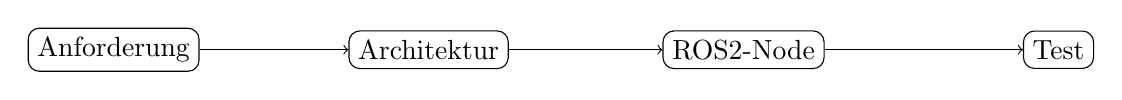
\begin{tikzpicture}[node distance=1.6cm]
\node (req) [draw, rounded corners] {Anforderung};
\node (arch) [draw, rounded corners, right of=req, xshift=2.4cm] {Architektur};
\node (impl) [draw, rounded corners, right of=arch, xshift=2.4cm] {ROS2-Node};
\node (test) [draw, rounded corners, right of=impl, xshift=2.4cm] {Test};
\draw[->] (req) -- (arch);
\draw[->] (arch) -- (impl);
\draw[->] (impl) -- (test);
\end{tikzpicture}
\end{center}

\section{Grenzen von MBSE}
MBSE löst keine schlechten technischen Entscheidungen. Ein Modell kann falsch, veraltet oder unnötig kompliziert sein. Der Nutzen entsteht nur, wenn das Modell gepflegt wird und echte Entscheidungen unterstützt.

\begin{uebungbox}
Erstellen Sie eine Tabelle mit drei Spalten: Information, klassischer Speicherort und Speicherort im MBSE-Modell. Tragen Sie Anforderungen, Schnittstellen, Tests und ROS2-Nodes ein.
\end{uebungbox}

\chapter{SysML-Grundlagen}

\begin{lernziele}
Nach diesem Kapitel kennen Sie die wichtigsten SysML-Diagrammtypen und wissen, wofür sie eingesetzt werden.
\end{lernziele}

\section{Was ist SysML?}
\gls{sysml} steht für Systems Modeling Language. Die Sprache wurde entwickelt, um technische Systeme modellieren zu können. Sie basiert auf UML, ist aber stärker auf Systeme aus Hardware, Software, Menschen, Prozessen und physikalischen Zusammenhängen ausgerichtet.

\section{Diagrammtypen}
Für den Einstieg sind sechs Diagrammtypen besonders wichtig.

\subsection{Requirement Diagram}
Das Requirement Diagram beschreibt Anforderungen und ihre Beziehungen. Es zeigt, welche Anforderungen voneinander abhängen und welche Elemente sie erfüllen oder verifizieren.

\subsection{Block Definition Diagram}
Das \gls{bdd} beschreibt die Systemstruktur auf einer eher abstrakten Ebene. Es zeigt Blöcke und ihre Beziehungen.

\subsection{Internal Block Diagram}
Das \gls{ibd} zeigt die innere Struktur eines Blocks. Es zeigt Teile, Ports und Verbindungen.

\subsection{Activity Diagram}
Aktivitätsdiagramme beschreiben Abläufe. Sie eignen sich für Prozesse, Algorithmen und Betriebsabläufe.

\subsection{State Machine Diagram}
Zustandsdiagramme beschreiben Zustände und Übergänge. Sie sind besonders nützlich für Systeme mit klaren Betriebsmodi.

\subsection{Parametric Diagram}
Parametrische Diagramme beschreiben mathematische Beziehungen, zum Beispiel Energieverbrauch oder Reichweite.

\section{Nicht alles gleichzeitig lernen}
Einsteiger sollten nicht versuchen, sofort jedes Diagramm perfekt zu beherrschen. Der sinnvolle Einstieg lautet: Anforderungen, BDD, IBD, Aktivitätsdiagramm und Zustandsdiagramm. Parametrik kann später folgen.

\begin{praxisbox}
Für den Indoor-Roboter beginnen wir mit Anforderungen und Struktur. Erst wenn klar ist, was der Roboter können soll und aus welchen Hauptsystemen er besteht, modellieren wir Verhalten und technische Details.
\end{praxisbox}

\section{Modell statt Bild}
Ein SysML-Diagramm ist nur eine Sicht auf ein Modell. Das ist wichtig: Wenn ein Block in mehreren Diagrammen erscheint, ist es derselbe Block. Wird der Name geändert, sollte sich die Änderung überall widerspiegeln. Gute Modellierungswerkzeuge speichern also nicht nur Zeichnungen, sondern Modellinformationen.

\begin{uebungbox}
Ordnen Sie folgende Fragen einem Diagrammtyp zu: Was muss das System leisten? Aus welchen Teilen besteht es? Welche Daten fließen zwischen Komponenten? Welche Zustände kann der Roboter haben?
\end{uebungbox}

\chapter{Werkzeuge für SysML v2 einrichten}

\begin{lernziele}
Nach diesem Kapitel können Sie erklären, warum dieses Lehrbuch eine textuelle SysML-v2-Arbeitsweise verwendet. Sie können ein einfaches Projekt in VS Code mit dem Syside Editor anlegen, SysML-v2-Dateien strukturieren und grafische Sichten als Ergänzung einordnen. Außerdem verstehen Sie, warum ein Werkzeug fachliches Modellieren unterstützt, aber nicht ersetzt.
\end{lernziele}

\section{Einleitung}
SysML v2 kann grafisch und textuell verwendet werden. Für dieses Lehrbuch steht die textuelle Notation im Vordergrund. Das passt gut zu modernen Entwicklungsabläufen: Modelle liegen in Dateien, können versioniert, verglichen, überprüft und gemeinsam mit Code gepflegt werden.

Als kostenloser Einstieg eignet sich der Syside Editor für VS Code. Er unterstützt SysML-v2-Dateien mit Syntaxhervorhebung, Autovervollständigung, Formatierung, Gliederung und Validierung. Für grafische Sichten kann zusätzlich Eclipse SysON genutzt werden. SysON ist ein webbasiertes Open-Source-Werkzeug für SysML-v2-Modelle.

\begin{hinweisbox}
Ein Werkzeug löst keine Modellierungsaufgabe automatisch. Es hilft beim Schreiben, Prüfen und Anzeigen des Modells. Die fachliche Entscheidung bleibt Ihre Aufgabe: Welche Elemente gibt es? Welche Beziehungen sind wichtig? Welche Anforderungen müssen nachverfolgbar sein?
\end{hinweisbox}

\section{Warum textuelle Modellierung?}
Viele Einsteiger erwarten bei SysML zuerst Diagramme. Diagramme bleiben wichtig, aber SysML v2 macht den Modellinhalt stärker als präzisen Text zugänglich. Ein Modell kann dadurch ähnlich behandelt werden wie Quellcode.

Textuelle Modellierung hat mehrere Vorteile:

\begin{itemize}
    \item Modelle lassen sich in Git versionieren.
    \item Änderungen sind als Textvergleich sichtbar.
    \item Beispiele können direkt im Lehrbuch gezeigt werden.
    \item Modellteile können leichter wiederverwendet werden.
    \item Validierung und Automatisierung werden einfacher.
    \item ROS2-Code und SysML-v2-Modell können im selben Projekt liegen.
\end{itemize}

Das bedeutet nicht, dass Diagramme unwichtig werden. Diagramme sind weiterhin wertvolle Sichten. Der Unterschied ist: Das Modell entsteht nicht nur durch Zeichnen, sondern durch präzise definierte Modellelemente.

\section{Empfohlene Werkzeugkette}
Für dieses Lehrbuch verwenden wir eine einfache Werkzeugkette:

\begin{itemize}
    \item VS Code als Editor
    \item Syside Editor als SysML-v2-Erweiterung
    \item Git für Versionsverwaltung
    \item optional Eclipse SysON für grafische Sichten
    \item optional das SysML-v2-Pilotprojekt als Referenz für fortgeschrittene Experimente
\end{itemize}

Diese Auswahl ist bewusst pragmatisch. Sie ist kostenlos zugänglich, passt zu textueller Modellierung und überfordert Einsteiger weniger als große industrielle Modellierungsumgebungen.

\section{Projekt anlegen}
Für das Lehrbuch verwenden wir ein Projekt mit dem Namen \texttt{AutonomousIndoorRobot}. Der Name ist bewusst englisch, weil spätere ROS2-Pakete, Nodes und Topics ebenfalls englische technische Bezeichnungen verwenden. Die erklärenden Texte im Modell können trotzdem deutsch sein.

Eine einfache Projektstruktur kann so aussehen:

\begin{verbatim}
AutonomousIndoorRobot/
  model/
    00_overview.sysml
    01_context.sysml
    02_requirements.sysml
    03_structure.sysml
    04_behavior.sysml
    05_interfaces.sysml
    06_tests.sysml
    07_ros2_mapping.sysml
  code/
    status_node.py
    battery_monitor_node.py
  docs/
    decisions.md
\end{verbatim}

Die Dateien im Ordner \texttt{model} enthalten das SysML-v2-Modell. Der Ordner \texttt{code} enthält spätere ROS2-Beispiele. Der Ordner \texttt{docs} kann kurze Architekturentscheidungen aufnehmen.

\section{Erste SysML-v2-Datei}
Eine erste Datei \texttt{00\_overview.sysml} kann den Projektrahmen beschreiben:

\begin{lstlisting}
package AutonomousIndoorRobot {
  doc
  /* Ein Lernmodell für einen autonomen Indoor-Roboter.
     Das Modell verbindet Anforderungen, Struktur, Verhalten,
     Schnittstellen, ROS2-Mapping und Tests. */

  part def Robot;
}
\end{lstlisting}

Dieses Beispiel ist noch sehr klein. Es zeigt aber bereits eine wichtige Idee: Das System wird nicht als loses Bild begonnen, sondern als benannter Modellraum mit einem ersten Systemelement.

\section{Empfohlene Modellstruktur}
Die Modellstruktur orientiert sich an den wichtigsten Fragen des Projekts:

\begin{itemize}
    \item \texttt{00\_overview.sysml}: Ziel, Umfang und Systemgrenze
    \item \texttt{01\_context.sysml}: Stakeholder, externe Systeme und Umgebung
    \item \texttt{02\_requirements.sysml}: Anforderungen und Beziehungen
    \item \texttt{03\_structure.sysml}: Systemteile, Subsysteme und Komponenten
    \item \texttt{04\_behavior.sysml}: Aktionen, Abläufe und Zustände
    \item \texttt{05\_interfaces.sysml}: Ports, Verbindungen und Datenflüsse
    \item \texttt{06\_tests.sysml}: Testfälle und Verifikation
    \item \texttt{07\_ros2\_mapping.sysml}: Zuordnung zu ROS2-Nodes, Topics, Services und Actions
\end{itemize}

Diese Struktur ist bewusst schlicht. Sie trennt die wichtigsten Modellbereiche, ohne schon zu Beginn ein kompliziertes Metamodell einzuführen.

\section{Namenskonventionen}
Klare Namen machen Modelle lesbar. Für dieses Lehrbuch verwenden wir einfache Regeln:

\begin{itemize}
    \item Packages: \texttt{AutonomousIndoorRobot}
    \item Part Definitions: \texttt{Robot}, \texttt{BatterySystem}, \texttt{NavigationSystem}
    \item Parts: \texttt{batterySystem}, \texttt{navigationSystem}
    \item Actions: \texttt{MonitorBattery}, \texttt{NavigateToGoal}
    \item Requirements: \texttt{REQ\_DetectObstacles}, \texttt{REQ\_ReturnToDock}
    \item Testfälle: \texttt{TC\_BatteryLowReturn}
    \item ROS2-Nodes: \texttt{battery\_monitor\_node}
    \item Topics: \texttt{/battery\_state}, \texttt{/cmd\_vel}
\end{itemize}

Vermeiden Sie wechselnde Namen für dasselbe Element. Wenn ein Element einmal \texttt{BatterySystem} heißt, sollte es nicht an anderer Stelle \texttt{PowerModule} genannt werden, außer Sie modellieren bewusst unterschiedliche Dinge.

\section{Grafische Sichten}
Grafische Sichten sind besonders hilfreich, wenn ein Team schnell über Struktur oder Schnittstellen sprechen möchte. In SysML v2 sollte man sie als Darstellung des Modells verstehen, nicht als Ersatz für das Modell.

Eclipse SysON kann für solche Sichten interessant sein. Es ist besonders dann nützlich, wenn Sie aus dem textuellen Modell heraus Struktur-, Verbindungs- oder Anforderungssichten visualisieren wollen. Für den Einstieg in diesem Buch reicht es aber, zunächst die textuelle Notation sauber zu verstehen.

\section{Typische Anfängerfehler}
\subsection{Text wie Programmcode ohne Bedeutung schreiben}
SysML-v2-Text sieht teilweise wie Code aus. Trotzdem modellieren Sie kein Programm, sondern ein System. Fragen Sie bei jedem Element: Welche fachliche Aussage steckt dahinter?

\subsection{Zu früh zu viele Dateien anlegen}
Eine klare Struktur hilft, aber zu viele leere Dateien machen den Einstieg schwer. Beginnen Sie mit Überblick, Anforderungen und Struktur. Verhalten, Tests und Mapping können anschließend wachsen.

\subsection{Diagramme als Wahrheit behandeln}
Ein Diagramm zeigt nur eine Sicht. Die eigentliche Wahrheit liegt im Modell und seinen Beziehungen. Wenn Diagramm und Modell auseinanderlaufen, muss das Modell geklärt werden.

\subsection{Werkzeugvalidierung mit Modellqualität verwechseln}
Ein syntaktisch gültiges Modell kann fachlich trotzdem schlecht sein. Validierung findet Schreibfehler und Regelverstöße, aber keine unklare Systemgrenze oder fehlende Sicherheitsanforderung.

\section{Zusammenfassung}
Dieses Lehrbuch verwendet SysML v2 textuell und einsteigerfreundlich. VS Code mit dem Syside Editor ist die empfohlene kostenlose Arbeitsumgebung. Eclipse SysON kann grafische Sichten ergänzen. Entscheidend bleibt aber nicht das Werkzeug, sondern ein verständliches, konsistentes und nachverfolgbares Modell.

\section{Kontrollfragen}
\begin{enumerate}
    \item Warum eignet sich textuelle Modellierung gut für SysML v2?
    \item Welche Rolle spielt der Syside Editor in diesem Lehrbuch?
    \item Warum sind grafische Sichten trotzdem nützlich?
    \item Welche Dateien enthält die empfohlene Modellstruktur?
    \item Warum sollten Modellelemente einheitlich benannt werden?
    \item Warum ersetzt Werkzeugvalidierung keine fachliche Modellprüfung?
\end{enumerate}

\section{Übungen}
\begin{uebungbox}
\textbf{Übung 1: Projektstruktur anlegen}\\
Legen Sie die empfohlene Ordnerstruktur für \texttt{AutonomousIndoorRobot} an. Erstellen Sie eine Datei \texttt{00\_overview.sysml} und beschreiben Sie Ziel, Umfang und Systemgrenze des Roboterprojekts.
\end{uebungbox}

\begin{uebungbox}
\textbf{Übung 2: Namensregeln anwenden}\\
Formulieren Sie Namen für fünf Anforderungen, drei Testfälle, fünf Part Definitions und vier ROS2-Topics. Achten Sie auf einheitliche Schreibweise.
\end{uebungbox}

\begin{uebungbox}
\textbf{Übung 3: Sicht statt Wahrheit}\\
Beschreiben Sie in drei Sätzen, warum ein Diagramm in SysML v2 nur eine Sicht auf das Modell ist.
\end{uebungbox}

\section{Literaturhinweise}
Für die praktische Arbeit mit SysML v2 sind die Dokumentation des Syside Editors, das Eclipse-SysON-Projekt und das SysML-v2-Pilotprojekt hilfreich \cite{syside,syson,sysmlv2pilot}. Für die fachliche Einordnung bleiben klassische SysML- und MBSE-Grundlagen nützlich, müssen aber bewusst auf SysML v2 übertragen werden.

\chapter{Das Praxisprojekt: Autonomer Indoor-Roboter}

\begin{lernziele}
Nach diesem Kapitel kennen Sie das Beispielsystem, seine Hauptfunktionen und die wichtigsten Randbedingungen.
\end{lernziele}

\section{Ziel des Systems}
Der autonome Indoor-Roboter soll sich in Innenräumen bewegen, Hindernisse erkennen, Personen erkennen, Ziele anfahren und bei niedrigem Akkustand zur Ladestation zurückkehren.

\section{Warum dieses Beispiel?}
Das Beispiel verbindet mehrere typische Bereiche moderner Systementwicklung: Sensorik, Aktorik, Software, Datenverarbeitung, Robotik, künstliche Intelligenz und Tests. Es ist komplex genug, damit SysML Sinn ergibt, aber nicht so groß, dass Einsteiger den Überblick verlieren.

\section{Hauptfunktionen}
\begin{itemize}
\item Umgebung erfassen
\item Karte erstellen oder laden
\item Position bestimmen
\item Navigationsziel empfangen
\item Pfad planen
\item Hindernissen ausweichen
\item Personen erkennen
\item Batterie überwachen
\item Ladestation anfahren
\end{itemize}

\section{Systemkontext}
Der Roboter interagiert mit Nutzern, Räumen, Hindernissen, Ladestation und Wartungspersonal. Diese externen Elemente gehören nicht alle zwingend zum System, beeinflussen aber Anforderungen und Schnittstellen.

\section{Annahmen}
Für dieses Lehrbuch nehmen wir an, dass der Roboter mit Kamera, Lidar, mobilem Rechner, Motorcontroller und Batterie ausgestattet ist. Als Softwarebasis verwenden wir ROS2. Für die Personenerkennung wird später ein ML-Modell eingebunden.

\begin{hinweisbox}
Das Projekt ist didaktisch vereinfacht. Ein echter sicherheitskritischer Roboter würde zusätzliche Sicherheitsanalysen, Normenbetrachtungen und Zulassungsprozesse benötigen.
\end{hinweisbox}

\begin{uebungbox}
Zeichnen Sie eine einfache Kontextskizze: Roboter in der Mitte, außen Nutzer, Hindernis, Ladestation, Raum und Wartungstechniker.
\end{uebungbox}

\chapter{Anforderungen modellieren}

\begin{lernziele}
Nach diesem Kapitel können Sie Anforderungen verständlich, eindeutig und prüfbar formulieren. Sie können Anforderungen nummerieren, strukturieren, in funktionale und nicht-funktionale Anforderungen unterscheiden und mit SysML-Beziehungen verbinden. Außerdem verstehen Sie, wie Anforderungen im Roboterprojekt von Stakeholderbedürfnissen bis zu Testfällen nachverfolgt werden.
\end{lernziele}

\section{Einleitung}
Anforderungen sind eine der wichtigsten Grundlagen eines Systemmodells. Sie beschreiben, was das System leisten muss und unter welchen Bedingungen es dies tun soll. Ohne gute Anforderungen ist unklar, welche Architektur sinnvoll ist und woran der Projekterfolg gemessen wird.

Beim autonomen Indoor-Roboter klingen viele Wünsche zunächst einfach: Der Roboter soll sicher fahren, Hindernisse erkennen, Personen erkennen, lange genug fahren und leicht bedienbar sein. Für die Entwicklung reicht das nicht. Solche Wünsche müssen in Anforderungen übersetzt werden, die eindeutig und später überprüfbar sind.

\section{Was ist eine gute Anforderung?}
Eine gute Anforderung ist:

\begin{itemize}
    \item verständlich
    \item eindeutig
    \item notwendig
    \item realistisch
    \item prüfbar
    \item möglichst lösungsneutral
\end{itemize}

\enquote{Der Roboter soll gut navigieren} ist keine gute Anforderung. Was bedeutet \enquote{gut}? Schnell? Genau? Sicher? Ohne Kollision? In unbekannten Räumen? Eine bessere Formulierung lautet:

\begin{quote}
Der Roboter muss in einem bekannten Innenraum ein ausgewähltes Ziel autonom anfahren und dabei statische Hindernisse im Fahrweg vermeiden.
\end{quote}

Auch diese Anforderung kann später noch präziser werden, aber sie ist deutlich verständlicher.

\section{Vom Bedürfnis zur Anforderung}
Stakeholder äußern häufig Bedürfnisse. Diese Bedürfnisse sind wichtig, aber noch keine technischen Anforderungen.

\begin{center}
\begin{tabular}{p{0.38\textwidth}p{0.50\textwidth}}
\toprule
\textbf{Bedürfnis} & \textbf{Mögliche Anforderung} \\
\midrule
Der Roboter soll niemanden gefährden. & Der Roboter muss bei einem Hindernis im Abstand von 0,5 m seine Geschwindigkeit reduzieren und bei 0,2 m stoppen. \\
Der Roboter soll einfach bedienbar sein. & Ein Transportauftrag muss mit höchstens drei Eingaben gestartet werden können. \\
Der Roboter soll nicht liegen bleiben. & Der Roboter muss bei niedrigem Akkustand automatisch zur Ladestation zurückkehren. \\
Wartung soll einfach sein. & Der Roboter muss Sensorstatus, Akkustatus und Fehlermeldungen anzeigen. \\
\bottomrule
\end{tabular}
\end{center}

\section{Beispielanforderungen}
\begin{longtable}{p{0.16\textwidth}p{0.69\textwidth}}
\toprule
ID & Anforderung\\
\midrule
REQ-001 & Der Roboter muss autonom in einem bekannten Innenraumbereich navigieren können.\\
REQ-002 & Der Roboter muss Hindernisse im Fahrbereich erkennen.\\
REQ-003 & Der Roboter muss erkannte Hindernisse umfahren oder rechtzeitig stoppen.\\
REQ-004 & Der Roboter muss Personen im Kamerabild erkennen können.\\
REQ-005 & Der Roboter muss seinen Akkustand überwachen.\\
REQ-006 & Der Roboter muss bei niedrigem Akkustand selbstständig zur Ladestation fahren.\\
REQ-007 & Der Roboter muss seinen Betriebszustand melden.\\
REQ-008 & Der Roboter muss einen sicheren Zustand einnehmen, wenn ein kritischer Sensor ausfällt.\\
REQ-009 & Der Roboter muss Transportaufträge über eine einfache Benutzerschnittstelle entgegennehmen.\\
REQ-010 & Der Roboter muss relevante Fehler für Wartungspersonal nachvollziehbar protokollieren.\\
\bottomrule
\end{longtable}

\section{Funktionale und nicht-funktionale Anforderungen}
Funktionale Anforderungen beschreiben, was das System tun soll. Beispiele sind Navigation, Hinderniserkennung, Akkustandsüberwachung oder Statusmeldung.

Nicht-funktionale Anforderungen beschreiben Eigenschaften des Systems. Beispiele sind Geschwindigkeit, Genauigkeit, Verfügbarkeit, Sicherheit, Wartbarkeit, Datenschutz oder Energieverbrauch.

Beide Arten sind wichtig. Ein Roboter, der alle Funktionen besitzt, aber zu langsam, unsicher oder unwartbar ist, erfüllt das Projektziel nicht.

\section{Anforderungen strukturieren}
In größeren Projekten werden Anforderungen hierarchisch strukturiert. Eine oberste Anforderung kann in mehrere konkrete Anforderungen zerlegt werden.

Beispiel:

\begin{itemize}
    \item REQ-SAFE-001: Der Roboter muss sicher in der Nähe von Menschen betrieben werden.
    \item REQ-SAFE-002: Der Roboter muss Hindernisse im Fahrweg erkennen.
    \item REQ-SAFE-003: Der Roboter muss bei Gefahr stoppen.
    \item REQ-SAFE-004: Der Roboter muss bei Sensorausfall einen sicheren Zustand einnehmen.
\end{itemize}

Die allgemeine Sicherheitsanforderung wird dadurch handhabbarer.

\section{SysML-Beziehungen}
Wichtige Beziehungen in SysML sind:

\begin{itemize}
    \item \texttt{derive}: Eine Anforderung wird aus einer anderen abgeleitet.
    \item \texttt{satisfy}: Ein Modellelement erfüllt eine Anforderung.
    \item \texttt{verify}: Ein Testfall überprüft eine Anforderung.
    \item \texttt{trace}: Eine allgemeine Nachverfolgungsbeziehung.
    \item \texttt{refine}: Ein Element beschreibt eine Anforderung genauer.
\end{itemize}

\begin{praxisbox}
REQ-002 \enquote{Hindernisse erkennen} wird durch das \texttt{PerceptionSystem} erfüllt. Der Testfall \texttt{TC-002 Hinderniserkennung} verifiziert diese Anforderung. Eine \texttt{trace}-Beziehung kann zusätzlich zeigen, dass der ROS2-Node \texttt{obstacle\_detector\_node} zur Umsetzung gehört.
\end{praxisbox}

Abbildung~\ref{fig:kap06-traceability-req002} stellt diese Traceability-Kette grafisch dar: \texttt{satisfy} und \texttt{verify} zeigen als zwei getrennte, eingehende Beziehungen auf das \texttt{PerceptionSystem}, von dort führt \texttt{trace} weiter zum ROS2-Node.

\begin{figure}[H]
  \centering
  \adjustbox{max width=\linewidth,max totalheight=0.6\textheight}{% =====================================================================
% Abbildung: Traceability-Kette am Beispiel REQ-002
% Passend zu Kapitel 6, Abschnitt "SysML-Beziehungen"
%
% Einbindung im Buch, z. B. in chapters/06_anforderungen.tex:
%
%   \begin{figure}[H]
%     \centering
%     \input{figures/fig_kap06_traceability_req002}
%     \caption{Traceability-Kette von REQ-002 ueber \texttt{satisfy} und
%       \texttt{verify} zum \texttt{PerceptionSystem} und per \texttt{trace}
%       weiter zum ROS2-Node.}
%     \label{fig:kap06-traceability-req002}
%   \end{figure}
%
% Benoetigte Pakete (im Buch bereits in main.tex geladen): tikz
% Benoetigte TikZ-Bibliotheken: positioning, arrows.meta, shadows, calc
% =====================================================================

\input{figures/fig_kap06_traceability_req002.tikz}
}
  \caption{Traceability-Kette von REQ-002 über \texttt{satisfy} und \texttt{verify} zum \texttt{PerceptionSystem} und per \texttt{trace} weiter zum ROS2-Node.}
  \label{fig:kap06-traceability-req002}
\end{figure}

\section{Anforderungen in SysML v2}
In SysML v2 werden Anforderungen – eingebettet in ein \texttt{package} wie bereits aus Kapitel 3 bekannt – textuell mit dem Schlüsselwort \texttt{requirement} definiert:

\begin{lstlisting}
package Requirements {

  requirement REQ_001 {
    doc /* Der Roboter muss in einem bekannten Innenraumbereich
           autonom navigieren koennen. */
  }

  requirement REQ_SAFE {
    doc /* Sicherheitsanforderungen. */
    requirement REQ_SAFE_001 {
      doc /* Der Roboter muss Hindernisse im Fahrweg erkennen. */
      derive REQ_001;
    }
  }
}
\end{lstlisting}

Anders als bei \texttt{part def} und \texttt{part} in Kapitel 8 unterscheidet SysML v2 bei \texttt{requirement} im Grundfall nicht zwischen Typ und Nutzung: Das Schlüsselwort \texttt{requirement} definiert die Anforderung im Beispiel gleichzeitig als solche.

Erstellen Sie in der Datei \texttt{02\_requirements.sysml} erste Requirement-Elemente. Verwenden Sie klare Namen, eine stabile ID und einen prüfbaren Text. Achten Sie darauf, dass Anforderungen nicht nur als Liste existieren, sondern später mit Systemteilen, Verhalten und Tests verbunden werden.

Nutzen Sie Beschreibungsfelder (\texttt{doc /* ... */}), um Annahmen, Begründungen oder offene Fragen zu dokumentieren. Wenn eine Anforderung noch unklar ist, markieren Sie sie bewusst, statt sie stillschweigend als fertig zu behandeln – zum Beispiel mit einem kurzen \texttt{doc /* TBD: ... */}-Vermerk im betroffenen Requirement-Element.

\section{Typische Fehler}
\subsection{Zu allgemeine Anforderungen}
\enquote{Der Roboter soll zuverlässig sein} ist nicht prüfbar. Besser sind konkrete Kriterien.

\subsection{Lösungen als Anforderungen}
\enquote{Der Roboter muss Sensor X verwenden} ist häufig bereits eine Designentscheidung. Besser ist eine lösungsneutrale Fähigkeit, sofern kein konkreter Sensor vorgeschrieben ist.

\subsection{Keine Akzeptanzkriterien}
Eine Anforderung sollte erkennen lassen, wie sie später geprüft wird. Ein Akzeptanzkriterium legt fest, woran sich die Erfüllung konkret zeigt, zum Beispiel: \enquote{Testfall: Bei einem simulierten Hindernis in 0,5\,m Abstand muss die Geschwindigkeit innerhalb 1\,s reduziert werden.} Ohne solche Kriterien entstehen Diskussionen am Projektende.

\subsection{Keine Pflege}
Anforderungen ändern sich. Wichtig ist, Änderungen nachvollziehbar zu halten und betroffene Modellelemente zu prüfen.

\section{Vertiefungsbeispiel: Batteriemanagement mit abgesicherter Rückkehr}
\label{sec:bm-anforderungen}
Die Anforderungen REQ-005 und REQ-006 beschreiben zunächst Akkustandsüberwachung und Rückkehr bei niedrigem Akkustand. Wir verfeinern diese Ausgangslage: Der Roboter soll anhand des bisherigen Verbrauchs abschätzen, ob er den laufenden Transportauftrag noch abschließen und anschließend zur Ladestation zurückkehren kann. Ein fester Akkuschwellwert allein beantwortet diese Frage nicht.

Dieses Beispiel ist ein fachlicher Entwurf. Die folgenden BM-Anforderungen ergänzen die bisherigen Lehrbuchbeispiele; ihre Umsetzung in SysML und ROS2 sowie der Nachweis am Roboter stehen noch aus. Der Entscheidungsablauf folgt in Abschnitt~\ref{sec:bm-ablauf}, die Energiebilanz in Abschnitt~\ref{sec:bm-energie} und die Testzuordnung in Abschnitt~\ref{sec:bm-tests}.

\subsection{Systemgrenze und Annahmen}
Betrachtet werden Akkuzustand, Verbrauchserfassung, Energiebedarfsschätzung, Rückwegabsicherung, Auftragsentscheidung, Navigation und Statusmeldungen. Die Ladestation ist ein externes System. Die Rückkehr endet erst mit bestätigtem Andocken und Ladebeginn.

Als Entwurfsannahme beginnt die Fahrt an einer bekannten Ladestation. Der Roboter zeichnet den gefahrenen Weg und dessen Energieverbrauch auf und kann dem Weg zurück folgen. Diese vorgeschlagenen Fähigkeiten müssen technisch geprüft werden. Ein bereits gefahrener Weg ist weder automatisch in Gegenrichtung befahrbar noch dauerhaft frei. Auch der Rückwegverbrauch darf nicht ungeprüft mit dem Hinwegverbrauch gleichgesetzt werden.

Ein \emph{abgesicherter Rückweg} besitzt einen bekannten Verlauf, ist ausreichend zuverlässig verfolgbar und wurde hinsichtlich Befahrbarkeit und Energiebedarf einschließlich Andocken bewertet. Eine \emph{belastbare Schätzung} verwendet gültige Eingangsdaten und berücksichtigt ihre Unsicherheit. Welche Qualität hierfür genügt, bleibt ein offener Projektparameter.

\begin{hinweisbox}
Sind Restauftrag oder vorgesehener Rückweg nicht abschätzbar, etwa wegen fehlender Kartendaten, darf der Auftrag nicht fortgesetzt werden. Die Rückkehr muss dann durch eine unabhängig abgesicherte Möglichkeit gewährleistet werden, beispielsweise durch eine geeignete Wegaufzeichnung. Eine fehlende Schätzung ist kein geringer Energiebedarf.
\end{hinweisbox}

\subsection{Anforderungen des Vertiefungsbeispiels}
Die IDs BM-01 bis BM-13 bleiben über Anforderungen, Ablauf und Tests hinweg stabil. BM-06 legt bewusst eine Entwurfsentscheidung für dieses Beispiel fest; eine andere technische Rückkehrstrategie wäre gesondert zu bewerten.

\begin{description}[style=nextline]
    \item[BM-01: Startfreigabe] Vor Fahrtbeginn muss der Roboter gültige Akkudaten, Verbrauchserfassung und eine verfügbare Rückkehrstrategie prüfen. Fehlt eine Voraussetzung, darf kein Transportauftrag starten.
    \item[BM-02: Verbrauchsbasierte Schätzung] Der Roboter muss den bisherigen Energieverbrauch erfassen und damit den geschätzten Bedarf aktualisieren. Veränderungen von Last, Fahrprofil oder Umgebung müssen in die Bewertung eingehen.
    \item[BM-03: Entscheidungsgrundlage] Für jede Auftragsentscheidung muss der Roboter nutzbare Restenergie, Bedarf des Restauftrags, anschließenden Rückkehrbedarf und Reserve mit Gültigkeit und Unsicherheit bewerten. Unbekannte Werte dürfen nicht als null gelten.
    \item[BM-04: Auftrag fortsetzen] Der Roboter darf den Auftrag nur fortsetzen, wenn Restauftrag, anschließende Rückkehr und Reserve durch eine belastbare Energieschätzung gedeckt sind. Zusätzlich muss eine Rückkehr vom aktuellen Standort abgesichert bleiben.
    \item[BM-05: Fehlende Abschätzbarkeit] Sind Restauftrag oder anschließender Rückweg nicht abschätzbar, muss der Roboter den Auftrag kontrolliert unterbrechen und eine abgesicherte Rückkehr beginnen. Ein hoher Akkustand hebt diese Regel nicht auf.
    \item[BM-06: Wegaufzeichnung] Der Roboter muss den gefahrenen Weg und zugehörige Verbrauchsdaten für die Rückkehrbewertung aufzeichnen. Lücken und ungültige Abschnitte müssen erkannt und berücksichtigt werden.
    \item[BM-07: Rückwegfreigabe] Ein aufgezeichneter Weg darf nur bei bewerteter Verfolgbarkeit, Befahrbarkeit und ausreichender Energie einschließlich Reserve als abgesicherter Rückweg verwendet werden. Die Aufzeichnung allein genügt nicht.
    \item[BM-08: Laufende Absicherung] Der Roboter muss die Rückkehrabsicherung regelmäßig und bei relevanten Änderungen erneut bewerten. Droht sie verloren zu gehen, muss er die Rückkehr vor Unterschreiten der festgelegten Rückkehrgrenze einleiten. Reaktions- und Unterbrechungszeit sind zu berücksichtigen.
    \item[BM-09: Blockierter Rückweg] Bei einer Blockade muss der Roboter einen alternativen Rückweg bewerten. Er darf ihn nur bei abgesicherter Befahrbarkeit und ausreichender Energie nutzen. Auch Warte- und Planungsenergie müssen berücksichtigt werden.
    \item[BM-10: Keine abgesicherte Rückkehr] Ist kein abgesicherter Rückweg verfügbar, muss der Roboter kontrolliert anhalten und Unterstützung anfordern. Der Auftrag bleibt unterbrochen; die autonome Rückkehr muss als nicht erfüllt gemeldet werden.
    \item[BM-11: Datenausfall] Bei Ausfall von Akkudaten oder Wegaufzeichnung muss der Roboter die verbleibende Rückkehrabsicherung neu bewerten. Nur eine weiterhin belastbar abgesicherte Rückkehr darf fortgesetzt werden; andernfalls gilt BM-10.
    \item[BM-12: Nachvollziehbarer Status] Der Roboter muss Entscheidung, Entscheidungsgrund, Auftragsstatus und Rückkehrstatus nachvollziehbar melden. Fortsetzung, Unterbrechung, Rückkehr und Unterstützungsbedarf müssen unterscheidbar sein.
    \item[BM-13: Rückkehr erfolgreich] Der Roboter darf die Rückkehr erst nach bestätigtem Andocken und Ladebeginn als erfolgreich melden. Das Erreichen der Stationsposition allein genügt nicht.
\end{description}

\subsection{Offene Parameter und Nachweisgrenzen}
Vor einer Implementierung müssen das Verfahren zur Restenergieschätzung, Energiereserve, zulässige Schätzunsicherheit, Rückkehrgrenze, Prüfabstände und Kriterien für gültige Wegdaten festgelegt werden. Ebenso ist zu klären, wie ein kontrolliertes Anhalten bei der vorgesehenen Ladung und Umgebung aussieht. Konkrete Werte werden hier bewusst nicht erfunden.

Damit liegt noch keine technische Rückkehrgarantie vor. Insbesondere die Rückkehr ohne Karte, die Verbrauchsschätzung und unerwartete Wegblockaden benötigen einen Nachweis. Kontrolliertes Anhalten mit Unterstützungsanforderung begrenzt die Folgen eines Fehlers, erfüllt aber nicht die geforderte autonome Rückkehr.

\section{Zusammenfassung}
Anforderungen verbinden Stakeholderbedürfnisse mit Architektur und Tests. Gute Anforderungen sind verständlich, eindeutig und prüfbar. In SysML v2 werden Anforderungen nicht nur gesammelt, sondern über Beziehungen mit Systemteilen, Aktionen, Schnittstellen und Testfällen verbunden.

\section{Kontrollfragen}
\begin{enumerate}
    \item Was macht eine gute Anforderung aus?
    \item Warum ist \enquote{Der Roboter soll gut navigieren} problematisch?
    \item Was ist der Unterschied zwischen funktionalen und nicht-funktionalen Anforderungen?
    \item Wozu dient \texttt{derive}?
    \item Wozu dient \texttt{satisfy}?
    \item Wozu dient \texttt{verify}?
    \item Warum sollten Anforderungen möglichst lösungsneutral sein?
    \item Welche Anforderung könnte aus dem Bedürfnis \enquote{Wartung soll einfach sein} entstehen?
\end{enumerate}

\section{Übungen}
\begin{uebungbox}
\textbf{Übung 1: Anforderungen formulieren}\\
Formulieren Sie fünf zusätzliche Anforderungen: zwei zur Sicherheit, eine zur Bedienung, eine zur Wartung und eine zur Leistung.
\end{uebungbox}

\begin{uebungbox}
\textbf{Übung 2: Anforderungen verbessern}\\
Verbessern Sie die Aussagen \enquote{Der Roboter soll schnell sein}, \enquote{Der Roboter soll zuverlässig sein} und \enquote{Die Bedienung soll intuitiv sein}, sodass daraus prüfbare Anforderungen werden.
\end{uebungbox}

\begin{uebungbox}
\textbf{Übung 3: Beziehungen anlegen}\\
Wählen Sie drei Anforderungen aus der Tabelle. Ordnen Sie jeder Anforderung ein Systemelement (\texttt{part def}) und einen Testfall zu.
\end{uebungbox}

\section{Literaturhinweise}
Anforderungsmodellierung ist ein zentraler Bestandteil von SysML und MBSE. Für den Einstieg eignen sich Delligatti \cite{delligatti2014} sowie Friedenthal, Moore und Steiner \cite{friedenthal2014}. Für reale Projekte sollte zusätzlich Literatur zum Requirements Engineering genutzt werden.

\chapter{Stakeholder und Use Cases}

\begin{lernziele}
Nach diesem Kapitel können Sie Stakeholder identifizieren und aus typischen Nutzungsszenarien Anforderungen ableiten.
\end{lernziele}

\section{Stakeholder identifizieren}
Stakeholder sind nicht nur Endnutzer. Auch Betreiber, Wartung, Entwicklung, Management und Sicherheitsverantwortliche haben Interessen. Ein Roboter, der technisch funktioniert, aber schlecht wartbar ist, kann im Betrieb trotzdem scheitern.

\section{Stakeholder des Roboters}
\begin{itemize}
\item Nutzer: möchte Ziele einfach vorgeben.
\item Betreiber: möchte zuverlässigen Betrieb.
\item Wartungstechniker: benötigt Diagnoseinformationen.
\item Entwickler: benötigt klare Schnittstellen.
\item Sicherheitsverantwortlicher: achtet auf Risiken.
\end{itemize}

\section{Use Cases}
Use Cases beschreiben, wie ein Akteur mit dem System interagiert. Sie sind keine detaillierten Algorithmen, sondern Nutzungsbeschreibungen.

\section{Beispiel: Ziel anfahren}
\textbf{Akteur:} Nutzer\\
\textbf{Ziel:} Roboter fährt zu einem ausgewählten Zielpunkt.\\
\textbf{Vorbedingung:} Roboter ist eingeschaltet und lokalisiert.\\
\textbf{Ablauf:}
\begin{enumerate}
\item Nutzer wählt Ziel.
\item Roboter prüft Verfügbarkeit der Karte.
\item Roboter plant Pfad.
\item Roboter fährt los.
\item Roboter weicht Hindernissen aus.
\item Roboter erreicht Ziel.
\end{enumerate}

\section{Use Cases und Anforderungen}
Aus einem Use Case lassen sich Anforderungen ableiten. Wenn der Roboter Ziele anfahren soll, braucht er Navigation, Lokalisierung, Pfadplanung und Hindernisvermeidung.

\begin{uebungbox}
Schreiben Sie einen Use Case \enquote{Zur Ladestation zurückkehren}. Leiten Sie daraus mindestens drei Anforderungen ab.
\end{uebungbox}

\chapter{Block Definition Diagram}

\begin{lernziele}
Nach diesem Kapitel können Sie die Hauptstruktur des Roboters als Block Definition Diagram modellieren.
\end{lernziele}

\section{Zweck des BDD}
Das \gls{bdd} zeigt, aus welchen logischen oder physischen Bausteinen ein System besteht. Ein Block kann Hardware, Software, Mensch, Datenobjekt oder abstrakte Funktion darstellen.

\section{Hauptstruktur des Roboters}
\begin{verbatim}
Robot
|- NavigationSystem
|- PerceptionSystem
|- MotionControl
|- BatterySystem
|- CommunicationSystem
|- UserInterface
\end{verbatim}

Diese Darstellung ist noch grob. Sie eignet sich aber hervorragend, um den Systemumfang zu verstehen.

\section{Komposition}
Eine Komposition beschreibt eine starke Teil-Ganzes-Beziehung. Wenn das \texttt{PerceptionSystem} Teil des Roboters ist, kann dies als Komposition modelliert werden.

\section{Dekomposition}
Das \texttt{PerceptionSystem} kann weiter zerlegt werden:
\begin{verbatim}
PerceptionSystem
|- Camera
|- Lidar
|- ObjectDetector
|- ObstacleDetector
\end{verbatim}

\section{Logische und physische Blöcke}
Ein häufiger Anfängerfehler besteht darin, logische Funktionen und physische Bauteile unklar zu vermischen. \texttt{Camera} ist eher physisch. \texttt{ObjectDetector} ist eher logisch oder softwarebezogen. Beides darf im Modell vorkommen, sollte aber bewusst getrennt werden.

\begin{hinweisbox}
Ein BDD muss nicht sofort perfekt sein. Es entwickelt sich mit dem Verständnis des Systems.
\end{hinweisbox}

\begin{uebungbox}
Erstellen Sie ein BDD mit dem Block \texttt{Robot} und mindestens fünf Subsystemen. Ergänzen Sie beim \texttt{PerceptionSystem} Kamera, Lidar und Objekterkennung.
\end{uebungbox}

\chapter{Internal Block Diagram}

\begin{lernziele}
Nach diesem Kapitel können Sie Datenflüsse und interne Verbindungen zwischen Komponenten im IBD darstellen.
\end{lernziele}

\section{Zweck des IBD}
Das \gls{ibd} zeigt, wie Teile eines Blocks intern verbunden sind. Während das BDD sagt, welche Bausteine existieren, zeigt das IBD, wie sie zusammenarbeiten.

\section{Beispiel Datenfluss}
\begin{verbatim}
Camera -> ObjectDetector -> NavigationSystem
Lidar  -> SLAM           -> NavigationSystem
NavigationSystem -> MotionControl -> Motors
BatterySystem -> NavigationSystem
\end{verbatim}

\section{Ports}
Ports beschreiben Ein- und Ausgänge von Blöcken. Ein Kamerablock kann einen Port \texttt{imageOut} haben. Der ObjectDetector kann einen Port \texttt{imageIn} und \texttt{objectsOut} haben.

\section{Schnittstellen}
Eine Verbindung ohne klare Schnittstelle ist wenig wert. Deshalb sollte dokumentiert werden, welche Daten übertragen werden. Beispiel: \texttt{sensor\_msgs/Image} für Kamerabilder in ROS2.

\section{IBD und ROS2}
Das IBD passt gut zur ROS2-Kommunikation. ROS2-Topics können als Datenflüsse modelliert werden. Ein Topic \texttt{/camera/image\_raw} verbindet \texttt{camera\_node} und \texttt{object\_detector\_node}.

\begin{uebungbox}
Erstellen Sie ein IBD für das \texttt{PerceptionSystem}. Modellieren Sie Kamera, Lidar, ObjectDetector und ObstacleDetector inklusive Datenflüssen.
\end{uebungbox}

\chapter{Schnittstellenmodellierung}

\begin{lernziele}
Nach diesem Kapitel können Sie Schnittstellen beschreiben und erkennen, warum klare Schnittstellen in Robotikprojekten entscheidend sind.
\end{lernziele}

\section{Warum Schnittstellen wichtig sind}
Viele technische Probleme entstehen nicht in einzelnen Komponenten, sondern an ihren Schnittstellen. Eine Kamera liefert Bilder in einem Format, das der Erkennungsalgorithmus nicht erwartet. Ein Navigationsknoten erwartet Koordinaten in einem anderen Bezugssystem. Solche Fehler sind typisch.

\section{Schnittstellenbeschreibung}
Eine gute Schnittstellenbeschreibung enthält:
\begin{itemize}
\item Name der Schnittstelle
\item Sender und Empfänger
\item Datentyp
\item Frequenz oder Ereignis
\item Qualitätsanforderungen
\item Fehlerfälle
\end{itemize}

\section{Beispiel}
\begin{longtable}{p{35mm}p{35mm}p{35mm}p{35mm}}
\toprule
Schnittstelle & Sender & Empfänger & Datentyp\\
\midrule
Kamerabild & Camera & ObjectDetector & sensor\_msgs/Image\\
Laserscan & Lidar & SLAM & sensor\_msgs/LaserScan\\
Bewegungsbefehl & Navigation & MotionControl & geometry\_msgs/Twist\\
Akkustatus & BatterySystem & Navigation & sensor\_msgs/BatteryState\\
\bottomrule
\end{longtable}

\section{Koordinatensysteme}
In Robotikprojekten sind Koordinatensysteme kritisch. ROS2 nutzt häufig Frames wie \texttt{map}, \texttt{odom}, \texttt{base\_link} und \texttt{camera\_link}. Diese sollten im Modell dokumentiert werden.

\begin{uebungbox}
Erstellen Sie eine Schnittstellentabelle für mindestens sechs Datenflüsse des Roboters. Ergänzen Sie jeweils Sender, Empfänger und Datentyp.
\end{uebungbox}

\chapter{Verhaltensmodellierung mit Activity Diagrams}

\begin{lernziele}
Nach diesem Kapitel können Sie Abläufe des Roboters als Aktivitätsdiagramm beschreiben.
\end{lernziele}

\section{Was beschreibt ein Aktivitätsdiagramm?}
Ein Aktivitätsdiagramm beschreibt einen Ablauf aus Aktionen, Entscheidungen und Verzweigungen. Es eignet sich gut für Prozesse wie \enquote{Navigationsziel anfahren}.

\section{Beispielablauf Navigation}
\begin{enumerate}
\item System starten
\item Sensoren initialisieren
\item Karte laden
\item Ziel empfangen
\item Pfad planen
\item Bewegung ausführen
\item Hindernisse prüfen
\item Ziel erreicht melden
\end{enumerate}

\section{Entscheidungen}
Entscheidungsknoten modellieren Alternativen. Beispiel: Wenn ein Hindernis erkannt wird, plant der Roboter neu oder stoppt.

\section{Parallelität}
Ein Roboter führt oft mehrere Aktivitäten parallel aus. Während er fährt, überwacht er Sensoren und Batterie. Aktivitätsdiagramme können solche parallelen Abläufe darstellen, sollten am Anfang aber nicht überladen werden.

\begin{praxisbox}
Der Ablauf \enquote{Zur Ladestation fahren} enthält eine Entscheidung: Ist der Akkustand niedrig? Nur dann wird der Ladevorgang gestartet.
\end{praxisbox}

\begin{uebungbox}
Modellieren Sie den Ablauf \enquote{Ziel anfahren}. Ergänzen Sie mindestens eine Entscheidung für Hinderniserkennung und eine für niedrigen Akkustand.
\end{uebungbox}

\chapter{Zustandsmodellierung mit State Machines}

\begin{lernziele}
Nach diesem Kapitel können Sie Betriebszustände und Zustandswechsel eines Roboters modellieren.
\end{lernziele}

\section{Zustände}
Ein Zustand beschreibt eine Situation, in der sich das System über eine gewisse Zeit befindet. Beispiele für den Roboter sind \texttt{Idle}, \texttt{Mapping}, \texttt{Navigation}, \texttt{Charging} und \texttt{Error}.

\section{Ereignisse}
Ereignisse lösen Übergänge aus. Beispiele:
\begin{itemize}
\item \texttt{GoalReceived}
\item \texttt{BatteryLow}
\item \texttt{ObstacleDetected}
\item \texttt{ChargingComplete}
\item \texttt{ErrorDetected}
\end{itemize}

\section{Beispiel}
\begin{verbatim}
Idle --GoalReceived--> Navigation
Navigation --BatteryLow--> ReturnToDock
ReturnToDock --DockReached--> Charging
Charging --ChargingComplete--> Idle
Navigation --ErrorDetected--> Error
\end{verbatim}

\section{Warum State Machines nützlich sind}
Zustandsdiagramme verhindern unklare Logik. Sie zeigen, welche Übergänge erlaubt sind. Darf der Roboter während eines Fehlers ein neues Ziel annehmen? Darf er während des Ladens navigieren? Solche Fragen werden sichtbar.

\begin{uebungbox}
Erstellen Sie eine State Machine für den Roboter mit mindestens fünf Zuständen und acht Übergängen.
\end{uebungbox}

\chapter{Parametrische Modellierung}

\begin{lernziele}
Nach diesem Kapitel verstehen Sie, wie technische Zusammenhänge im Modell beschrieben werden können.
\end{lernziele}

\section{Zweck parametrischer Modelle}
Parametrische Modelle beschreiben mathematische Beziehungen. Sie helfen, technische Entscheidungen zu prüfen. Beim Roboter sind Energieverbrauch, Reichweite und Geschwindigkeit wichtige Größen.

\section{Einfaches Beispiel}
\[
t_{betrieb} = \frac{E_{akku}}{P_{gesamt}}
\]

Dabei ist \(E_{akku}\) die nutzbare Energie der Batterie und \(P_{gesamt}\) die durchschnittliche Leistungsaufnahme.

\section{Leistungsaufnahme}
Die Gesamtleistung kann grob abgeschätzt werden:
\[
P_{gesamt} = P_{rechner} + P_{sensoren} + P_{motoren}
\]

Diese Formel ist einfach, aber nützlich für frühe Architekturentscheidungen.

\section{Parametric Diagram in SysML}
In SysML werden solche Zusammenhänge mit Constraint Blocks modelliert. Ein Constraint Block beschreibt die Formel, Parameter werden mit Systemeigenschaften verbunden.

\begin{hinweisbox}
Parametrik ist für Einsteiger optional. Sie wird wichtig, wenn quantitative Aussagen getroffen werden sollen.
\end{hinweisbox}

\begin{uebungbox}
Nehmen Sie eine Batteriekapazität von 100 Wh und eine Leistungsaufnahme von 25 W an. Berechnen Sie die theoretische Betriebszeit.
\end{uebungbox}

\chapter{ROS2-Grundlagen}

\begin{lernziele}
Nach diesem Kapitel kennen Sie Nodes, Topics, Services und Actions und können diese Begriffe auf das Robotersystem anwenden.
\end{lernziele}

\section{Was ist ROS2?}
\gls{ros2} ist ein Framework für Robotiksoftware. Es stellt Kommunikationsmechanismen, Werkzeuge und Konventionen bereit. ROS2 ist kein Betriebssystem im klassischen Sinn, sondern eine Middleware und Entwicklungsumgebung.

\section{Nodes}
Ein Node ist ein ausführbares Programm mit einer klaren Aufgabe. Beispiel: Ein \texttt{camera\_node} liest Kamerabilder und veröffentlicht sie.

\section{Topics}
Topics sind Nachrichtenkanäle. Ein Node veröffentlicht Nachrichten, andere Nodes abonnieren sie. Diese Publish-Subscribe-Kommunikation passt sehr gut zu Sensordaten.

\section{Services}
Services sind Anfrage-Antwort-Kommunikation. Sie eignen sich für kurze, gezielte Abfragen, zum Beispiel \enquote{Setze Parameter}.

\section{Actions}
Actions sind für länger laufende Aufgaben gedacht. Navigation zu einem Ziel ist ein typischer Action-Anwendungsfall, weil der Vorgang länger dauert und Feedback liefern kann.

\section{Beispiel}
\begin{verbatim}
/camera/image_raw       Kamerabild
/scan                   Laserscan
/cmd_vel                Bewegungsbefehl
/battery_state          Akkustatus
/detected_objects       erkannte Objekte
\end{verbatim}

\begin{uebungbox}
Ordnen Sie den Funktionen Kamera, Navigation, Batterieüberwachung und Objekterkennung passende ROS2-Nodes und Topics zu.
\end{uebungbox}

\chapter{Architektur von ROS2-Systemen}

\begin{lernziele}
Nach diesem Kapitel können Sie eine einfache ROS2-Architektur für den autonomen Roboter entwerfen.
\end{lernziele}

\section{Typische Node-Struktur}
Eine sinnvolle erste Architektur besteht aus folgenden Nodes:
\begin{itemize}
\item \texttt{camera\_node}
\item \texttt{lidar\_node}
\item \texttt{slam\_node}
\item \texttt{navigation\_node}
\item \texttt{object\_detector\_node}
\item \texttt{battery\_monitor\_node}
\item \texttt{motion\_control\_node}
\end{itemize}

\section{Kommunikationsstruktur}
\begin{verbatim}
camera_node -> /camera/image_raw -> object_detector_node
lidar_node  -> /scan             -> slam_node
slam_node   -> /map              -> navigation_node
navigation_node -> /cmd_vel      -> motion_control_node
battery_monitor_node -> /battery_state -> navigation_node
\end{verbatim}

\section{Architekturentscheidungen}
Eine wichtige Entscheidung ist die Granularität. Zu viele Nodes erhöhen Kommunikationsaufwand. Zu wenige Nodes machen das System unübersichtlich. Für den Einstieg gilt: Eine klar abgegrenzte Funktion darf ein eigener Node sein.

\section{Fehlerfälle}
Eine Architektur sollte nicht nur den Normalfall zeigen. Was passiert, wenn die Kamera ausfällt? Was passiert bei leerem Akku? Was passiert, wenn keine Karte verfügbar ist?

\begin{uebungbox}
Erstellen Sie eine ROS2-Architekturskizze mit mindestens sechs Nodes und acht Topics.
\end{uebungbox}

\chapter{Von SysML zu ROS2}

\begin{lernziele}
Nach diesem Kapitel können Sie SysML-Elemente auf ROS2-Elemente abbilden. Sie verstehen, warum Mapping für Traceability wichtig ist und wie Anforderungen, Blöcke, Ports, Datenflüsse und Tests mit Nodes, Topics, Services, Actions und Testcode verbunden werden können.
\end{lernziele}

\section{Einleitung}
Das SysML-Modell beschreibt die Architektur. ROS2 ist die Umsetzung. Ohne Verbindung zwischen beiden entsteht eine Lücke. Das Mapping schließt diese Lücke. Es zeigt, wie Modellentscheidungen in Softwareelemente übersetzt werden.

\section{Grundprinzip}
Ein SysML-Block kann einem ROS2-Node entsprechen. Ein SysML-Port oder Datenfluss kann einem Topic entsprechen. Eine Funktion kann durch einen Node oder eine Gruppe von Nodes realisiert werden. Ein Use Case kann eine Action verwenden. Ein Testfall im Modell kann einem automatisierten Test entsprechen.

\section{Beispieltabelle}
\begin{longtable}{p{45mm}p{45mm}p{45mm}}
\toprule
SysML-Element & ROS2-Element & Bemerkung\\
\midrule
ObjectDetector & \texttt{object\_detector\_node} & Führt ML-Inferenz aus\\
Camera & \texttt{camera\_node} & Liefert Bilddaten\\
NavigationSystem & \texttt{navigation\_node} & Plant und überwacht Bewegung\\
BatterySystem & \texttt{battery\_monitor\_node} & Überwacht Akkustatus\\
MotionControl & \texttt{motion\_control\_node} & Setzt Geschwindigkeitsbefehle um\\
UserInterface & \texttt{user\_interface\_node} & Nimmt Aufträge entgegen\\
\bottomrule
\end{longtable}

\section{Mapping von Schnittstellen}
Ports und Datenflüsse werden auf Topics, Services oder Actions abgebildet:

\begin{itemize}
    \item Bilddaten: \texttt{/camera/image\_raw}
    \item Laserscan: \texttt{/scan}
    \item Bewegungsbefehl: \texttt{/cmd\_vel}
    \item Akkustatus: \texttt{/battery\_state}
    \item Zielnavigation: Action \texttt{NavigateToPose}
\end{itemize}

\section{Traceability}
Das Mapping ist ein Teil der Traceability. Es zeigt, welche Implementierung eine Architekturkomponente realisiert.

\begin{praxisbox}
REQ-004 \enquote{Personen erkennen} wird durch den Block \texttt{ObjectDetector} erfüllt. Dieser Block wird durch den ROS2-Node \texttt{object\_detector\_node} implementiert. Die Ergebnisse werden über \texttt{/detected\_objects} veröffentlicht und durch einen Testfall zur Personenerkennung geprüft.
\end{praxisbox}

\section{Von Anforderungen bis Code}
Eine vollständige Kette kann so aussehen:

\begin{verbatim}
REQ-006 Zur Ladestation zurückkehren
-> Funktion: Akkustand überwachen
-> Block: BatterySystem
-> Node: battery_monitor_node
-> Topic: /battery_state
-> Node: navigation_node
-> Action: NavigateToDock
-> Test: TC-006 Rückkehr bei niedrigem Akkustand
\end{verbatim}

\section{Typische Fehler}
\subsection{Eins-zu-eins-Zwang}
Nicht jeder Block muss genau ein Node werden. Mapping ist eine bewusste Architekturentscheidung.

\subsection{Mapping nicht pflegen}
Wenn sich die ROS2-Architektur ändert, muss das Mapping aktualisiert werden. Sonst verliert die Traceability ihren Wert.

\subsection{Schnittstellen nur grob abbilden}
Ein Mapping ohne Topic-Namen, Nachrichtentypen oder Verantwortlichkeiten ist zu ungenau.

\section{Mapping als lebendes Artefakt}
Das Mapping ist kein einmaliges Abschlussdokument. Es wächst mit dem Projekt. Am Anfang reicht eine grobe Tabelle: Block zu Node, Datenfluss zu Topic. Später kommen Nachrichtentypen, Parameter, Launch-Dateien und Tests hinzu.

Eine gute Mapping-Tabelle kann zusätzliche Spalten enthalten:

\begin{itemize}
    \item SysML-Block
    \item Funktion
    \item ROS2-Node
    \item Topic, Service oder Action
    \item Nachrichtentyp
    \item zugehörige Anforderung
    \item Testfall
    \item Status der Umsetzung
\end{itemize}

Damit wird das Mapping zu einem Arbeitsmittel. Es hilft bei Reviews, bei der Codeplanung und beim Erkennen von Lücken. Wenn ein wichtiger Block keinen Node und keinen Test besitzt, ist das ein Signal für weitere Klärung.

\section{Zusammenfassung}
Das SysML-ROS2-Mapping verbindet Modell und Umsetzung. Es hilft, Anforderungen bis zur Software nachzuverfolgen und Änderungen gezielt zu analysieren. Für dieses Lehrbuch ist es die zentrale Brücke zwischen MBSE und praktischer Robotiksoftware.

\section{Kontrollfragen}
\begin{enumerate}
    \item Warum ist Mapping zwischen SysML und ROS2 wichtig?
    \item Welche SysML-Elemente können auf ROS2-Nodes abgebildet werden?
    \item Welche SysML-Elemente passen zu Topics?
    \item Warum muss Mapping gepflegt werden?
    \item Warum ist ein Eins-zu-eins-Mapping nicht immer sinnvoll?
    \item Erklären Sie eine Traceability-Kette für Batteriemanagement.
\end{enumerate}

\section{Übungen}
\begin{uebungbox}
\textbf{Übung 1: Mapping-Tabelle}\\
Erstellen Sie eine Mapping-Tabelle für alle Hauptblöcke Ihres BDD.
\end{uebungbox}

\begin{uebungbox}
\textbf{Übung 2: Vollständige Kette}\\
Erstellen Sie eine Kette von einer Anforderung über Block, Node, Topic und Testfall für die Hinderniserkennung.
\end{uebungbox}

\section{Literaturhinweise}
Das Mapping verbindet SysML-Grundlagen \cite{delligatti2014,friedenthal2014} mit ROS2-Kommunikation \cite{ros2docs}. In realen Projekten wird diese Verbindung oft projektspezifisch definiert.

\chapter{ROS2-Implementierung mit Python}

\begin{lernziele}
Nach diesem Kapitel verstehen Sie den Aufbau eines einfachen ROS2-Python-Nodes.
\end{lernziele}

\section{Package erstellen}
Ein Python-Package wird typischerweise mit folgendem Befehl erstellt:

\begin{lstlisting}[language=bash]
ros2 pkg create robot_basic_nodes --build-type ament_python --dependencies rclpy std_msgs sensor_msgs geometry_msgs
\end{lstlisting}

\section{Ein einfacher Node}
\begin{lstlisting}[language=Python]
import rclpy
from rclpy.node import Node
from std_msgs.msg import String

class StatusNode(Node):
    def __init__(self):
        super().__init__('status_node')
        self.publisher = self.create_publisher(String, '/robot/status', 10)
        self.timer = self.create_timer(1.0, self.publish_status)

    def publish_status(self):
        msg = String()
        msg.data = 'Robot is running'
        self.publisher.publish(msg)

def main():
    rclpy.init()
    node = StatusNode()
    rclpy.spin(node)
    node.destroy_node()
    rclpy.shutdown()
\end{lstlisting}

\section{Subscriber}
Ein Subscriber empfängt Nachrichten von einem Topic. Der ObjectDetector würde zum Beispiel \texttt{/camera/image\_raw} abonnieren.

\section{Build und Start}
\begin{lstlisting}[language=bash]
colcon build
source install/setup.bash
ros2 run robot_basic_nodes status_node
\end{lstlisting}

\begin{hinweisbox}
Der Code ist bewusst minimal. In realen Projekten kommen Fehlerbehandlung, Parameter, Logging und Launch-Dateien hinzu.
\end{hinweisbox}

\begin{uebungbox}
Implementieren Sie einen \texttt{battery\_monitor\_node}, der regelmäßig einen simulierten Akkustand veröffentlicht.
\end{uebungbox}

\chapter{Machine Learning in ROS2 integrieren}

\begin{lernziele}
Nach diesem Kapitel verstehen Sie, wie ein ML-Modell als ROS2-Node in eine Roboterarchitektur eingebunden wird. Sie können Datenfluss, Inferenz, Ergebnisnachrichten, Latenz, Modellqualität und typische Integrationsprobleme beschreiben.
\end{lernziele}

\section{Einleitung}
Machine Learning wird in der Robotik häufig für Wahrnehmung eingesetzt: Objekterkennung, Personenerkennung, Segmentierung oder Klassifikation. Im Beispielprojekt verwenden wir ML zur Personenerkennung.

\section{Rolle von Machine Learning}
Klassische Software arbeitet mit expliziten Regeln. ML-Modelle lernen Muster aus Daten. Für Personenerkennung ist das nützlich, weil Personen in Bildern sehr unterschiedlich aussehen können. Gleichzeitig bringt ML neue Herausforderungen: Trainingsdaten, Fehlklassifikationen, Latenz und schwer erklärbares Verhalten.

\section{Architektur}
\begin{verbatim}
Camera
  -> /camera/image_raw
  -> object_detector_node
  -> /detected_objects
  -> navigation_node oder user_interface_node
\end{verbatim}

Der ML-Node ist Teil der Wahrnehmungsarchitektur. Er sollte klar von Navigation und Sicherheitslogik getrennt werden. Die Navigation bekommt Ergebnisse, aber sie sollte nicht blind jedem Ergebnis vertrauen.

\section{Inference-Node}
Der ML-Node lädt ein trainiertes Modell, verarbeitet eingehende Sensordaten und veröffentlicht Ergebnisse. Dieser Vorgang wird als \emph{Inferenz} bezeichnet: das Anwenden eines bereits trainierten Modells auf neue Daten, im Unterschied zum vorherigen Training des Modells. In Python kann das mit PyTorch, TensorFlow oder ONNX Runtime umgesetzt werden.

\section{Pseudocode}
\begin{lstlisting}[language=Python]
class ObjectDetectorNode(Node):
    def __init__(self):
        super().__init__('object_detector_node')
        self.model = load_model('model.pt')
        self.subscription = self.create_subscription(
            Image,
            '/camera/image_raw',
            self.image_callback,
            10
        )
        self.publisher = self.create_publisher(
            DetectionArray,
            '/detected_objects',
            10
        )

    def image_callback(self, msg):
        image = convert_ros_image_to_tensor(msg)
        detections = self.model(image)
        self.publisher.publish(convert_to_ros_msg(detections))
\end{lstlisting}

Die Dateiendung \texttt{.pt} im Beispiel deutet auf ein PyTorch-Modell hin; bei TensorFlow oder ONNX Runtime als Framework sähen Modell-Dateiformat und Ladefunktion entsprechend anders aus. Auch der Nachrichtentyp \texttt{DetectionArray} ist hier vereinfacht dargestellt: In der Praxis würde man beispielsweise den Standardtyp \texttt{vision\_msgs/Detection2DArray} verwenden oder einen eigenen Nachrichtentyp definieren.

\section{Datenkette}
Die eigentliche Schwierigkeit liegt oft nicht im Modell, sondern in der Datenkette:

\begin{itemize}
    \item Bildformat
    \item Auflösung
    \item Farbraum
    \item Kamerakalibrierung
    \item Latenz
    \item GPU-Nutzung (Grafikprozessor)
    \item Synchronisation
    \item Ergebnisformat
\end{itemize}

Jeder dieser Punkte kann in der Praxis zu Fehlern führen: Ein falscher Farbraum oder eine falsche Auflösung liefert dem Modell unbrauchbare Daten, und eine zu hohe Latenz kann veraltete Erkennungsergebnisse zur Folge haben.

Abbildung~\ref{fig:kap18-datenkette-ml-inferenz} veranschaulicht diese Datenkette vom Kamerabild über die Tensor-Konvertierung und Modell-Inferenz bis zur Veröffentlichung und Weiterverarbeitung der Erkennungsergebnisse.

\begin{figure}[H]
  \centering
  \resizebox{\textwidth}{!}{% =====================================================================
% Abbildung: Datenkette der ML-Inferenz im ObjectDetector
% Passend zu Kapitel 18, Abschnitt "Datenkette"
%
% Einbindung im Buch, z. B. in chapters/18_ml_integration.tex:
%
%   \begin{figure}[H]
%     \centering
%     \resizebox{\textwidth}{!}{\input{figures/fig_kap18_datenkette_ml_inferenz}}
%     \caption{Datenkette der ML-Inferenz im \texttt{object\_detector\_node}
%       vom Kamerabild bis zur Veroeffentlichung der Erkennungsergebnisse.}
%     \label{fig:kap18-datenkette-ml-inferenz}
%   \end{figure}
%
% Benoetigte Pakete (im Buch bereits in main.tex geladen): tikz, graphicx
% Benoetigte TikZ-Bibliotheken: positioning, arrows.meta, shadows, calc
% =====================================================================

\input{figures/fig_kap18_datenkette_ml_inferenz.tikz}
}
  \caption{Datenkette der ML-Inferenz im \texttt{object\_detector\_node} vom Kamerabild bis zur Veröffentlichung der Erkennungsergebnisse.}
  \label{fig:kap18-datenkette-ml-inferenz}
\end{figure}

\section{Qualität und Sicherheit}
ML-Ergebnisse sind nicht perfekt. Ein Modell kann Personen übersehen oder Gegenstände fälschlich als Personen erkennen. Deshalb sollten Anforderungen und Tests realistisch formuliert werden. Für sicherheitskritische Funktionen sollte ML nicht ohne weitere Sicherheitsmechanismen verwendet werden.

\begin{praxisbox}
Wenn der ML-Node eine Person erkennt, kann die Navigation vorsichtiger fahren. Wenn der ML-Node keine Person erkennt, bedeutet das aber nicht automatisch, dass der Bereich sicher ist. Lidar-basierte Hinderniserkennung bleibt weiterhin wichtig.
\end{praxisbox}

Abbildung~\ref{fig:kap18-ml-sicherheitsarchitektur} stellt diese Kontrastierung zwischen der unsicheren ML-Erkennung und der zuverlässigeren Lidar-basierten Distanzmessung dar.

\begin{figure}[H]
  \centering
  % =====================================================================
% Abbildung: ML-Node in der Sicherheitsarchitektur
% Passend zu Kapitel 18, Abschnitt "Qualität und Sicherheit"
%
% Einbindung im Buch, z. B. in chapters/18_ml_integration.tex:
%
%   \begin{figure}[H]
%     \centering
%     \input{figures/fig_kap18_ml_sicherheitsarchitektur}
%     \caption{Der ML-basierte \texttt{object\_detector\_node} liefert eine
%       unsichere Zusatzinformation, waehrend die Lidar-basierte
%       Hinderniserkennung die zuverlässigere Sicherheitsgrundlage bleibt.}
%     \label{fig:kap18-ml-sicherheitsarchitektur}
%   \end{figure}
%
% Benoetigte Pakete (im Buch bereits in main.tex geladen): tikz
% Benoetigte TikZ-Bibliotheken: positioning, arrows.meta, shadows, calc
% =====================================================================

\input{figures/fig_kap18_ml_sicherheitsarchitektur.tikz}

  \caption{Der ML-basierte \texttt{object\_detector\_node} liefert eine unsichere Zusatzinformation, während die Lidar-basierte Hinderniserkennung die zuverlässigere Sicherheitsgrundlage bleibt.}
  \label{fig:kap18-ml-sicherheitsarchitektur}
\end{figure}

\section{Optimierung}
Für reale Roboter können ONNX Runtime, TensorRT oder OpenVINO sinnvoll sein – plattform- beziehungsweise hardwareoptimierte Laufzeitumgebungen, die trainierte Modelle schneller und ressourcenschonender ausführen. Ein großes PyTorch-Modell direkt auf einem kleinen Rechner kann zu langsam sein. Optimierung betrifft nicht nur Geschwindigkeit, sondern auch Speicherverbrauch, Temperatur und Energie.

\section{Modellierung in SysML}
Im SysML-Modell sollte sichtbar sein:

\begin{itemize}
    \item welche Anforderung der ML-Node unterstützt
    \item welche Daten er benötigt
    \item welches Ergebnis er liefert
    \item welche Latenz akzeptabel ist
    \item welcher Test die Erkennung prüft
    \item welche Fehlerfälle berücksichtigt werden
\end{itemize}

\section{Teststrategie für ML-Funktionen}
ML-Funktionen müssen anders getestet werden als klassische Regeln. Ein einzelner Test mit einem Bild reicht nicht aus. Sinnvoll ist ein kleiner Testdatensatz mit unterschiedlichen Lichtverhältnissen, Perspektiven und Situationen. Für den Einstieg kann dieser Datensatz klein sein, aber er sollte bewusst zusammengestellt werden.

Mögliche Testfragen:

\begin{itemize}
    \item Erkennt das Modell Personen bei normaler Beleuchtung?
    \item Wie verhält es sich bei Gegenlicht?
    \item Gibt es viele falsche Erkennungen?
    \item Wie lange dauert die Inferenz pro Bild?
    \item Was passiert, wenn keine Kamera-Nachricht ankommt?
\end{itemize}

Im SysML-Modell kann ein Testfall \texttt{TC-004 Personenerkennung} auf mehrere konkrete Testdatensätze verweisen. Damit bleibt sichtbar, dass die Anforderung nicht nur durch Code, sondern durch Daten und Bewertungskriterien geprüft wird.

\section{Zusammenfassung}
ML kann die Wahrnehmung des Roboters verbessern, bringt aber neue Integrations- und Qualitätsfragen. Ein ML-Node sollte sauber in die ROS2-Architektur eingebunden, im SysML-Modell nachvollziehbar beschrieben und durch Tests überprüft werden.

\section{Kontrollfragen}
\begin{enumerate}
    \item Wofür wird ML im Roboterprojekt eingesetzt?
    \item Welche Daten benötigt der ObjectDetector?
    \item Welches Topic könnte Erkennungsergebnisse veröffentlichen?
    \item Warum ist Latenz wichtig?
    \item Warum sollte ML nicht blind als Sicherheitsfunktion betrachtet werden?
    \item Welche Optimierungswege gibt es für ML-Inferenz?
\end{enumerate}

\section{Übungen}
\begin{uebungbox}
\textbf{Übung 1: Modellbezug}\\
Beschreiben Sie im SysML-Modell, welche Anforderung durch den ML-Node erfüllt wird und welches Topic die Ergebnisse veröffentlicht.
\end{uebungbox}

\begin{uebungbox}
\textbf{Übung 2: Fehlerfälle}\\
Nennen Sie drei mögliche Fehlerfälle bei der Personenerkennung und beschreiben Sie eine sinnvolle Systemreaktion.
\end{uebungbox}

\section{Literaturhinweise}
Für ROS2-Integration ist die ROS2-Dokumentation \cite{ros2docs} wichtig. Für ML-Modelle sollten zusätzlich Quellen zu PyTorch, YOLO, ONNX und Embedded-AI-Optimierung genutzt werden.

\chapter{Test und Verifikation}

\begin{lernziele}
Nach diesem Kapitel können Sie Anforderungen mit Testfällen verknüpfen und einfache Verifikationsszenarien beschreiben. Sie verstehen den Unterschied zwischen Verifikation und Validierung und können Testfälle für Navigation, Hinderniserkennung, Personenerkennung, Batteriemanagement und Ladestation formulieren.
\end{lernziele}

\section{Einleitung}
Ein Systemmodell ist nur dann wirklich nützlich, wenn es bis zum Nachweis führt. Anforderungen sollen nicht nur schön formuliert werden. Am Ende muss geprüft werden, ob das System sie erfüllt. Genau darum geht es in diesem Kapitel.

\section{Verifikation und Validierung}
Verifikation fragt: Wurde das System richtig gebaut? Das bedeutet: Erfüllt das System die spezifizierten Anforderungen?

Validierung fragt: Wurde das richtige System gebaut? Das bedeutet: Löst das System tatsächlich das Problem der Stakeholder?

Beide Fragen sind wichtig. Ein Roboter kann alle spezifizierten Anforderungen erfüllen und trotzdem für Nutzer unpraktisch sein. Umgekehrt kann ein Prototyp nützlich wirken, aber wichtige Anforderungen nicht nachweisbar erfüllen.

Das klassische V-Modell veranschaulicht diesen Zusammenhang: Jede Spezifikationsebene auf dem absteigenden Ast hat eine entsprechende Verifikations- oder Validierungsebene auf dem aufsteigenden Ast (siehe Abbildung~\ref{fig:kap19-v-modell}).

\begin{figure}[H]
  \centering
  \adjustbox{max width=\linewidth,max totalheight=0.6\textheight}{% =====================================================================
% Abbildung: V-Modell: Verifikation und Validierung
% Passend zu Kapitel 19, Abschnitt "Verifikation und Validierung"
%
% Einbindung im Buch, z. B. in chapters/19_tests_verifikation.tex:
%
%   \begin{figure}[H]
%     \centering
%     \input{figures/fig_kap19_v_modell}
%     \caption{Das V-Modell verbindet den absteigenden Spezifikationsast
%       mit dem aufsteigenden Verifikationsast. Gestrichelte Linien zeigen,
%       welche Testebene welche Spezifikationsebene nachweist.}
%     \label{fig:kap19-v-modell}
%   \end{figure}
%
% Benoetigte Pakete (im Buch bereits in main.tex geladen): tikz
% Benoetigte TikZ-Bibliotheken: positioning, arrows.meta, shadows, calc
% =====================================================================

\resizebox{\textwidth}{!}{\input{figures/fig_kap19_v_modell.tikz}}
}
  \caption{Das V-Modell verbindet den absteigenden Spezifikationsast mit dem aufsteigenden Verifikationsast.}
  \label{fig:kap19-v-modell}
\end{figure}

\section{Testfälle}
Die folgende Tabelle listet die Testfälle des Roboterprojekts auf. Das Kürzel \enquote{TC} steht dabei für \emph{Test Case} (Testfall), das Kürzel \enquote{REQ} für \emph{Requirement} (Anforderung, siehe Kapitel 6).

\begin{longtable}{p{0.16\textwidth}p{0.34\textwidth}p{0.34\textwidth}}
\toprule
ID & Testfall & Verifizierte Anforderung\\
\midrule
TC-001 & Autonome Navigation zu Zielpunkt & REQ-001\\
TC-002 & Hindernis rechtzeitig erkennen & REQ-002\\
TC-003 & Hindernis sicher behandeln & REQ-003\\
TC-004 & Person im Kamerabild erkennen & REQ-004\\
TC-005 & Niedrigen Akkustand melden & REQ-005\\
TC-006 & Zur Ladestation fahren & REQ-006\\
TC-007 & Betriebszustand melden & REQ-007\\
TC-008 & Sensorausfall sicher behandeln & REQ-008\\
\bottomrule
\end{longtable}

\section{Testbeschreibung}
Ein Testfall sollte enthalten:

\begin{itemize}
    \item ID
    \item Ziel
    \item verifizierte Anforderung
    \item Vorbedingungen
    \item Testaufbau
    \item Ablauf
    \item erwartetes Ergebnis
    \item Bewertungskriterium
    \item benötigte Messdaten
\end{itemize}

\section{Beispiel TC-002}
\textbf{Vorbedingung:} Roboter fährt mit definierter Geschwindigkeit.\\
\textbf{Ablauf:} Hindernis wird in den Fahrweg gestellt.\\
\textbf{Erwartung:} Roboter erkennt Hindernis und stoppt vor Kollision.\\
\textbf{Kriterium:} Mindestabstand 20 cm.

\section{Testarten}
\subsection{Unit-Tests}
Unit-Tests prüfen kleine Softwareeinheiten. Ein Batteriemonitor kann zum Beispiel getestet werden, indem simulierte Spannungswerte eingegeben und erwartete Akkustände geprüft werden.

\subsection{Integrationstests}
Integrationstests prüfen das Zusammenspiel mehrerer Komponenten. Beispiel: \texttt{battery\_monitor\_node} meldet niedrigen Akkustand, \texttt{navigation\_node} plant Rückkehr zur Ladestation.

\subsection{Systemtests}
Systemtests prüfen das Verhalten des gesamten Roboters in definierten Szenarien.

\subsection{Simulationstests}
Simulationstests erlauben viele Tests ohne echte Hardware. Sie ersetzen reale Tests nicht vollständig, sind aber für frühe Entwicklung sehr wertvoll. Kapitel 22 stellt mit Gazebo ein konkretes Simulationswerkzeug für solche Tests vor.

\section{Tests im Modell}
In SysML können Testfälle mit \texttt{verify}-Beziehungen an Anforderungen gehängt werden. Dadurch ist erkennbar, welche Anforderungen noch keine Tests haben. Abbildung~\ref{fig:kap19-verify-beziehung} zeigt dies am Beispiel von TC-006 und REQ-006.

In SysML v2 kann eine solche \texttt{verify}-Beziehung textuell etwa so notiert werden:

\begin{lstlisting}
package Tests {
  import Requirements::*;

  test def TC_006 {
    doc /* Prueft, ob der Roboter bei niedrigem Akkustand
           selbststaendig zur Ladestation faehrt. */
    verify requirement REQ_006;
  }
}
\end{lstlisting}

\begin{figure}[H]
  \centering
  \adjustbox{max width=\linewidth,max totalheight=0.6\textheight}{% =====================================================================
% Abbildung: SysML-verify-Beziehung zwischen Testfall und Anforderung
% Passend zu Kapitel 19, Abschnitt "Tests im Modell"
%
% Einbindung im Buch, z. B. in chapters/19_tests_verifikation.tex:
%
%   \begin{figure}[H]
%     \centering
%     \input{figures/fig_kap19_verify_beziehung}
%     \caption{Der Testfall TC-006 verifiziert die Anforderung REQ-006
%       über eine \texttt{verify}-Beziehung.}
%     \label{fig:kap19-verify-beziehung}
%   \end{figure}
%
% Benoetigte Pakete (im Buch bereits in main.tex geladen): tikz
% Benoetigte TikZ-Bibliotheken: positioning, arrows.meta, shadows, calc
% =====================================================================

\input{figures/fig_kap19_verify_beziehung.tikz}
}
  \caption{Der Testfall TC-006 verifiziert die Anforderung REQ-006 über eine \texttt{verify}-Beziehung.}
  \label{fig:kap19-verify-beziehung}
\end{figure}

\begin{praxisbox}
Wenn REQ-006 eine Rückkehr zur Ladestation fordert, sollte ein Testfall prüfen, ob der Roboter bei unterschrittenem Akkuschwellwert tatsächlich ein Rückkehrziel setzt und keinen neuen normalen Transportauftrag startet.
\end{praxisbox}

\section{Typische Fehler}
\subsection{Tests zu spät planen}
Wenn Tests erst am Ende entstehen, sind Anforderungen oft unprüfbar.

\subsection{Nur den Normalfall testen}
Fehlerfälle wie Sensorausfall, blockierter Weg und niedriger Akku sind besonders wichtig.

\subsection{Keine klaren Kriterien}
\enquote{Roboter stoppt rechtzeitig} muss in ein messbares Kriterium übersetzt werden.

\section{Testplanung über den Projektverlauf}
Tests sollten nicht erst am Ende des Projekts entstehen. Bereits beim Formulieren einer Anforderung sollte gefragt werden: Wie wird diese Anforderung später geprüft? Dadurch erkennt man früh, ob eine Anforderung zu unklar ist.

Für das Roboterprojekt kann die Testplanung schrittweise wachsen:

\begin{itemize}
    \item Anforderungen erhalten erste Akzeptanzkriterien.
    \item Wichtige Funktionen erhalten Testideen.
    \item Schnittstellen erhalten Integrationstests.
    \item ROS2-Nodes erhalten Unit- oder Komponententests.
    \item Szenarien wie Zielnavigation werden als Systemtests beschrieben.
\end{itemize}

Sinnvoll ist außerdem, bestehende Tests nach jeder Änderung erneut auszuführen (Regressionstest), damit neu eingeführte Fehler frühzeitig auffallen – besonders relevant im Zusammenhang mit dem Änderungsmanagement aus Kapitel 20.

Ein gutes Testmodell macht auch Lücken sichtbar. Wenn eine Anforderung keinen Testfall besitzt, ist das nicht automatisch falsch, aber es ist eine offene Frage. Vielleicht wird sie durch Analyse, Review oder Inspektion nachgewiesen. Test, Analyse, Inspektion und Demonstration gelten dabei als die vier klassischen Verifikationsmethoden. Auch das sollte dokumentiert werden.

\section{Vertiefungsbeispiel: Rückkehrabsicherung prüfen}
\label{sec:bm-tests}
Die Anforderungen BM-01 bis BM-13 aus Abschnitt~\ref{sec:bm-anforderungen} werden durch die folgenden Testentwürfe konkretisiert. Sie erweitern TC-005 und TC-006. Die Tests sind geplant, noch nicht durchgeführt; eine Zuordnung ist kein bestandener Nachweis. Die Kennung T-01 bis T-12 gilt innerhalb dieses Batteriemanagement-Beispiels.

\subsection{Gemeinsamer Testaufbau und Messdaten}
Für die ersten Entscheidungstests werden Akkudaten, Verbrauchsverlauf, Restauftrag, Wegdaten und Stationsstatus kontrolliert vorgegeben, beispielsweise in einer Simulation. Jede Prüfung dokumentiert die verwendeten Reserven, Unsicherheitsgrenzen und Zeitvorgaben. Aufzuzeichnen sind Eingangsdaten mit Zeitstempel und Gültigkeit, Bedarfsschätzungen, Entscheidungsgrund, freigegebene Route, Auftragsstatus sowie Andock- und Ladebestätigung.

Die Prüfung der Entscheidung wird von der Prüfung der Schätzqualität getrennt: Ein korrekter Vergleich vorgegebener Energiewerte beweist nicht, dass die Werte für den realen Roboter stimmen. Wegverfolgung, Energieverbrauch und Andocken benötigen ergänzende Integrations- und Systemtests. Solange die offenen Parameter aus Abschnitt~\ref{sec:bm-anforderungen} fehlen, sind insbesondere Aussagen wie \enquote{rechtzeitig} noch nicht abschließend quantitativ prüfbar.

\subsection{Szenarien und erwartete Ergebnisse}
\begin{description}[style=nextline]
    \item[T-01: Auftrag energetisch gedeckt] Alle Startvoraussetzungen sind erfüllt; Restauftrag, anschließende Rückkehr und Reserve sind gedeckt. Auch die aktuelle Rückkehr ist abgesichert. Erwartung: Start und Fortsetzung werden freigegeben; Schätzwerte und Grund sind nachvollziehbar. Prüft BM-01 bis BM-04 und BM-12.
    \item[T-02: Energie nur für die Rückkehr] Die aktuelle Rückkehr einschließlich Reserve ist gedeckt, der Restauftrag jedoch nicht. Erwartung: Auftrag kontrolliert unterbrechen und Rückkehr beginnen; keine weitere Auftragsfortsetzung. Prüft BM-03, BM-04 und BM-08.
    \item[T-03: Fehlende Karte, aufgezeichneter Rückweg] Karte und Restauftragsschätzung fehlen. Der aufgezeichnete Rückweg ist verfolgbar, befahrbar und energetisch gedeckt. Erwartung: Auch bei hohem Akkustand keine Auftragsfortsetzung; Rückkehr über den aufgezeichneten Weg. Prüft BM-05 bis BM-07.
    \item[T-04: Rückweg nach Auftragsende unbekannt] Der Restauftrag ist bekannt, sein anschließender Rückweg nicht. Vom aktuellen Standort ist eine Rückkehr abgesichert. Erwartung: Auftrag unterbrechen und unmittelbar zurückkehren; unbekannten Bedarf nicht als null behandeln. Prüft BM-03 bis BM-05.
    \item[T-05: Verbrauch oder Rückwegbedarf steigt] Während des Auftrags steigen Verbrauch beziehungsweise Rückwegbedarf. Erwartung: Schätzung bei relevanter Änderung und innerhalb des festgelegten Prüfabstands aktualisieren; Rückkehr vor Verlust der Absicherung einleiten. Danach eine günstigere Schätzung vorgeben: Der Auftrag bleibt während der Rückkehr unterbrochen. Prüft BM-02 bis BM-04, BM-08 und den Ablauf aus Abschnitt~\ref{sec:bm-ablauf}.
    \item[T-06: Wegaufzeichnung fällt aus] Variante A: Eine unabhängig abgesicherte Route bleibt verfügbar. Variante B: Keine solche Route bleibt verfügbar. Erwartung: A führt zur Rückkehr über die gültige Route; B zum kontrollierten Anhalten und zur Unterstützungsanforderung. Lücken dürfen nicht als gültiger Rückweg behandelt werden. Prüft BM-06, BM-07 und BM-10 bis BM-12.
    \item[T-07: Akkudaten ungültig] Es ist keine belastbare Restenergiebewertung mehr möglich. Erwartung: Keine weitere autonome Fahrt freigeben; kontrolliert anhalten und Unterstützung anfordern. Prüft BM-03, BM-04 und BM-10 bis BM-12.
    \item[T-08: Blockade mit tragfähiger Alternative] Der Rückweg wird blockiert. Eine verfolg- und befahrbare Alternative einschließlich Warte-, Planungs- und Andockenergie ist gedeckt. Erwartung: Nur diese geprüfte Alternative freigeben und die Rückkehr darüber fortsetzen. Prüft BM-07 bis BM-09.
    \item[T-09: Blockade ohne tragfähige Alternative] Es gibt keinen abgesicherten alternativen Rückweg oder die Ladestation ist unerreichbar. Erwartung: Kontrolliert anhalten, Auftrag unterbrochen lassen, Unterstützung anfordern und autonome Rückkehr als nicht erfüllt melden. Prüft BM-09 bis BM-12.
    \item[T-10: Ladebeginn fehlt] Die Stationsposition wird erreicht, aber Andocken oder Ladebeginn schlägt fehl. Erwartung: Keine Erfolgsmeldung. Wenn keine abgesicherte Fortsetzung möglich ist, Fehlerstatus und Unterstützung anfordern. Im erfolgreichen Vergleichslauf müssen Andock- und Ladebestätigung beide vorliegen. Prüft BM-10, BM-12 und BM-13.
    \item[T-11: Startvoraussetzung fehlt] Vor Fahrtbeginn fehlen Akkudaten, Verbrauchserfassung oder Rückkehrstrategie; jede Voraussetzung separat ausfallen lassen. Erwartung: Kein Transportauftrag startet; fehlende Voraussetzung wird gemeldet. Prüft BM-01 und BM-12.
    \item[T-12: Entscheidungsgrenze] Gültige Testwerte unmittelbar oberhalb, auf und unterhalb der festgelegten Fortsetzungsgrenze vorgeben. Erwartung: Oberhalb und auf der Grenze darf nur bei erfüllten übrigen Bedingungen fortgesetzt werden; unterhalb wird zurückgekehrt. Die aktuelle Rückkehrgrenze gesondert prüfen: Rechtzeitige Rückkehr hat Vorrang vor Fortsetzung. Prüft BM-03, BM-04 und BM-08.
\end{description}

\subsection{Ein Testfall im Detail: T-03}
\begin{description}[style=nextline]
    \item[Ziel und Vorbedingungen] BM-05 bis BM-07 prüfen. Der Roboter hat einen laufenden Auftrag, gültige Akkudaten und einen unabhängig von der Karte aufgezeichneten, freigegebenen Rückweg. Seine Energie reicht für diesen Weg einschließlich Reserve.
    \item[Testaufbau und Ablauf] In einer kontrollierten Umgebung die Kartendaten und Restauftragsschätzung als nicht verfügbar kennzeichnen; Wegaufzeichnung und ihre Rückkehrbewertung gültig lassen. Anschließend die nächste Auftragsentscheidung auslösen.
    \item[Erwartetes Ergebnis] Der Roboter unterbricht den Auftrag, nennt die fehlende Abschätzbarkeit als Grund und gibt die abgesicherte Rückkehr frei.
    \item[Bewertungskriterium] Nach Verarbeitung der ungültigen Schätzung wird keine weitere Auftragsfortsetzung freigegeben. Die Rückkehr beginnt innerhalb der zuvor festgelegten Reaktionszeit. Kontrolliertes Abbremsen oder eine notwendige Unterbrechungsaktion ist von weiterer Auftragsausführung zu unterscheiden.
    \item[Messdaten] Gültigkeitskennzeichen und Zeitstempel, Energiebedarf und Reserve, ausgewählte Rückwegkennung, Freigaben, Auftragsstatus und Entscheidungsgrund aufzeichnen.
\end{description}

\section{Zusammenfassung}
Tests und Verifikation schließen den Kreis von Anforderungen zur Umsetzung. Ein gutes Modell zeigt nicht nur, was gebaut werden soll, sondern auch, wie die Erfüllung geprüft wird.

\section{Kontrollfragen}
\begin{enumerate}
    \item Was ist Verifikation?
    \item Was ist Validierung?
    \item Welche Informationen enthält ein guter Testfall?
    \item Wozu dient die SysML-Beziehung \texttt{verify}?
    \item Was ist der Unterschied zwischen Unit-Test und Systemtest?
    \item Warum sind Fehlerfälle wichtig?
\end{enumerate}

\section{Übungen}
\begin{uebungbox}
\textbf{Übung 1: Testfälle erstellen}\\
Erstellen Sie Testfälle für alle Anforderungen aus Kapitel 6. Markieren Sie Anforderungen ohne Test.
\end{uebungbox}

\begin{uebungbox}
\textbf{Übung 2: Testfall detaillieren}\\
Beschreiben Sie TC-006 \enquote{Zur Ladestation fahren} mit Vorbedingungen, Ablauf, Erwartung und Bewertungskriterium.
\end{uebungbox}

\section{Literaturhinweise}
Verifikation und Validierung sind zentrale Themen im Systems Engineering. SysML-Literatur \cite{friedenthal2014} zeigt, wie Testfälle mit Anforderungen verbunden werden können.

\chapter{Traceability und Änderungsmanagement}

\begin{lernziele}
Nach diesem Kapitel können Sie eine durchgängige Nachvollziehbarkeit von Anforderungen bis Tests aufbauen.
\end{lernziele}

\section{Was ist Traceability?}
\gls{traceability} bedeutet Nachvollziehbarkeit. Sie zeigt, wie Artefakte zusammenhängen. Bei MBSE ist das einer der größten praktischen Vorteile.

\section{Kette im Roboterprojekt}
\begin{verbatim}
REQ-002 Hindernisse erkennen
-> PerceptionSystem
-> ObstacleDetector
-> obstacle_detector_node
-> /scan
-> TC-002 Hinderniserkennung
\end{verbatim}

\section{Nutzen}
Wenn sich REQ-002 ändert, kann analysiert werden, welche Komponenten betroffen sind. Vielleicht muss der Lidar ausgetauscht werden. Vielleicht muss der Test angepasst werden. Vielleicht reicht eine Softwareänderung.

\section{Impact Analysis}
Impact Analysis bedeutet Auswirkungsanalyse. Sie beantwortet die Frage: Was ändert sich, wenn eine Anforderung, Komponente oder Schnittstelle geändert wird?

\section{Typische Fehler}
Traceability wird oft zu spät aufgebaut. Dann ist sie mühsam. Besser ist es, Beziehungen während der Modellierung schrittweise zu pflegen.

\begin{uebungbox}
Wählen Sie eine Anforderung aus und erstellen Sie eine vollständige Traceability-Kette bis zu einem Testfall.
\end{uebungbox}

\chapter{Abschlussprojekt}

\begin{lernziele}
Nach diesem Kapitel können Sie ein kleines, aber vollständiges MBSE-Projekt für einen ROS2-Roboter strukturieren.
\end{lernziele}

\section{Aufgabe}
Erstellen Sie ein vollständiges Modell des autonomen Indoor-Roboters. Das Modell soll Anforderungen, Struktur, Verhalten, Schnittstellen, ROS2-Mapping und Tests enthalten.

\section{Abzugebenes Modell}
Das Modell sollte folgende Inhalte enthalten:
\begin{itemize}
\item Kontextbeschreibung
\item Stakeholderliste
\item Mindestens zehn Anforderungen
\item Requirement Diagram
\item BDD mit Hauptsystemen
\item IBD für Perception oder Navigation
\item Aktivitätsdiagramm für Zielnavigation
\item Zustandsdiagramm für Betriebsmodi
\item Schnittstellentabelle
\item ROS2-Mapping-Tabelle
\item Mindestens fünf Testfälle
\item Traceability-Matrix
\end{itemize}

\section{Bewertungskriterien}
Ein gutes Modell ist verständlich, konsistent und nachvollziehbar. Es muss nicht maximal detailliert sein. Es muss zeigen, dass die Architektur aus Anforderungen abgeleitet wurde.

\section{Erweiterung}
Wer weitergehen möchte, kann eine einfache ROS2-Simulation ergänzen. Möglich sind ein simulierter Batterieknoten, ein Statusknoten und ein Dummy-Object-Detector.

\begin{uebungbox}
Erstellen Sie eine Traceability-Matrix mit den Spalten Anforderung, SysML-Block, ROS2-Node und Testfall.
\end{uebungbox}

\chapter{Ausblick}

\begin{lernziele}
Nach diesem Kapitel kennen Sie sinnvolle nächste Schritte zur Vertiefung.
\end{lernziele}

\section{SysML vertiefen}
Nach dem Einstieg lohnt es sich, SysML genauer zu lernen. Besonders relevant sind saubere Modellorganisation, Wiederverwendung von Modellelementen, Variantenmodellierung und Schnittstellenkonzepte.

\section{SysML v2}
SysML v2 modernisiert die Sprache und bringt eine präzisere textuelle und grafische Modellierung. Für Einsteiger ist SysML v1.x weiterhin verbreitet, aber SysML v2 wird langfristig wichtiger.

\section{ROS2 vertiefen}
Für Robotik sind Navigation2, TF2, Lifecycle Nodes, Launch-Dateien, Parameter und Simulation wichtige nächste Themen.

\section{Simulation}
Gazebo oder andere Simulatoren ermöglichen Tests ohne echte Hardware. Das ist besonders wertvoll, wenn Algorithmen schnell ausprobiert werden sollen.

\section{Safety Engineering}
Sobald Roboter mit Menschen in realen Umgebungen interagieren, werden Sicherheitsfragen wichtig. Dann reichen einfache Funktionsmodelle nicht mehr aus. Risikoanalysen und Normen müssen berücksichtigt werden.

\section{Berufliche Relevanz}
Die Kombination aus Systems Engineering, SysML, ROS2 und KI ist in Robotik, Automotive, Industrieautomation und Forschung relevant. Wer diese Verbindung versteht, kann zwischen Architektur, Software und Tests vermitteln.

\begin{uebungbox}
Definieren Sie Ihren persönlichen nächsten Lernschritt: SysML vertiefen, ROS2 implementieren, Simulation aufbauen oder ML-Integration ausprobieren.
\end{uebungbox}


\backmatter
\glsaddall
\printglossary[type=\acronymtype,title=Abkürzungsverzeichnis]
\printglossary[title=Glossar]
\bibliographystyle{plain}
\bibliography{references}

\listoffigures

\printindex
 optional
% \editionimpressum definiert (Impressum-/ISBN-Text der jeweiligen Ausgabe).
% Ist \editionimpressum nicht definiert, wird ein TODO-Platzhalter gedruckt.

\providecommand{\editionimpressum}{%
    \textbf{TODO: Impressum/ISBN fuer diese Edition eintragen.}\\[1em]
    \textcopyright\ Wolfgang Becker\\
    Alle Rechte vorbehalten.
}

\frontmatter
\maketitle

\cleardoublepage
\thispagestyle{empty}
\vspace*{\fill}
\noindent
\editionimpressum
\vspace*{\fill}
\clearpage

\tableofcontents

\chapter*{Vorwort}
Dieses Lehrbuch richtet sich an Einsteiger ohne Vorkenntnisse in SysML v2, MBSE oder ROS2.
Das Ziel ist nicht, alle Spezialfälle der Modellierungstheorie abzudecken. Das Ziel ist, ein funktionierendes Verständnis aufzubauen:
Was ist ein Systemmodell? Wie beschreibt man Anforderungen? Wie entsteht daraus eine Architektur? Und wie lässt sich diese Architektur auf ein ROS2-Robotiksystem übertragen?

Als durchgängiges Beispiel dient ein autonomer Indoor-Roboter. Der Roboter soll Hindernisse erkennen, Räume kartieren, Ziele anfahren, Personen erkennen und seinen Akkustand überwachen.
Das Beispiel ist klein genug für den Einstieg, aber realistisch genug, um die wichtigsten Ideen von Model-Based Systems Engineering sichtbar zu machen.

Alle SysML-v2-Codebeispiele in diesem Buch wurden mit dem Syside Editor geprüft (Version 0.10.2, geprüft am 07.07.2026). Da sich SysML v2 und die zugehörigen Werkzeuge derzeit noch kontinuierlich weiterentwickeln, kann es bei abweichenden Werkzeugversionen zu kleinen Syntaxunterschieden kommen, etwa bei der Schreibweise von \texttt{verify ... by}. Prüfen Sie Codebeispiele im Zweifel gegen Ihre installierte Werkzeugversion.

\mainmatter

\chapter{Systems Engineering verstehen}

\begin{lernziele}
Nach diesem Kapitel können Sie erklären, was ein System ist, warum Systems Engineering bei komplexen Produkten notwendig wird und warum ein autonomer Roboter mehr ist als eine Sammlung einzelner Bauteile.
\end{lernziele}

\section{Was ist ein System?}
Ein System ist eine Menge von Elementen, die zusammenwirken, um einen Zweck zu erfüllen. Ein autonomer Indoor-Roboter besteht zum Beispiel aus Sensoren, Rechner, Software, Batterie, Motoren, Rädern, Gehäuse und Benutzerschnittstellen. Entscheidend ist nicht nur, dass diese Elemente existieren. Entscheidend ist, dass sie zusammen funktionieren.

Ein einzelner Lidar-Sensor macht noch keinen autonomen Roboter. Erst wenn Sensordaten verarbeitet, in eine Karte eingebaut, mit einer Navigation verknüpft und in Motorbefehle übersetzt werden, entsteht ein Systemverhalten.

\section{Warum Systems Engineering?}
In einfachen Projekten reicht es oft aus, direkt mit der Umsetzung zu beginnen. Bei komplexeren technischen Systemen führt das schnell zu Problemen. Eine Änderung an einer Komponente kann viele andere Bereiche beeinflussen. Eine stärkere Kamera kann zum Beispiel mehr Rechenleistung benötigen, mehr Strom verbrauchen und andere Treiber voraussetzen.

Systems Engineering hilft dabei, solche Abhängigkeiten sichtbar zu machen. Es zwingt nicht zu Bürokratie, sondern zu Klarheit: Was soll das System leisten? Welche Komponenten sind beteiligt? Welche Schnittstellen gibt es? Wie wird geprüft, ob das System funktioniert?

\begin{praxisbox}
Beim autonomen Indoor-Roboter reicht die Aussage \enquote{Der Roboter soll fahren} nicht aus. Wir müssen wissen, wo er fahren soll, wie schnell er fahren darf, welche Hindernisse erkannt werden müssen, welche Sensoren eingesetzt werden und was bei niedrigem Akkustand passiert.
\end{praxisbox}

\section{Systemgrenze}
Eine wichtige Entscheidung ist die Systemgrenze. Sie legt fest, was zum betrachteten System gehört und was nur Teil der Umgebung ist. Beim Indoor-Roboter kann die Ladestation zum System gehören oder als externes System modelliert werden. Beide Entscheidungen sind möglich, aber sie müssen bewusst getroffen werden.

\section{Stakeholder}
Stakeholder sind Personen oder Organisationen, die Anforderungen an das System haben. Beim Roboter sind das zum Beispiel Nutzer, Betreiber, Wartungspersonal, Entwickler und möglicherweise Sicherheitsbeauftragte. Unterschiedliche Stakeholder haben unterschiedliche Interessen. Nutzer wollen einfache Bedienung. Wartungspersonal will Diagnosemöglichkeiten. Entwickler wollen klare Schnittstellen.

\section{Typische Fehler am Anfang}
Ein häufiger Fehler besteht darin, sofort Komponenten zu zeichnen. Das wirkt produktiv, überspringt aber die Frage, warum diese Komponenten überhaupt gebraucht werden. Ein anderer Fehler ist, Anforderungen zu allgemein zu formulieren. \enquote{Der Roboter soll zuverlässig sein} klingt gut, ist aber kaum testbar.

\begin{uebungbox}
Beschreiben Sie den autonomen Indoor-Roboter in fünf Sätzen. Markieren Sie anschließend, welche Wörter Funktionen, Komponenten, Stakeholder oder Randbedingungen beschreiben.
\end{uebungbox}

\chapter{Einführung in Model-Based Systems Engineering}

\begin{lernziele}
Nach diesem Kapitel verstehen Sie den Unterschied zwischen dokumentenzentrierter Entwicklung und modellbasierter Entwicklung. Sie können erklären, warum ein zentrales Modell bei komplexen Projekten nützlich ist.
\end{lernziele}

\section{Dokumentenzentrierte Entwicklung}
In vielen Projekten liegen Informationen verstreut vor: Anforderungen in Excel, Architektur in PowerPoint, Schnittstellen in Word, Aufgaben in Jira und Code in Git. Das funktioniert eine Zeit lang, wird aber unübersichtlich. Sobald Änderungen auftreten, ist unklar, welche Dokumente angepasst werden müssen.

\section{Modellbasierte Entwicklung}
\gls{mbse} verwendet ein Modell als zentrale Informationsquelle. Dieses Modell enthält Anforderungen, Struktur, Verhalten, Schnittstellen und Tests. Das Modell ersetzt nicht den Code und nicht jede technische Spezifikation. Es verbindet aber die wichtigsten Informationen.

\section{Vorteile von MBSE}
Die wichtigsten Vorteile sind Nachvollziehbarkeit, Konsistenz und bessere Kommunikation. Ein Entwickler sieht, welche Anforderung eine Komponente erfüllt. Ein Tester sieht, welcher Test zu welcher Anforderung gehört. Ein Projektleiter erkennt, welche Teile von einer Änderung betroffen sind.

\begin{hinweisbox}
MBSE bedeutet nicht, dass jedes Detail modelliert werden muss. Ein gutes Modell ist so detailliert wie nötig und so einfach wie möglich.
\end{hinweisbox}

\section{MBSE im Roboterprojekt}
Für unseren Roboter modellieren wir Anforderungen, Systemstruktur, Datenflüsse, Verhalten, ROS2-Komponenten und Tests. Damit entsteht eine Kette von der Idee bis zur Umsetzung.

\begin{center}
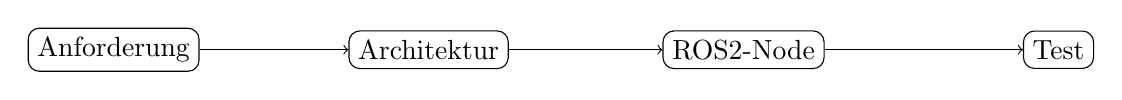
\begin{tikzpicture}[node distance=1.6cm]
\node (req) [draw, rounded corners] {Anforderung};
\node (arch) [draw, rounded corners, right of=req, xshift=2.4cm] {Architektur};
\node (impl) [draw, rounded corners, right of=arch, xshift=2.4cm] {ROS2-Node};
\node (test) [draw, rounded corners, right of=impl, xshift=2.4cm] {Test};
\draw[->] (req) -- (arch);
\draw[->] (arch) -- (impl);
\draw[->] (impl) -- (test);
\end{tikzpicture}
\end{center}

\section{Grenzen von MBSE}
MBSE löst keine schlechten technischen Entscheidungen. Ein Modell kann falsch, veraltet oder unnötig kompliziert sein. Der Nutzen entsteht nur, wenn das Modell gepflegt wird und echte Entscheidungen unterstützt.

\begin{uebungbox}
Erstellen Sie eine Tabelle mit drei Spalten: Information, klassischer Speicherort und Speicherort im MBSE-Modell. Tragen Sie Anforderungen, Schnittstellen, Tests und ROS2-Nodes ein.
\end{uebungbox}

\chapter{SysML-Grundlagen}

\begin{lernziele}
Nach diesem Kapitel kennen Sie die wichtigsten SysML-Diagrammtypen und wissen, wofür sie eingesetzt werden.
\end{lernziele}

\section{Was ist SysML?}
\gls{sysml} steht für Systems Modeling Language. Die Sprache wurde entwickelt, um technische Systeme modellieren zu können. Sie basiert auf UML, ist aber stärker auf Systeme aus Hardware, Software, Menschen, Prozessen und physikalischen Zusammenhängen ausgerichtet.

\section{Diagrammtypen}
Für den Einstieg sind sechs Diagrammtypen besonders wichtig.

\subsection{Requirement Diagram}
Das Requirement Diagram beschreibt Anforderungen und ihre Beziehungen. Es zeigt, welche Anforderungen voneinander abhängen und welche Elemente sie erfüllen oder verifizieren.

\subsection{Block Definition Diagram}
Das \gls{bdd} beschreibt die Systemstruktur auf einer eher abstrakten Ebene. Es zeigt Blöcke und ihre Beziehungen.

\subsection{Internal Block Diagram}
Das \gls{ibd} zeigt die innere Struktur eines Blocks. Es zeigt Teile, Ports und Verbindungen.

\subsection{Activity Diagram}
Aktivitätsdiagramme beschreiben Abläufe. Sie eignen sich für Prozesse, Algorithmen und Betriebsabläufe.

\subsection{State Machine Diagram}
Zustandsdiagramme beschreiben Zustände und Übergänge. Sie sind besonders nützlich für Systeme mit klaren Betriebsmodi.

\subsection{Parametric Diagram}
Parametrische Diagramme beschreiben mathematische Beziehungen, zum Beispiel Energieverbrauch oder Reichweite.

\section{Nicht alles gleichzeitig lernen}
Einsteiger sollten nicht versuchen, sofort jedes Diagramm perfekt zu beherrschen. Der sinnvolle Einstieg lautet: Anforderungen, BDD, IBD, Aktivitätsdiagramm und Zustandsdiagramm. Parametrik kann später folgen.

\begin{praxisbox}
Für den Indoor-Roboter beginnen wir mit Anforderungen und Struktur. Erst wenn klar ist, was der Roboter können soll und aus welchen Hauptsystemen er besteht, modellieren wir Verhalten und technische Details.
\end{praxisbox}

\section{Modell statt Bild}
Ein SysML-Diagramm ist nur eine Sicht auf ein Modell. Das ist wichtig: Wenn ein Block in mehreren Diagrammen erscheint, ist es derselbe Block. Wird der Name geändert, sollte sich die Änderung überall widerspiegeln. Gute Modellierungswerkzeuge speichern also nicht nur Zeichnungen, sondern Modellinformationen.

\begin{uebungbox}
Ordnen Sie folgende Fragen einem Diagrammtyp zu: Was muss das System leisten? Aus welchen Teilen besteht es? Welche Daten fließen zwischen Komponenten? Welche Zustände kann der Roboter haben?
\end{uebungbox}

\chapter{Werkzeuge für SysML v2 einrichten}

\begin{lernziele}
Nach diesem Kapitel können Sie erklären, warum dieses Lehrbuch eine textuelle SysML-v2-Arbeitsweise verwendet. Sie können ein einfaches Projekt in VS Code mit dem Syside Editor anlegen, SysML-v2-Dateien strukturieren und grafische Sichten als Ergänzung einordnen. Außerdem verstehen Sie, warum ein Werkzeug fachliches Modellieren unterstützt, aber nicht ersetzt.
\end{lernziele}

\section{Einleitung}
SysML v2 kann grafisch und textuell verwendet werden. Für dieses Lehrbuch steht die textuelle Notation im Vordergrund. Das passt gut zu modernen Entwicklungsabläufen: Modelle liegen in Dateien, können versioniert, verglichen, überprüft und gemeinsam mit Code gepflegt werden.

Als kostenloser Einstieg eignet sich der Syside Editor für VS Code. Er unterstützt SysML-v2-Dateien mit Syntaxhervorhebung, Autovervollständigung, Formatierung, Gliederung und Validierung. Für grafische Sichten kann zusätzlich Eclipse SysON genutzt werden. SysON ist ein webbasiertes Open-Source-Werkzeug für SysML-v2-Modelle.

\begin{hinweisbox}
Ein Werkzeug löst keine Modellierungsaufgabe automatisch. Es hilft beim Schreiben, Prüfen und Anzeigen des Modells. Die fachliche Entscheidung bleibt Ihre Aufgabe: Welche Elemente gibt es? Welche Beziehungen sind wichtig? Welche Anforderungen müssen nachverfolgbar sein?
\end{hinweisbox}

\section{Warum textuelle Modellierung?}
Viele Einsteiger erwarten bei SysML zuerst Diagramme. Diagramme bleiben wichtig, aber SysML v2 macht den Modellinhalt stärker als präzisen Text zugänglich. Ein Modell kann dadurch ähnlich behandelt werden wie Quellcode.

Textuelle Modellierung hat mehrere Vorteile:

\begin{itemize}
    \item Modelle lassen sich in Git versionieren.
    \item Änderungen sind als Textvergleich sichtbar.
    \item Beispiele können direkt im Lehrbuch gezeigt werden.
    \item Modellteile können leichter wiederverwendet werden.
    \item Validierung und Automatisierung werden einfacher.
    \item ROS2-Code und SysML-v2-Modell können im selben Projekt liegen.
\end{itemize}

Das bedeutet nicht, dass Diagramme unwichtig werden. Diagramme sind weiterhin wertvolle Sichten. Der Unterschied ist: Das Modell entsteht nicht nur durch Zeichnen, sondern durch präzise definierte Modellelemente.

\section{Empfohlene Werkzeugkette}
Für dieses Lehrbuch verwenden wir eine einfache Werkzeugkette:

\begin{itemize}
    \item VS Code als Editor
    \item Syside Editor als SysML-v2-Erweiterung
    \item Git für Versionsverwaltung
    \item optional Eclipse SysON für grafische Sichten
    \item optional das SysML-v2-Pilotprojekt als Referenz für fortgeschrittene Experimente
\end{itemize}

Diese Auswahl ist bewusst pragmatisch. Sie ist kostenlos zugänglich, passt zu textueller Modellierung und überfordert Einsteiger weniger als große industrielle Modellierungsumgebungen.

\section{Projekt anlegen}
Für das Lehrbuch verwenden wir ein Projekt mit dem Namen \texttt{AutonomousIndoorRobot}. Der Name ist bewusst englisch, weil spätere ROS2-Pakete, Nodes und Topics ebenfalls englische technische Bezeichnungen verwenden. Die erklärenden Texte im Modell können trotzdem deutsch sein.

Eine einfache Projektstruktur kann so aussehen:

\begin{verbatim}
AutonomousIndoorRobot/
  model/
    00_overview.sysml
    01_context.sysml
    02_requirements.sysml
    03_structure.sysml
    04_behavior.sysml
    05_interfaces.sysml
    06_tests.sysml
    07_ros2_mapping.sysml
  code/
    status_node.py
    battery_monitor_node.py
  docs/
    decisions.md
\end{verbatim}

Die Dateien im Ordner \texttt{model} enthalten das SysML-v2-Modell. Der Ordner \texttt{code} enthält spätere ROS2-Beispiele. Der Ordner \texttt{docs} kann kurze Architekturentscheidungen aufnehmen.

\section{Erste SysML-v2-Datei}
Eine erste Datei \texttt{00\_overview.sysml} kann den Projektrahmen beschreiben:

\begin{lstlisting}
package AutonomousIndoorRobot {
  doc
  /* Ein Lernmodell für einen autonomen Indoor-Roboter.
     Das Modell verbindet Anforderungen, Struktur, Verhalten,
     Schnittstellen, ROS2-Mapping und Tests. */

  part def Robot;
}
\end{lstlisting}

Dieses Beispiel ist noch sehr klein. Es zeigt aber bereits eine wichtige Idee: Das System wird nicht als loses Bild begonnen, sondern als benannter Modellraum mit einem ersten Systemelement.

\section{Empfohlene Modellstruktur}
Die Modellstruktur orientiert sich an den wichtigsten Fragen des Projekts:

\begin{itemize}
    \item \texttt{00\_overview.sysml}: Ziel, Umfang und Systemgrenze
    \item \texttt{01\_context.sysml}: Stakeholder, externe Systeme und Umgebung
    \item \texttt{02\_requirements.sysml}: Anforderungen und Beziehungen
    \item \texttt{03\_structure.sysml}: Systemteile, Subsysteme und Komponenten
    \item \texttt{04\_behavior.sysml}: Aktionen, Abläufe und Zustände
    \item \texttt{05\_interfaces.sysml}: Ports, Verbindungen und Datenflüsse
    \item \texttt{06\_tests.sysml}: Testfälle und Verifikation
    \item \texttt{07\_ros2\_mapping.sysml}: Zuordnung zu ROS2-Nodes, Topics, Services und Actions
\end{itemize}

Diese Struktur ist bewusst schlicht. Sie trennt die wichtigsten Modellbereiche, ohne schon zu Beginn ein kompliziertes Metamodell einzuführen.

\section{Namenskonventionen}
Klare Namen machen Modelle lesbar. Für dieses Lehrbuch verwenden wir einfache Regeln:

\begin{itemize}
    \item Packages: \texttt{AutonomousIndoorRobot}
    \item Part Definitions: \texttt{Robot}, \texttt{BatterySystem}, \texttt{NavigationSystem}
    \item Parts: \texttt{batterySystem}, \texttt{navigationSystem}
    \item Actions: \texttt{MonitorBattery}, \texttt{NavigateToGoal}
    \item Requirements: \texttt{REQ\_DetectObstacles}, \texttt{REQ\_ReturnToDock}
    \item Testfälle: \texttt{TC\_BatteryLowReturn}
    \item ROS2-Nodes: \texttt{battery\_monitor\_node}
    \item Topics: \texttt{/battery\_state}, \texttt{/cmd\_vel}
\end{itemize}

Vermeiden Sie wechselnde Namen für dasselbe Element. Wenn ein Element einmal \texttt{BatterySystem} heißt, sollte es nicht an anderer Stelle \texttt{PowerModule} genannt werden, außer Sie modellieren bewusst unterschiedliche Dinge.

\section{Grafische Sichten}
Grafische Sichten sind besonders hilfreich, wenn ein Team schnell über Struktur oder Schnittstellen sprechen möchte. In SysML v2 sollte man sie als Darstellung des Modells verstehen, nicht als Ersatz für das Modell.

Eclipse SysON kann für solche Sichten interessant sein. Es ist besonders dann nützlich, wenn Sie aus dem textuellen Modell heraus Struktur-, Verbindungs- oder Anforderungssichten visualisieren wollen. Für den Einstieg in diesem Buch reicht es aber, zunächst die textuelle Notation sauber zu verstehen.

\section{Typische Anfängerfehler}
\subsection{Text wie Programmcode ohne Bedeutung schreiben}
SysML-v2-Text sieht teilweise wie Code aus. Trotzdem modellieren Sie kein Programm, sondern ein System. Fragen Sie bei jedem Element: Welche fachliche Aussage steckt dahinter?

\subsection{Zu früh zu viele Dateien anlegen}
Eine klare Struktur hilft, aber zu viele leere Dateien machen den Einstieg schwer. Beginnen Sie mit Überblick, Anforderungen und Struktur. Verhalten, Tests und Mapping können anschließend wachsen.

\subsection{Diagramme als Wahrheit behandeln}
Ein Diagramm zeigt nur eine Sicht. Die eigentliche Wahrheit liegt im Modell und seinen Beziehungen. Wenn Diagramm und Modell auseinanderlaufen, muss das Modell geklärt werden.

\subsection{Werkzeugvalidierung mit Modellqualität verwechseln}
Ein syntaktisch gültiges Modell kann fachlich trotzdem schlecht sein. Validierung findet Schreibfehler und Regelverstöße, aber keine unklare Systemgrenze oder fehlende Sicherheitsanforderung.

\section{Zusammenfassung}
Dieses Lehrbuch verwendet SysML v2 textuell und einsteigerfreundlich. VS Code mit dem Syside Editor ist die empfohlene kostenlose Arbeitsumgebung. Eclipse SysON kann grafische Sichten ergänzen. Entscheidend bleibt aber nicht das Werkzeug, sondern ein verständliches, konsistentes und nachverfolgbares Modell.

\section{Kontrollfragen}
\begin{enumerate}
    \item Warum eignet sich textuelle Modellierung gut für SysML v2?
    \item Welche Rolle spielt der Syside Editor in diesem Lehrbuch?
    \item Warum sind grafische Sichten trotzdem nützlich?
    \item Welche Dateien enthält die empfohlene Modellstruktur?
    \item Warum sollten Modellelemente einheitlich benannt werden?
    \item Warum ersetzt Werkzeugvalidierung keine fachliche Modellprüfung?
\end{enumerate}

\section{Übungen}
\begin{uebungbox}
\textbf{Übung 1: Projektstruktur anlegen}\\
Legen Sie die empfohlene Ordnerstruktur für \texttt{AutonomousIndoorRobot} an. Erstellen Sie eine Datei \texttt{00\_overview.sysml} und beschreiben Sie Ziel, Umfang und Systemgrenze des Roboterprojekts.
\end{uebungbox}

\begin{uebungbox}
\textbf{Übung 2: Namensregeln anwenden}\\
Formulieren Sie Namen für fünf Anforderungen, drei Testfälle, fünf Part Definitions und vier ROS2-Topics. Achten Sie auf einheitliche Schreibweise.
\end{uebungbox}

\begin{uebungbox}
\textbf{Übung 3: Sicht statt Wahrheit}\\
Beschreiben Sie in drei Sätzen, warum ein Diagramm in SysML v2 nur eine Sicht auf das Modell ist.
\end{uebungbox}

\section{Literaturhinweise}
Für die praktische Arbeit mit SysML v2 sind die Dokumentation des Syside Editors, das Eclipse-SysON-Projekt und das SysML-v2-Pilotprojekt hilfreich \cite{syside,syson,sysmlv2pilot}. Für die fachliche Einordnung bleiben klassische SysML- und MBSE-Grundlagen nützlich, müssen aber bewusst auf SysML v2 übertragen werden.

\chapter{Das Praxisprojekt: Autonomer Indoor-Roboter}

\begin{lernziele}
Nach diesem Kapitel kennen Sie das Beispielsystem, seine Hauptfunktionen und die wichtigsten Randbedingungen.
\end{lernziele}

\section{Ziel des Systems}
Der autonome Indoor-Roboter soll sich in Innenräumen bewegen, Hindernisse erkennen, Personen erkennen, Ziele anfahren und bei niedrigem Akkustand zur Ladestation zurückkehren.

\section{Warum dieses Beispiel?}
Das Beispiel verbindet mehrere typische Bereiche moderner Systementwicklung: Sensorik, Aktorik, Software, Datenverarbeitung, Robotik, künstliche Intelligenz und Tests. Es ist komplex genug, damit SysML Sinn ergibt, aber nicht so groß, dass Einsteiger den Überblick verlieren.

\section{Hauptfunktionen}
\begin{itemize}
\item Umgebung erfassen
\item Karte erstellen oder laden
\item Position bestimmen
\item Navigationsziel empfangen
\item Pfad planen
\item Hindernissen ausweichen
\item Personen erkennen
\item Batterie überwachen
\item Ladestation anfahren
\end{itemize}

\section{Systemkontext}
Der Roboter interagiert mit Nutzern, Räumen, Hindernissen, Ladestation und Wartungspersonal. Diese externen Elemente gehören nicht alle zwingend zum System, beeinflussen aber Anforderungen und Schnittstellen.

\section{Annahmen}
Für dieses Lehrbuch nehmen wir an, dass der Roboter mit Kamera, Lidar, mobilem Rechner, Motorcontroller und Batterie ausgestattet ist. Als Softwarebasis verwenden wir ROS2. Für die Personenerkennung wird später ein ML-Modell eingebunden.

\begin{hinweisbox}
Das Projekt ist didaktisch vereinfacht. Ein echter sicherheitskritischer Roboter würde zusätzliche Sicherheitsanalysen, Normenbetrachtungen und Zulassungsprozesse benötigen.
\end{hinweisbox}

\begin{uebungbox}
Zeichnen Sie eine einfache Kontextskizze: Roboter in der Mitte, außen Nutzer, Hindernis, Ladestation, Raum und Wartungstechniker.
\end{uebungbox}

\chapter{Anforderungen modellieren}

\begin{lernziele}
Nach diesem Kapitel können Sie Anforderungen verständlich, eindeutig und prüfbar formulieren. Sie können Anforderungen nummerieren, strukturieren, in funktionale und nicht-funktionale Anforderungen unterscheiden und mit SysML-Beziehungen verbinden. Außerdem verstehen Sie, wie Anforderungen im Roboterprojekt von Stakeholderbedürfnissen bis zu Testfällen nachverfolgt werden.
\end{lernziele}

\section{Einleitung}
Anforderungen sind eine der wichtigsten Grundlagen eines Systemmodells. Sie beschreiben, was das System leisten muss und unter welchen Bedingungen es dies tun soll. Ohne gute Anforderungen ist unklar, welche Architektur sinnvoll ist und woran der Projekterfolg gemessen wird.

Beim autonomen Indoor-Roboter klingen viele Wünsche zunächst einfach: Der Roboter soll sicher fahren, Hindernisse erkennen, Personen erkennen, lange genug fahren und leicht bedienbar sein. Für die Entwicklung reicht das nicht. Solche Wünsche müssen in Anforderungen übersetzt werden, die eindeutig und später überprüfbar sind.

\section{Was ist eine gute Anforderung?}
Eine gute Anforderung ist:

\begin{itemize}
    \item verständlich
    \item eindeutig
    \item notwendig
    \item realistisch
    \item prüfbar
    \item möglichst lösungsneutral
\end{itemize}

\enquote{Der Roboter soll gut navigieren} ist keine gute Anforderung. Was bedeutet \enquote{gut}? Schnell? Genau? Sicher? Ohne Kollision? In unbekannten Räumen? Eine bessere Formulierung lautet:

\begin{quote}
Der Roboter muss in einem bekannten Innenraum ein ausgewähltes Ziel autonom anfahren und dabei statische Hindernisse im Fahrweg vermeiden.
\end{quote}

Auch diese Anforderung kann später noch präziser werden, aber sie ist deutlich verständlicher.

\section{Vom Bedürfnis zur Anforderung}
Stakeholder äußern häufig Bedürfnisse. Diese Bedürfnisse sind wichtig, aber noch keine technischen Anforderungen.

\begin{center}
\begin{tabular}{p{0.38\textwidth}p{0.50\textwidth}}
\toprule
\textbf{Bedürfnis} & \textbf{Mögliche Anforderung} \\
\midrule
Der Roboter soll niemanden gefährden. & Der Roboter muss bei einem Hindernis im Abstand von 0,5 m seine Geschwindigkeit reduzieren und bei 0,2 m stoppen. \\
Der Roboter soll einfach bedienbar sein. & Ein Transportauftrag muss mit höchstens drei Eingaben gestartet werden können. \\
Der Roboter soll nicht liegen bleiben. & Der Roboter muss bei niedrigem Akkustand automatisch zur Ladestation zurückkehren. \\
Wartung soll einfach sein. & Der Roboter muss Sensorstatus, Akkustatus und Fehlermeldungen anzeigen. \\
\bottomrule
\end{tabular}
\end{center}

\section{Beispielanforderungen}
\begin{longtable}{p{0.16\textwidth}p{0.69\textwidth}}
\toprule
ID & Anforderung\\
\midrule
REQ-001 & Der Roboter muss autonom in einem bekannten Innenraumbereich navigieren können.\\
REQ-002 & Der Roboter muss Hindernisse im Fahrbereich erkennen.\\
REQ-003 & Der Roboter muss erkannte Hindernisse umfahren oder rechtzeitig stoppen.\\
REQ-004 & Der Roboter muss Personen im Kamerabild erkennen können.\\
REQ-005 & Der Roboter muss seinen Akkustand überwachen.\\
REQ-006 & Der Roboter muss bei niedrigem Akkustand selbstständig zur Ladestation fahren.\\
REQ-007 & Der Roboter muss seinen Betriebszustand melden.\\
REQ-008 & Der Roboter muss einen sicheren Zustand einnehmen, wenn ein kritischer Sensor ausfällt.\\
REQ-009 & Der Roboter muss Transportaufträge über eine einfache Benutzerschnittstelle entgegennehmen.\\
REQ-010 & Der Roboter muss relevante Fehler für Wartungspersonal nachvollziehbar protokollieren.\\
\bottomrule
\end{longtable}

\section{Funktionale und nicht-funktionale Anforderungen}
Funktionale Anforderungen beschreiben, was das System tun soll. Beispiele sind Navigation, Hinderniserkennung, Akkustandsüberwachung oder Statusmeldung.

Nicht-funktionale Anforderungen beschreiben Eigenschaften des Systems. Beispiele sind Geschwindigkeit, Genauigkeit, Verfügbarkeit, Sicherheit, Wartbarkeit, Datenschutz oder Energieverbrauch.

Beide Arten sind wichtig. Ein Roboter, der alle Funktionen besitzt, aber zu langsam, unsicher oder unwartbar ist, erfüllt das Projektziel nicht.

\section{Anforderungen strukturieren}
In größeren Projekten werden Anforderungen hierarchisch strukturiert. Eine oberste Anforderung kann in mehrere konkrete Anforderungen zerlegt werden.

Beispiel:

\begin{itemize}
    \item REQ-SAFE-001: Der Roboter muss sicher in der Nähe von Menschen betrieben werden.
    \item REQ-SAFE-002: Der Roboter muss Hindernisse im Fahrweg erkennen.
    \item REQ-SAFE-003: Der Roboter muss bei Gefahr stoppen.
    \item REQ-SAFE-004: Der Roboter muss bei Sensorausfall einen sicheren Zustand einnehmen.
\end{itemize}

Die allgemeine Sicherheitsanforderung wird dadurch handhabbarer.

\section{SysML-Beziehungen}
Wichtige Beziehungen in SysML sind:

\begin{itemize}
    \item \texttt{derive}: Eine Anforderung wird aus einer anderen abgeleitet.
    \item \texttt{satisfy}: Ein Modellelement erfüllt eine Anforderung.
    \item \texttt{verify}: Ein Testfall überprüft eine Anforderung.
    \item \texttt{trace}: Eine allgemeine Nachverfolgungsbeziehung.
    \item \texttt{refine}: Ein Element beschreibt eine Anforderung genauer.
\end{itemize}

\begin{praxisbox}
REQ-002 \enquote{Hindernisse erkennen} wird durch das \texttt{PerceptionSystem} erfüllt. Der Testfall \texttt{TC-002 Hinderniserkennung} verifiziert diese Anforderung. Eine \texttt{trace}-Beziehung kann zusätzlich zeigen, dass der ROS2-Node \texttt{obstacle\_detector\_node} zur Umsetzung gehört.
\end{praxisbox}

Abbildung~\ref{fig:kap06-traceability-req002} stellt diese Traceability-Kette grafisch dar: \texttt{satisfy} und \texttt{verify} zeigen als zwei getrennte, eingehende Beziehungen auf das \texttt{PerceptionSystem}, von dort führt \texttt{trace} weiter zum ROS2-Node.

\begin{figure}[H]
  \centering
  \adjustbox{max width=\linewidth,max totalheight=0.6\textheight}{% =====================================================================
% Abbildung: Traceability-Kette am Beispiel REQ-002
% Passend zu Kapitel 6, Abschnitt "SysML-Beziehungen"
%
% Einbindung im Buch, z. B. in chapters/06_anforderungen.tex:
%
%   \begin{figure}[H]
%     \centering
%     % =====================================================================
% Abbildung: Traceability-Kette am Beispiel REQ-002
% Passend zu Kapitel 6, Abschnitt "SysML-Beziehungen"
%
% Einbindung im Buch, z. B. in chapters/06_anforderungen.tex:
%
%   \begin{figure}[H]
%     \centering
%     \input{figures/fig_kap06_traceability_req002}
%     \caption{Traceability-Kette von REQ-002 ueber \texttt{satisfy} und
%       \texttt{verify} zum \texttt{PerceptionSystem} und per \texttt{trace}
%       weiter zum ROS2-Node.}
%     \label{fig:kap06-traceability-req002}
%   \end{figure}
%
% Benoetigte Pakete (im Buch bereits in main.tex geladen): tikz
% Benoetigte TikZ-Bibliotheken: positioning, arrows.meta, shadows, calc
% =====================================================================

\input{figures/fig_kap06_traceability_req002.tikz}

%     \caption{Traceability-Kette von REQ-002 ueber \texttt{satisfy} und
%       \texttt{verify} zum \texttt{PerceptionSystem} und per \texttt{trace}
%       weiter zum ROS2-Node.}
%     \label{fig:kap06-traceability-req002}
%   \end{figure}
%
% Benoetigte Pakete (im Buch bereits in main.tex geladen): tikz
% Benoetigte TikZ-Bibliotheken: positioning, arrows.meta, shadows, calc
% =====================================================================

\begin{tikzpicture}[
    every node/.style={font=\small},
    req/.style={
        rectangle, rounded corners=1.5pt, draw=black!70, thick,
        minimum width=34mm, minimum height=12mm,
        align=center, fill=blue!12, drop shadow
    },
    part/.style={
        rectangle, rounded corners=1.5pt, draw=green!40!black, thick,
        minimum width=34mm, minimum height=12mm,
        align=center, fill=green!15, drop shadow
    },
    test/.style={
        rectangle, rounded corners=1.5pt, draw=black!50, thick,
        minimum width=34mm, minimum height=12mm,
        align=center, fill=black!6, drop shadow
    },
    code/.style={
        rectangle, rounded corners=1.5pt, draw=orange!60!black, thick,
        minimum width=40mm, minimum height=12mm,
        align=center, fill=orange!15, drop shadow
    },
    flow/.style={-{Stealth[length=2.2mm]}, thick, black!60},
    lbl/.style={font=\small, fill=white, inner sep=1pt}
]

% --- Knoten ---
\node[req]  (req002)  at (0, 3)     {\texttt{REQ-002}\\Hindernisse erkennen};
\node[part] (percept) at (7, 3)     {\texttt{PerceptionSystem}};
\node[test] (tc002)   at (0, -1.5)  {\texttt{TC-002}\\Hinderniserkennung};
\node[code] (rosnode) at (7, -1.5)  {\texttt{obstacle\_detector\_node}};

% --- Beziehungen ---
\draw[flow] (req002) -- node[lbl, midway]{\texttt{satisfy}} (percept);
\draw[flow] (tc002)  to[bend left=12] node[lbl, near end]{\texttt{verify}} (percept);
\draw[flow] (percept) -- node[lbl, midway]{\texttt{trace}} (rosnode);

% --- Legende ---
\node[req,  minimum width=6mm, minimum height=4mm, below=15mm of tc002, xshift=-8mm, font=\tiny] (leg1) {};
\node[right=1mm of leg1, font=\tiny, align=left] {Anforderung};
\node[part, minimum width=6mm, minimum height=4mm, below=6mm of leg1, font=\tiny] (leg2) {};
\node[right=1mm of leg2, font=\tiny, align=left] {Systemteil (\texttt{part def})};
\node[test, minimum width=6mm, minimum height=4mm, below=6mm of leg2, font=\tiny] (leg3) {};
\node[right=1mm of leg3, font=\tiny, align=left] {Testfall};
\node[code, minimum width=6mm, minimum height=4mm, below=6mm of leg3, font=\tiny] (leg4) {};
\node[right=1mm of leg4, font=\tiny, align=left] {ROS2-Node};

\end{tikzpicture}

}
  \caption{Traceability-Kette von REQ-002 über \texttt{satisfy} und \texttt{verify} zum \texttt{PerceptionSystem} und per \texttt{trace} weiter zum ROS2-Node.}
  \label{fig:kap06-traceability-req002}
\end{figure}

\section{Anforderungen in SysML v2}
In SysML v2 werden Anforderungen – eingebettet in ein \texttt{package} wie bereits aus Kapitel 3 bekannt – textuell mit dem Schlüsselwort \texttt{requirement} definiert:

\begin{lstlisting}
package Requirements {

  requirement REQ_001 {
    doc /* Der Roboter muss in einem bekannten Innenraumbereich
           autonom navigieren koennen. */
  }

  requirement REQ_SAFE {
    doc /* Sicherheitsanforderungen. */
    requirement REQ_SAFE_001 {
      doc /* Der Roboter muss Hindernisse im Fahrweg erkennen. */
      derive REQ_001;
    }
  }
}
\end{lstlisting}

Anders als bei \texttt{part def} und \texttt{part} in Kapitel 8 unterscheidet SysML v2 bei \texttt{requirement} im Grundfall nicht zwischen Typ und Nutzung: Das Schlüsselwort \texttt{requirement} definiert die Anforderung im Beispiel gleichzeitig als solche.

Erstellen Sie in der Datei \texttt{02\_requirements.sysml} erste Requirement-Elemente. Verwenden Sie klare Namen, eine stabile ID und einen prüfbaren Text. Achten Sie darauf, dass Anforderungen nicht nur als Liste existieren, sondern später mit Systemteilen, Verhalten und Tests verbunden werden.

Nutzen Sie Beschreibungsfelder (\texttt{doc /* ... */}), um Annahmen, Begründungen oder offene Fragen zu dokumentieren. Wenn eine Anforderung noch unklar ist, markieren Sie sie bewusst, statt sie stillschweigend als fertig zu behandeln – zum Beispiel mit einem kurzen \texttt{doc /* TBD: ... */}-Vermerk im betroffenen Requirement-Element.

\section{Typische Fehler}
\subsection{Zu allgemeine Anforderungen}
\enquote{Der Roboter soll zuverlässig sein} ist nicht prüfbar. Besser sind konkrete Kriterien.

\subsection{Lösungen als Anforderungen}
\enquote{Der Roboter muss Sensor X verwenden} ist häufig bereits eine Designentscheidung. Besser ist eine lösungsneutrale Fähigkeit, sofern kein konkreter Sensor vorgeschrieben ist.

\subsection{Keine Akzeptanzkriterien}
Eine Anforderung sollte erkennen lassen, wie sie später geprüft wird. Ein Akzeptanzkriterium legt fest, woran sich die Erfüllung konkret zeigt, zum Beispiel: \enquote{Testfall: Bei einem simulierten Hindernis in 0,5\,m Abstand muss die Geschwindigkeit innerhalb 1\,s reduziert werden.} Ohne solche Kriterien entstehen Diskussionen am Projektende.

\subsection{Keine Pflege}
Anforderungen ändern sich. Wichtig ist, Änderungen nachvollziehbar zu halten und betroffene Modellelemente zu prüfen.

\section{Vertiefungsbeispiel: Batteriemanagement mit abgesicherter Rückkehr}
\label{sec:bm-anforderungen}
Die Anforderungen REQ-005 und REQ-006 beschreiben zunächst Akkustandsüberwachung und Rückkehr bei niedrigem Akkustand. Wir verfeinern diese Ausgangslage: Der Roboter soll anhand des bisherigen Verbrauchs abschätzen, ob er den laufenden Transportauftrag noch abschließen und anschließend zur Ladestation zurückkehren kann. Ein fester Akkuschwellwert allein beantwortet diese Frage nicht.

Dieses Beispiel ist ein fachlicher Entwurf. Die folgenden BM-Anforderungen ergänzen die bisherigen Lehrbuchbeispiele; ihre Umsetzung in SysML und ROS2 sowie der Nachweis am Roboter stehen noch aus. Der Entscheidungsablauf folgt in Abschnitt~\ref{sec:bm-ablauf}, die Energiebilanz in Abschnitt~\ref{sec:bm-energie} und die Testzuordnung in Abschnitt~\ref{sec:bm-tests}.

\subsection{Systemgrenze und Annahmen}
Betrachtet werden Akkuzustand, Verbrauchserfassung, Energiebedarfsschätzung, Rückwegabsicherung, Auftragsentscheidung, Navigation und Statusmeldungen. Die Ladestation ist ein externes System. Die Rückkehr endet erst mit bestätigtem Andocken und Ladebeginn.

Als Entwurfsannahme beginnt die Fahrt an einer bekannten Ladestation. Der Roboter zeichnet den gefahrenen Weg und dessen Energieverbrauch auf und kann dem Weg zurück folgen. Diese vorgeschlagenen Fähigkeiten müssen technisch geprüft werden. Ein bereits gefahrener Weg ist weder automatisch in Gegenrichtung befahrbar noch dauerhaft frei. Auch der Rückwegverbrauch darf nicht ungeprüft mit dem Hinwegverbrauch gleichgesetzt werden.

Ein \emph{abgesicherter Rückweg} besitzt einen bekannten Verlauf, ist ausreichend zuverlässig verfolgbar und wurde hinsichtlich Befahrbarkeit und Energiebedarf einschließlich Andocken bewertet. Eine \emph{belastbare Schätzung} verwendet gültige Eingangsdaten und berücksichtigt ihre Unsicherheit. Welche Qualität hierfür genügt, bleibt ein offener Projektparameter.

\begin{hinweisbox}
Sind Restauftrag oder vorgesehener Rückweg nicht abschätzbar, etwa wegen fehlender Kartendaten, darf der Auftrag nicht fortgesetzt werden. Die Rückkehr muss dann durch eine unabhängig abgesicherte Möglichkeit gewährleistet werden, beispielsweise durch eine geeignete Wegaufzeichnung. Eine fehlende Schätzung ist kein geringer Energiebedarf.
\end{hinweisbox}

\subsection{Anforderungen des Vertiefungsbeispiels}
Die IDs BM-01 bis BM-13 bleiben über Anforderungen, Ablauf und Tests hinweg stabil. BM-06 legt bewusst eine Entwurfsentscheidung für dieses Beispiel fest; eine andere technische Rückkehrstrategie wäre gesondert zu bewerten.

\begin{description}[style=nextline]
    \item[BM-01: Startfreigabe] Vor Fahrtbeginn muss der Roboter gültige Akkudaten, Verbrauchserfassung und eine verfügbare Rückkehrstrategie prüfen. Fehlt eine Voraussetzung, darf kein Transportauftrag starten.
    \item[BM-02: Verbrauchsbasierte Schätzung] Der Roboter muss den bisherigen Energieverbrauch erfassen und damit den geschätzten Bedarf aktualisieren. Veränderungen von Last, Fahrprofil oder Umgebung müssen in die Bewertung eingehen.
    \item[BM-03: Entscheidungsgrundlage] Für jede Auftragsentscheidung muss der Roboter nutzbare Restenergie, Bedarf des Restauftrags, anschließenden Rückkehrbedarf und Reserve mit Gültigkeit und Unsicherheit bewerten. Unbekannte Werte dürfen nicht als null gelten.
    \item[BM-04: Auftrag fortsetzen] Der Roboter darf den Auftrag nur fortsetzen, wenn Restauftrag, anschließende Rückkehr und Reserve durch eine belastbare Energieschätzung gedeckt sind. Zusätzlich muss eine Rückkehr vom aktuellen Standort abgesichert bleiben.
    \item[BM-05: Fehlende Abschätzbarkeit] Sind Restauftrag oder anschließender Rückweg nicht abschätzbar, muss der Roboter den Auftrag kontrolliert unterbrechen und eine abgesicherte Rückkehr beginnen. Ein hoher Akkustand hebt diese Regel nicht auf.
    \item[BM-06: Wegaufzeichnung] Der Roboter muss den gefahrenen Weg und zugehörige Verbrauchsdaten für die Rückkehrbewertung aufzeichnen. Lücken und ungültige Abschnitte müssen erkannt und berücksichtigt werden.
    \item[BM-07: Rückwegfreigabe] Ein aufgezeichneter Weg darf nur bei bewerteter Verfolgbarkeit, Befahrbarkeit und ausreichender Energie einschließlich Reserve als abgesicherter Rückweg verwendet werden. Die Aufzeichnung allein genügt nicht.
    \item[BM-08: Laufende Absicherung] Der Roboter muss die Rückkehrabsicherung regelmäßig und bei relevanten Änderungen erneut bewerten. Droht sie verloren zu gehen, muss er die Rückkehr vor Unterschreiten der festgelegten Rückkehrgrenze einleiten. Reaktions- und Unterbrechungszeit sind zu berücksichtigen.
    \item[BM-09: Blockierter Rückweg] Bei einer Blockade muss der Roboter einen alternativen Rückweg bewerten. Er darf ihn nur bei abgesicherter Befahrbarkeit und ausreichender Energie nutzen. Auch Warte- und Planungsenergie müssen berücksichtigt werden.
    \item[BM-10: Keine abgesicherte Rückkehr] Ist kein abgesicherter Rückweg verfügbar, muss der Roboter kontrolliert anhalten und Unterstützung anfordern. Der Auftrag bleibt unterbrochen; die autonome Rückkehr muss als nicht erfüllt gemeldet werden.
    \item[BM-11: Datenausfall] Bei Ausfall von Akkudaten oder Wegaufzeichnung muss der Roboter die verbleibende Rückkehrabsicherung neu bewerten. Nur eine weiterhin belastbar abgesicherte Rückkehr darf fortgesetzt werden; andernfalls gilt BM-10.
    \item[BM-12: Nachvollziehbarer Status] Der Roboter muss Entscheidung, Entscheidungsgrund, Auftragsstatus und Rückkehrstatus nachvollziehbar melden. Fortsetzung, Unterbrechung, Rückkehr und Unterstützungsbedarf müssen unterscheidbar sein.
    \item[BM-13: Rückkehr erfolgreich] Der Roboter darf die Rückkehr erst nach bestätigtem Andocken und Ladebeginn als erfolgreich melden. Das Erreichen der Stationsposition allein genügt nicht.
\end{description}

\subsection{Offene Parameter und Nachweisgrenzen}
Vor einer Implementierung müssen das Verfahren zur Restenergieschätzung, Energiereserve, zulässige Schätzunsicherheit, Rückkehrgrenze, Prüfabstände und Kriterien für gültige Wegdaten festgelegt werden. Ebenso ist zu klären, wie ein kontrolliertes Anhalten bei der vorgesehenen Ladung und Umgebung aussieht. Konkrete Werte werden hier bewusst nicht erfunden.

Damit liegt noch keine technische Rückkehrgarantie vor. Insbesondere die Rückkehr ohne Karte, die Verbrauchsschätzung und unerwartete Wegblockaden benötigen einen Nachweis. Kontrolliertes Anhalten mit Unterstützungsanforderung begrenzt die Folgen eines Fehlers, erfüllt aber nicht die geforderte autonome Rückkehr.

\section{Zusammenfassung}
Anforderungen verbinden Stakeholderbedürfnisse mit Architektur und Tests. Gute Anforderungen sind verständlich, eindeutig und prüfbar. In SysML v2 werden Anforderungen nicht nur gesammelt, sondern über Beziehungen mit Systemteilen, Aktionen, Schnittstellen und Testfällen verbunden.

\section{Kontrollfragen}
\begin{enumerate}
    \item Was macht eine gute Anforderung aus?
    \item Warum ist \enquote{Der Roboter soll gut navigieren} problematisch?
    \item Was ist der Unterschied zwischen funktionalen und nicht-funktionalen Anforderungen?
    \item Wozu dient \texttt{derive}?
    \item Wozu dient \texttt{satisfy}?
    \item Wozu dient \texttt{verify}?
    \item Warum sollten Anforderungen möglichst lösungsneutral sein?
    \item Welche Anforderung könnte aus dem Bedürfnis \enquote{Wartung soll einfach sein} entstehen?
\end{enumerate}

\section{Übungen}
\begin{uebungbox}
\textbf{Übung 1: Anforderungen formulieren}\\
Formulieren Sie fünf zusätzliche Anforderungen: zwei zur Sicherheit, eine zur Bedienung, eine zur Wartung und eine zur Leistung.
\end{uebungbox}

\begin{uebungbox}
\textbf{Übung 2: Anforderungen verbessern}\\
Verbessern Sie die Aussagen \enquote{Der Roboter soll schnell sein}, \enquote{Der Roboter soll zuverlässig sein} und \enquote{Die Bedienung soll intuitiv sein}, sodass daraus prüfbare Anforderungen werden.
\end{uebungbox}

\begin{uebungbox}
\textbf{Übung 3: Beziehungen anlegen}\\
Wählen Sie drei Anforderungen aus der Tabelle. Ordnen Sie jeder Anforderung ein Systemelement (\texttt{part def}) und einen Testfall zu.
\end{uebungbox}

\section{Literaturhinweise}
Anforderungsmodellierung ist ein zentraler Bestandteil von SysML und MBSE. Für den Einstieg eignen sich Delligatti \cite{delligatti2014} sowie Friedenthal, Moore und Steiner \cite{friedenthal2014}. Für reale Projekte sollte zusätzlich Literatur zum Requirements Engineering genutzt werden.

\chapter{Stakeholder und Use Cases}

\begin{lernziele}
Nach diesem Kapitel können Sie Stakeholder identifizieren und aus typischen Nutzungsszenarien Anforderungen ableiten.
\end{lernziele}

\section{Stakeholder identifizieren}
Stakeholder sind nicht nur Endnutzer. Auch Betreiber, Wartung, Entwicklung, Management und Sicherheitsverantwortliche haben Interessen. Ein Roboter, der technisch funktioniert, aber schlecht wartbar ist, kann im Betrieb trotzdem scheitern.

\section{Stakeholder des Roboters}
\begin{itemize}
\item Nutzer: möchte Ziele einfach vorgeben.
\item Betreiber: möchte zuverlässigen Betrieb.
\item Wartungstechniker: benötigt Diagnoseinformationen.
\item Entwickler: benötigt klare Schnittstellen.
\item Sicherheitsverantwortlicher: achtet auf Risiken.
\end{itemize}

\section{Use Cases}
Use Cases beschreiben, wie ein Akteur mit dem System interagiert. Sie sind keine detaillierten Algorithmen, sondern Nutzungsbeschreibungen.

\section{Beispiel: Ziel anfahren}
\textbf{Akteur:} Nutzer\\
\textbf{Ziel:} Roboter fährt zu einem ausgewählten Zielpunkt.\\
\textbf{Vorbedingung:} Roboter ist eingeschaltet und lokalisiert.\\
\textbf{Ablauf:}
\begin{enumerate}
\item Nutzer wählt Ziel.
\item Roboter prüft Verfügbarkeit der Karte.
\item Roboter plant Pfad.
\item Roboter fährt los.
\item Roboter weicht Hindernissen aus.
\item Roboter erreicht Ziel.
\end{enumerate}

\section{Use Cases und Anforderungen}
Aus einem Use Case lassen sich Anforderungen ableiten. Wenn der Roboter Ziele anfahren soll, braucht er Navigation, Lokalisierung, Pfadplanung und Hindernisvermeidung.

\begin{uebungbox}
Schreiben Sie einen Use Case \enquote{Zur Ladestation zurückkehren}. Leiten Sie daraus mindestens drei Anforderungen ab.
\end{uebungbox}

\chapter{Block Definition Diagram}

\begin{lernziele}
Nach diesem Kapitel können Sie die Hauptstruktur des Roboters als Block Definition Diagram modellieren.
\end{lernziele}

\section{Zweck des BDD}
Das \gls{bdd} zeigt, aus welchen logischen oder physischen Bausteinen ein System besteht. Ein Block kann Hardware, Software, Mensch, Datenobjekt oder abstrakte Funktion darstellen.

\section{Hauptstruktur des Roboters}
\begin{verbatim}
Robot
|- NavigationSystem
|- PerceptionSystem
|- MotionControl
|- BatterySystem
|- CommunicationSystem
|- UserInterface
\end{verbatim}

Diese Darstellung ist noch grob. Sie eignet sich aber hervorragend, um den Systemumfang zu verstehen.

\section{Komposition}
Eine Komposition beschreibt eine starke Teil-Ganzes-Beziehung. Wenn das \texttt{PerceptionSystem} Teil des Roboters ist, kann dies als Komposition modelliert werden.

\section{Dekomposition}
Das \texttt{PerceptionSystem} kann weiter zerlegt werden:
\begin{verbatim}
PerceptionSystem
|- Camera
|- Lidar
|- ObjectDetector
|- ObstacleDetector
\end{verbatim}

\section{Logische und physische Blöcke}
Ein häufiger Anfängerfehler besteht darin, logische Funktionen und physische Bauteile unklar zu vermischen. \texttt{Camera} ist eher physisch. \texttt{ObjectDetector} ist eher logisch oder softwarebezogen. Beides darf im Modell vorkommen, sollte aber bewusst getrennt werden.

\begin{hinweisbox}
Ein BDD muss nicht sofort perfekt sein. Es entwickelt sich mit dem Verständnis des Systems.
\end{hinweisbox}

\begin{uebungbox}
Erstellen Sie ein BDD mit dem Block \texttt{Robot} und mindestens fünf Subsystemen. Ergänzen Sie beim \texttt{PerceptionSystem} Kamera, Lidar und Objekterkennung.
\end{uebungbox}

\chapter{Internal Block Diagram}

\begin{lernziele}
Nach diesem Kapitel können Sie Datenflüsse und interne Verbindungen zwischen Komponenten im IBD darstellen.
\end{lernziele}

\section{Zweck des IBD}
Das \gls{ibd} zeigt, wie Teile eines Blocks intern verbunden sind. Während das BDD sagt, welche Bausteine existieren, zeigt das IBD, wie sie zusammenarbeiten.

\section{Beispiel Datenfluss}
\begin{verbatim}
Camera -> ObjectDetector -> NavigationSystem
Lidar  -> SLAM           -> NavigationSystem
NavigationSystem -> MotionControl -> Motors
BatterySystem -> NavigationSystem
\end{verbatim}

\section{Ports}
Ports beschreiben Ein- und Ausgänge von Blöcken. Ein Kamerablock kann einen Port \texttt{imageOut} haben. Der ObjectDetector kann einen Port \texttt{imageIn} und \texttt{objectsOut} haben.

\section{Schnittstellen}
Eine Verbindung ohne klare Schnittstelle ist wenig wert. Deshalb sollte dokumentiert werden, welche Daten übertragen werden. Beispiel: \texttt{sensor\_msgs/Image} für Kamerabilder in ROS2.

\section{IBD und ROS2}
Das IBD passt gut zur ROS2-Kommunikation. ROS2-Topics können als Datenflüsse modelliert werden. Ein Topic \texttt{/camera/image\_raw} verbindet \texttt{camera\_node} und \texttt{object\_detector\_node}.

\begin{uebungbox}
Erstellen Sie ein IBD für das \texttt{PerceptionSystem}. Modellieren Sie Kamera, Lidar, ObjectDetector und ObstacleDetector inklusive Datenflüssen.
\end{uebungbox}

\chapter{Schnittstellenmodellierung}

\begin{lernziele}
Nach diesem Kapitel können Sie Schnittstellen beschreiben und erkennen, warum klare Schnittstellen in Robotikprojekten entscheidend sind.
\end{lernziele}

\section{Warum Schnittstellen wichtig sind}
Viele technische Probleme entstehen nicht in einzelnen Komponenten, sondern an ihren Schnittstellen. Eine Kamera liefert Bilder in einem Format, das der Erkennungsalgorithmus nicht erwartet. Ein Navigationsknoten erwartet Koordinaten in einem anderen Bezugssystem. Solche Fehler sind typisch.

\section{Schnittstellenbeschreibung}
Eine gute Schnittstellenbeschreibung enthält:
\begin{itemize}
\item Name der Schnittstelle
\item Sender und Empfänger
\item Datentyp
\item Frequenz oder Ereignis
\item Qualitätsanforderungen
\item Fehlerfälle
\end{itemize}

\section{Beispiel}
\begin{longtable}{p{35mm}p{35mm}p{35mm}p{35mm}}
\toprule
Schnittstelle & Sender & Empfänger & Datentyp\\
\midrule
Kamerabild & Camera & ObjectDetector & sensor\_msgs/Image\\
Laserscan & Lidar & SLAM & sensor\_msgs/LaserScan\\
Bewegungsbefehl & Navigation & MotionControl & geometry\_msgs/Twist\\
Akkustatus & BatterySystem & Navigation & sensor\_msgs/BatteryState\\
\bottomrule
\end{longtable}

\section{Koordinatensysteme}
In Robotikprojekten sind Koordinatensysteme kritisch. ROS2 nutzt häufig Frames wie \texttt{map}, \texttt{odom}, \texttt{base\_link} und \texttt{camera\_link}. Diese sollten im Modell dokumentiert werden.

\begin{uebungbox}
Erstellen Sie eine Schnittstellentabelle für mindestens sechs Datenflüsse des Roboters. Ergänzen Sie jeweils Sender, Empfänger und Datentyp.
\end{uebungbox}

\chapter{Verhaltensmodellierung mit Activity Diagrams}

\begin{lernziele}
Nach diesem Kapitel können Sie Abläufe des Roboters als Aktivitätsdiagramm beschreiben.
\end{lernziele}

\section{Was beschreibt ein Aktivitätsdiagramm?}
Ein Aktivitätsdiagramm beschreibt einen Ablauf aus Aktionen, Entscheidungen und Verzweigungen. Es eignet sich gut für Prozesse wie \enquote{Navigationsziel anfahren}.

\section{Beispielablauf Navigation}
\begin{enumerate}
\item System starten
\item Sensoren initialisieren
\item Karte laden
\item Ziel empfangen
\item Pfad planen
\item Bewegung ausführen
\item Hindernisse prüfen
\item Ziel erreicht melden
\end{enumerate}

\section{Entscheidungen}
Entscheidungsknoten modellieren Alternativen. Beispiel: Wenn ein Hindernis erkannt wird, plant der Roboter neu oder stoppt.

\section{Parallelität}
Ein Roboter führt oft mehrere Aktivitäten parallel aus. Während er fährt, überwacht er Sensoren und Batterie. Aktivitätsdiagramme können solche parallelen Abläufe darstellen, sollten am Anfang aber nicht überladen werden.

\begin{praxisbox}
Der Ablauf \enquote{Zur Ladestation fahren} enthält eine Entscheidung: Ist der Akkustand niedrig? Nur dann wird der Ladevorgang gestartet.
\end{praxisbox}

\begin{uebungbox}
Modellieren Sie den Ablauf \enquote{Ziel anfahren}. Ergänzen Sie mindestens eine Entscheidung für Hinderniserkennung und eine für niedrigen Akkustand.
\end{uebungbox}

\chapter{Zustandsmodellierung mit State Machines}

\begin{lernziele}
Nach diesem Kapitel können Sie Betriebszustände und Zustandswechsel eines Roboters modellieren.
\end{lernziele}

\section{Zustände}
Ein Zustand beschreibt eine Situation, in der sich das System über eine gewisse Zeit befindet. Beispiele für den Roboter sind \texttt{Idle}, \texttt{Mapping}, \texttt{Navigation}, \texttt{Charging} und \texttt{Error}.

\section{Ereignisse}
Ereignisse lösen Übergänge aus. Beispiele:
\begin{itemize}
\item \texttt{GoalReceived}
\item \texttt{BatteryLow}
\item \texttt{ObstacleDetected}
\item \texttt{ChargingComplete}
\item \texttt{ErrorDetected}
\end{itemize}

\section{Beispiel}
\begin{verbatim}
Idle --GoalReceived--> Navigation
Navigation --BatteryLow--> ReturnToDock
ReturnToDock --DockReached--> Charging
Charging --ChargingComplete--> Idle
Navigation --ErrorDetected--> Error
\end{verbatim}

\section{Warum State Machines nützlich sind}
Zustandsdiagramme verhindern unklare Logik. Sie zeigen, welche Übergänge erlaubt sind. Darf der Roboter während eines Fehlers ein neues Ziel annehmen? Darf er während des Ladens navigieren? Solche Fragen werden sichtbar.

\begin{uebungbox}
Erstellen Sie eine State Machine für den Roboter mit mindestens fünf Zuständen und acht Übergängen.
\end{uebungbox}

\chapter{Parametrische Modellierung}

\begin{lernziele}
Nach diesem Kapitel verstehen Sie, wie technische Zusammenhänge im Modell beschrieben werden können.
\end{lernziele}

\section{Zweck parametrischer Modelle}
Parametrische Modelle beschreiben mathematische Beziehungen. Sie helfen, technische Entscheidungen zu prüfen. Beim Roboter sind Energieverbrauch, Reichweite und Geschwindigkeit wichtige Größen.

\section{Einfaches Beispiel}
\[
t_{betrieb} = \frac{E_{akku}}{P_{gesamt}}
\]

Dabei ist \(E_{akku}\) die nutzbare Energie der Batterie und \(P_{gesamt}\) die durchschnittliche Leistungsaufnahme.

\section{Leistungsaufnahme}
Die Gesamtleistung kann grob abgeschätzt werden:
\[
P_{gesamt} = P_{rechner} + P_{sensoren} + P_{motoren}
\]

Diese Formel ist einfach, aber nützlich für frühe Architekturentscheidungen.

\section{Parametric Diagram in SysML}
In SysML werden solche Zusammenhänge mit Constraint Blocks modelliert. Ein Constraint Block beschreibt die Formel, Parameter werden mit Systemeigenschaften verbunden.

\begin{hinweisbox}
Parametrik ist für Einsteiger optional. Sie wird wichtig, wenn quantitative Aussagen getroffen werden sollen.
\end{hinweisbox}

\begin{uebungbox}
Nehmen Sie eine Batteriekapazität von 100 Wh und eine Leistungsaufnahme von 25 W an. Berechnen Sie die theoretische Betriebszeit.
\end{uebungbox}

\chapter{ROS2-Grundlagen}

\begin{lernziele}
Nach diesem Kapitel kennen Sie Nodes, Topics, Services und Actions und können diese Begriffe auf das Robotersystem anwenden.
\end{lernziele}

\section{Was ist ROS2?}
\gls{ros2} ist ein Framework für Robotiksoftware. Es stellt Kommunikationsmechanismen, Werkzeuge und Konventionen bereit. ROS2 ist kein Betriebssystem im klassischen Sinn, sondern eine Middleware und Entwicklungsumgebung.

\section{Nodes}
Ein Node ist ein ausführbares Programm mit einer klaren Aufgabe. Beispiel: Ein \texttt{camera\_node} liest Kamerabilder und veröffentlicht sie.

\section{Topics}
Topics sind Nachrichtenkanäle. Ein Node veröffentlicht Nachrichten, andere Nodes abonnieren sie. Diese Publish-Subscribe-Kommunikation passt sehr gut zu Sensordaten.

\section{Services}
Services sind Anfrage-Antwort-Kommunikation. Sie eignen sich für kurze, gezielte Abfragen, zum Beispiel \enquote{Setze Parameter}.

\section{Actions}
Actions sind für länger laufende Aufgaben gedacht. Navigation zu einem Ziel ist ein typischer Action-Anwendungsfall, weil der Vorgang länger dauert und Feedback liefern kann.

\section{Beispiel}
\begin{verbatim}
/camera/image_raw       Kamerabild
/scan                   Laserscan
/cmd_vel                Bewegungsbefehl
/battery_state          Akkustatus
/detected_objects       erkannte Objekte
\end{verbatim}

\begin{uebungbox}
Ordnen Sie den Funktionen Kamera, Navigation, Batterieüberwachung und Objekterkennung passende ROS2-Nodes und Topics zu.
\end{uebungbox}

\chapter{Architektur von ROS2-Systemen}

\begin{lernziele}
Nach diesem Kapitel können Sie eine einfache ROS2-Architektur für den autonomen Roboter entwerfen.
\end{lernziele}

\section{Typische Node-Struktur}
Eine sinnvolle erste Architektur besteht aus folgenden Nodes:
\begin{itemize}
\item \texttt{camera\_node}
\item \texttt{lidar\_node}
\item \texttt{slam\_node}
\item \texttt{navigation\_node}
\item \texttt{object\_detector\_node}
\item \texttt{battery\_monitor\_node}
\item \texttt{motion\_control\_node}
\end{itemize}

\section{Kommunikationsstruktur}
\begin{verbatim}
camera_node -> /camera/image_raw -> object_detector_node
lidar_node  -> /scan             -> slam_node
slam_node   -> /map              -> navigation_node
navigation_node -> /cmd_vel      -> motion_control_node
battery_monitor_node -> /battery_state -> navigation_node
\end{verbatim}

\section{Architekturentscheidungen}
Eine wichtige Entscheidung ist die Granularität. Zu viele Nodes erhöhen Kommunikationsaufwand. Zu wenige Nodes machen das System unübersichtlich. Für den Einstieg gilt: Eine klar abgegrenzte Funktion darf ein eigener Node sein.

\section{Fehlerfälle}
Eine Architektur sollte nicht nur den Normalfall zeigen. Was passiert, wenn die Kamera ausfällt? Was passiert bei leerem Akku? Was passiert, wenn keine Karte verfügbar ist?

\begin{uebungbox}
Erstellen Sie eine ROS2-Architekturskizze mit mindestens sechs Nodes und acht Topics.
\end{uebungbox}

\chapter{Von SysML zu ROS2}

\begin{lernziele}
Nach diesem Kapitel können Sie SysML-Elemente auf ROS2-Elemente abbilden. Sie verstehen, warum Mapping für Traceability wichtig ist und wie Anforderungen, Blöcke, Ports, Datenflüsse und Tests mit Nodes, Topics, Services, Actions und Testcode verbunden werden können.
\end{lernziele}

\section{Einleitung}
Das SysML-Modell beschreibt die Architektur. ROS2 ist die Umsetzung. Ohne Verbindung zwischen beiden entsteht eine Lücke. Das Mapping schließt diese Lücke. Es zeigt, wie Modellentscheidungen in Softwareelemente übersetzt werden.

\section{Grundprinzip}
Ein SysML-Block kann einem ROS2-Node entsprechen. Ein SysML-Port oder Datenfluss kann einem Topic entsprechen. Eine Funktion kann durch einen Node oder eine Gruppe von Nodes realisiert werden. Ein Use Case kann eine Action verwenden. Ein Testfall im Modell kann einem automatisierten Test entsprechen.

\section{Beispieltabelle}
\begin{longtable}{p{45mm}p{45mm}p{45mm}}
\toprule
SysML-Element & ROS2-Element & Bemerkung\\
\midrule
ObjectDetector & \texttt{object\_detector\_node} & Führt ML-Inferenz aus\\
Camera & \texttt{camera\_node} & Liefert Bilddaten\\
NavigationSystem & \texttt{navigation\_node} & Plant und überwacht Bewegung\\
BatterySystem & \texttt{battery\_monitor\_node} & Überwacht Akkustatus\\
MotionControl & \texttt{motion\_control\_node} & Setzt Geschwindigkeitsbefehle um\\
UserInterface & \texttt{user\_interface\_node} & Nimmt Aufträge entgegen\\
\bottomrule
\end{longtable}

\section{Mapping von Schnittstellen}
Ports und Datenflüsse werden auf Topics, Services oder Actions abgebildet:

\begin{itemize}
    \item Bilddaten: \texttt{/camera/image\_raw}
    \item Laserscan: \texttt{/scan}
    \item Bewegungsbefehl: \texttt{/cmd\_vel}
    \item Akkustatus: \texttt{/battery\_state}
    \item Zielnavigation: Action \texttt{NavigateToPose}
\end{itemize}

\section{Traceability}
Das Mapping ist ein Teil der Traceability. Es zeigt, welche Implementierung eine Architekturkomponente realisiert.

\begin{praxisbox}
REQ-004 \enquote{Personen erkennen} wird durch den Block \texttt{ObjectDetector} erfüllt. Dieser Block wird durch den ROS2-Node \texttt{object\_detector\_node} implementiert. Die Ergebnisse werden über \texttt{/detected\_objects} veröffentlicht und durch einen Testfall zur Personenerkennung geprüft.
\end{praxisbox}

\section{Von Anforderungen bis Code}
Eine vollständige Kette kann so aussehen:

\begin{verbatim}
REQ-006 Zur Ladestation zurückkehren
-> Funktion: Akkustand überwachen
-> Block: BatterySystem
-> Node: battery_monitor_node
-> Topic: /battery_state
-> Node: navigation_node
-> Action: NavigateToDock
-> Test: TC-006 Rückkehr bei niedrigem Akkustand
\end{verbatim}

\section{Typische Fehler}
\subsection{Eins-zu-eins-Zwang}
Nicht jeder Block muss genau ein Node werden. Mapping ist eine bewusste Architekturentscheidung.

\subsection{Mapping nicht pflegen}
Wenn sich die ROS2-Architektur ändert, muss das Mapping aktualisiert werden. Sonst verliert die Traceability ihren Wert.

\subsection{Schnittstellen nur grob abbilden}
Ein Mapping ohne Topic-Namen, Nachrichtentypen oder Verantwortlichkeiten ist zu ungenau.

\section{Mapping als lebendes Artefakt}
Das Mapping ist kein einmaliges Abschlussdokument. Es wächst mit dem Projekt. Am Anfang reicht eine grobe Tabelle: Block zu Node, Datenfluss zu Topic. Später kommen Nachrichtentypen, Parameter, Launch-Dateien und Tests hinzu.

Eine gute Mapping-Tabelle kann zusätzliche Spalten enthalten:

\begin{itemize}
    \item SysML-Block
    \item Funktion
    \item ROS2-Node
    \item Topic, Service oder Action
    \item Nachrichtentyp
    \item zugehörige Anforderung
    \item Testfall
    \item Status der Umsetzung
\end{itemize}

Damit wird das Mapping zu einem Arbeitsmittel. Es hilft bei Reviews, bei der Codeplanung und beim Erkennen von Lücken. Wenn ein wichtiger Block keinen Node und keinen Test besitzt, ist das ein Signal für weitere Klärung.

\section{Zusammenfassung}
Das SysML-ROS2-Mapping verbindet Modell und Umsetzung. Es hilft, Anforderungen bis zur Software nachzuverfolgen und Änderungen gezielt zu analysieren. Für dieses Lehrbuch ist es die zentrale Brücke zwischen MBSE und praktischer Robotiksoftware.

\section{Kontrollfragen}
\begin{enumerate}
    \item Warum ist Mapping zwischen SysML und ROS2 wichtig?
    \item Welche SysML-Elemente können auf ROS2-Nodes abgebildet werden?
    \item Welche SysML-Elemente passen zu Topics?
    \item Warum muss Mapping gepflegt werden?
    \item Warum ist ein Eins-zu-eins-Mapping nicht immer sinnvoll?
    \item Erklären Sie eine Traceability-Kette für Batteriemanagement.
\end{enumerate}

\section{Übungen}
\begin{uebungbox}
\textbf{Übung 1: Mapping-Tabelle}\\
Erstellen Sie eine Mapping-Tabelle für alle Hauptblöcke Ihres BDD.
\end{uebungbox}

\begin{uebungbox}
\textbf{Übung 2: Vollständige Kette}\\
Erstellen Sie eine Kette von einer Anforderung über Block, Node, Topic und Testfall für die Hinderniserkennung.
\end{uebungbox}

\section{Literaturhinweise}
Das Mapping verbindet SysML-Grundlagen \cite{delligatti2014,friedenthal2014} mit ROS2-Kommunikation \cite{ros2docs}. In realen Projekten wird diese Verbindung oft projektspezifisch definiert.

\chapter{ROS2-Implementierung mit Python}

\begin{lernziele}
Nach diesem Kapitel verstehen Sie den Aufbau eines einfachen ROS2-Python-Nodes.
\end{lernziele}

\section{Package erstellen}
Ein Python-Package wird typischerweise mit folgendem Befehl erstellt:

\begin{lstlisting}[language=bash]
ros2 pkg create robot_basic_nodes --build-type ament_python --dependencies rclpy std_msgs sensor_msgs geometry_msgs
\end{lstlisting}

\section{Ein einfacher Node}
\begin{lstlisting}[language=Python]
import rclpy
from rclpy.node import Node
from std_msgs.msg import String

class StatusNode(Node):
    def __init__(self):
        super().__init__('status_node')
        self.publisher = self.create_publisher(String, '/robot/status', 10)
        self.timer = self.create_timer(1.0, self.publish_status)

    def publish_status(self):
        msg = String()
        msg.data = 'Robot is running'
        self.publisher.publish(msg)

def main():
    rclpy.init()
    node = StatusNode()
    rclpy.spin(node)
    node.destroy_node()
    rclpy.shutdown()
\end{lstlisting}

\section{Subscriber}
Ein Subscriber empfängt Nachrichten von einem Topic. Der ObjectDetector würde zum Beispiel \texttt{/camera/image\_raw} abonnieren.

\section{Build und Start}
\begin{lstlisting}[language=bash]
colcon build
source install/setup.bash
ros2 run robot_basic_nodes status_node
\end{lstlisting}

\begin{hinweisbox}
Der Code ist bewusst minimal. In realen Projekten kommen Fehlerbehandlung, Parameter, Logging und Launch-Dateien hinzu.
\end{hinweisbox}

\begin{uebungbox}
Implementieren Sie einen \texttt{battery\_monitor\_node}, der regelmäßig einen simulierten Akkustand veröffentlicht.
\end{uebungbox}

\chapter{Machine Learning in ROS2 integrieren}

\begin{lernziele}
Nach diesem Kapitel verstehen Sie, wie ein ML-Modell als ROS2-Node in eine Roboterarchitektur eingebunden wird. Sie können Datenfluss, Inferenz, Ergebnisnachrichten, Latenz, Modellqualität und typische Integrationsprobleme beschreiben.
\end{lernziele}

\section{Einleitung}
Machine Learning wird in der Robotik häufig für Wahrnehmung eingesetzt: Objekterkennung, Personenerkennung, Segmentierung oder Klassifikation. Im Beispielprojekt verwenden wir ML zur Personenerkennung.

\section{Rolle von Machine Learning}
Klassische Software arbeitet mit expliziten Regeln. ML-Modelle lernen Muster aus Daten. Für Personenerkennung ist das nützlich, weil Personen in Bildern sehr unterschiedlich aussehen können. Gleichzeitig bringt ML neue Herausforderungen: Trainingsdaten, Fehlklassifikationen, Latenz und schwer erklärbares Verhalten.

\section{Architektur}
\begin{verbatim}
Camera
  -> /camera/image_raw
  -> object_detector_node
  -> /detected_objects
  -> navigation_node oder user_interface_node
\end{verbatim}

Der ML-Node ist Teil der Wahrnehmungsarchitektur. Er sollte klar von Navigation und Sicherheitslogik getrennt werden. Die Navigation bekommt Ergebnisse, aber sie sollte nicht blind jedem Ergebnis vertrauen.

\section{Inference-Node}
Der ML-Node lädt ein trainiertes Modell, verarbeitet eingehende Sensordaten und veröffentlicht Ergebnisse. Dieser Vorgang wird als \emph{Inferenz} bezeichnet: das Anwenden eines bereits trainierten Modells auf neue Daten, im Unterschied zum vorherigen Training des Modells. In Python kann das mit PyTorch, TensorFlow oder ONNX Runtime umgesetzt werden.

\section{Pseudocode}
\begin{lstlisting}[language=Python]
class ObjectDetectorNode(Node):
    def __init__(self):
        super().__init__('object_detector_node')
        self.model = load_model('model.pt')
        self.subscription = self.create_subscription(
            Image,
            '/camera/image_raw',
            self.image_callback,
            10
        )
        self.publisher = self.create_publisher(
            DetectionArray,
            '/detected_objects',
            10
        )

    def image_callback(self, msg):
        image = convert_ros_image_to_tensor(msg)
        detections = self.model(image)
        self.publisher.publish(convert_to_ros_msg(detections))
\end{lstlisting}

Die Dateiendung \texttt{.pt} im Beispiel deutet auf ein PyTorch-Modell hin; bei TensorFlow oder ONNX Runtime als Framework sähen Modell-Dateiformat und Ladefunktion entsprechend anders aus. Auch der Nachrichtentyp \texttt{DetectionArray} ist hier vereinfacht dargestellt: In der Praxis würde man beispielsweise den Standardtyp \texttt{vision\_msgs/Detection2DArray} verwenden oder einen eigenen Nachrichtentyp definieren.

\section{Datenkette}
Die eigentliche Schwierigkeit liegt oft nicht im Modell, sondern in der Datenkette:

\begin{itemize}
    \item Bildformat
    \item Auflösung
    \item Farbraum
    \item Kamerakalibrierung
    \item Latenz
    \item GPU-Nutzung (Grafikprozessor)
    \item Synchronisation
    \item Ergebnisformat
\end{itemize}

Jeder dieser Punkte kann in der Praxis zu Fehlern führen: Ein falscher Farbraum oder eine falsche Auflösung liefert dem Modell unbrauchbare Daten, und eine zu hohe Latenz kann veraltete Erkennungsergebnisse zur Folge haben.

Abbildung~\ref{fig:kap18-datenkette-ml-inferenz} veranschaulicht diese Datenkette vom Kamerabild über die Tensor-Konvertierung und Modell-Inferenz bis zur Veröffentlichung und Weiterverarbeitung der Erkennungsergebnisse.

\begin{figure}[H]
  \centering
  \resizebox{\textwidth}{!}{% =====================================================================
% Abbildung: Datenkette der ML-Inferenz im ObjectDetector
% Passend zu Kapitel 18, Abschnitt "Datenkette"
%
% Einbindung im Buch, z. B. in chapters/18_ml_integration.tex:
%
%   \begin{figure}[H]
%     \centering
%     \resizebox{\textwidth}{!}{% =====================================================================
% Abbildung: Datenkette der ML-Inferenz im ObjectDetector
% Passend zu Kapitel 18, Abschnitt "Datenkette"
%
% Einbindung im Buch, z. B. in chapters/18_ml_integration.tex:
%
%   \begin{figure}[H]
%     \centering
%     \resizebox{\textwidth}{!}{\input{figures/fig_kap18_datenkette_ml_inferenz}}
%     \caption{Datenkette der ML-Inferenz im \texttt{object\_detector\_node}
%       vom Kamerabild bis zur Veroeffentlichung der Erkennungsergebnisse.}
%     \label{fig:kap18-datenkette-ml-inferenz}
%   \end{figure}
%
% Benoetigte Pakete (im Buch bereits in main.tex geladen): tikz, graphicx
% Benoetigte TikZ-Bibliotheken: positioning, arrows.meta, shadows, calc
% =====================================================================

\input{figures/fig_kap18_datenkette_ml_inferenz.tikz}
}
%     \caption{Datenkette der ML-Inferenz im \texttt{object\_detector\_node}
%       vom Kamerabild bis zur Veroeffentlichung der Erkennungsergebnisse.}
%     \label{fig:kap18-datenkette-ml-inferenz}
%   \end{figure}
%
% Benoetigte Pakete (im Buch bereits in main.tex geladen): tikz, graphicx
% Benoetigte TikZ-Bibliotheken: positioning, arrows.meta, shadows, calc
% =====================================================================

\begin{tikzpicture}[
    scale=0.67, transform shape,
    every node/.style={font=\small},
    node distance=6mm and 6mm,
    ext/.style={
        rectangle, rounded corners=1.5pt, draw=black!50, thick, dashed,
        minimum width=28mm, minimum height=10mm,
        align=center, fill=white, drop shadow
    },
    ros/.style={
        rectangle, rounded corners=1.5pt, draw=orange!60!black, thick,
        minimum width=30mm, minimum height=10mm,
        align=center, fill=orange!15, drop shadow
    },
    code/.style={
        rectangle, rounded corners=1.5pt, draw=orange!60!black, thick,
        minimum width=32mm, minimum height=10mm,
        align=center, fill=orange!8, drop shadow, font=\small\ttfamily
    },
    flow/.style={-{Stealth[length=2mm]}, thick, orange!70!black},
    note/.style={font=\footnotesize, align=center, text width=26mm}
]

% --- Zeile 1 ---
\node[ext] (camera)  at (0, 0)    {Camera\\(Hardware)};
\node[ros] (topic1)  at (4.4, 0)  {Topic\\\texttt{/camera/image\_raw}};
\node[code] (conv1)   at (9.2, 0)  {convert\_ros\_\\image\_to\_tensor()};
\node[ros] (tensor)  at (13.8, 0) {Tensor};

% --- Zeile 2 (darunter, versetzt für Pipeline-Fortsetzung) ---
\node[code] (infer)   at (13.8, -4) {Modell-Inferenz:\\self.model(image)};
\node[ros] (det)     at (9.2, -4)  {Detections\\(roh)};
\node[code] (conv2)   at (4.4, -4)  {convert\_to\_\\ros\_msg()};
\node[ros] (topic2)  at (0, -4)   {Topic\\\texttt{/detected\_objects}};

% --- Zeile 3: Verzweigung ---
\node[ros] (nav) at (-2.6, -7) {navigation\_node};
\node[ros] (ui)  at (2.6, -7)  {user\_interface\_node};

% --- Pfeile Zeile 1 ---
\draw[flow] (camera.east) -- node[note, above, text width=20mm, xshift=-3mm]{Bildformat,\\Auflösung,\\Kalibrierung} (topic1.west);
\draw[flow] (topic1.east) -- (conv1.west);
\draw[flow] (conv1.east)  -- (tensor.west);

% --- Übergang Zeile 1 -> Zeile 2 ---
\draw[flow] (tensor.south) -- node[note, right]{Latenz,\\GPU-Nutzung} (infer.north);

% --- Pfeile Zeile 2 (von rechts nach links) ---
\draw[flow] (infer.west) -- (det.east);
\draw[flow] (det.west)   -- node[note, above]{Synchronisation,\\Ergebnisformat} (conv2.east);
\draw[flow] (conv2.west) -- (topic2.east);

% --- Verzweigung ---
\draw[flow] (topic2.south) -- (nav.north);
\draw[flow] (topic2.south) -- (ui.north);

\end{tikzpicture}

}
  \caption{Datenkette der ML-Inferenz im \texttt{object\_detector\_node} vom Kamerabild bis zur Veröffentlichung der Erkennungsergebnisse.}
  \label{fig:kap18-datenkette-ml-inferenz}
\end{figure}

\section{Qualität und Sicherheit}
ML-Ergebnisse sind nicht perfekt. Ein Modell kann Personen übersehen oder Gegenstände fälschlich als Personen erkennen. Deshalb sollten Anforderungen und Tests realistisch formuliert werden. Für sicherheitskritische Funktionen sollte ML nicht ohne weitere Sicherheitsmechanismen verwendet werden.

\begin{praxisbox}
Wenn der ML-Node eine Person erkennt, kann die Navigation vorsichtiger fahren. Wenn der ML-Node keine Person erkennt, bedeutet das aber nicht automatisch, dass der Bereich sicher ist. Lidar-basierte Hinderniserkennung bleibt weiterhin wichtig.
\end{praxisbox}

Abbildung~\ref{fig:kap18-ml-sicherheitsarchitektur} stellt diese Kontrastierung zwischen der unsicheren ML-Erkennung und der zuverlässigeren Lidar-basierten Distanzmessung dar.

\begin{figure}[H]
  \centering
  % =====================================================================
% Abbildung: ML-Node in der Sicherheitsarchitektur
% Passend zu Kapitel 18, Abschnitt "Qualität und Sicherheit"
%
% Einbindung im Buch, z. B. in chapters/18_ml_integration.tex:
%
%   \begin{figure}[H]
%     \centering
%     % =====================================================================
% Abbildung: ML-Node in der Sicherheitsarchitektur
% Passend zu Kapitel 18, Abschnitt "Qualität und Sicherheit"
%
% Einbindung im Buch, z. B. in chapters/18_ml_integration.tex:
%
%   \begin{figure}[H]
%     \centering
%     \input{figures/fig_kap18_ml_sicherheitsarchitektur}
%     \caption{Der ML-basierte \texttt{object\_detector\_node} liefert eine
%       unsichere Zusatzinformation, waehrend die Lidar-basierte
%       Hinderniserkennung die zuverlässigere Sicherheitsgrundlage bleibt.}
%     \label{fig:kap18-ml-sicherheitsarchitektur}
%   \end{figure}
%
% Benoetigte Pakete (im Buch bereits in main.tex geladen): tikz
% Benoetigte TikZ-Bibliotheken: positioning, arrows.meta, shadows, calc
% =====================================================================

\input{figures/fig_kap18_ml_sicherheitsarchitektur.tikz}

%     \caption{Der ML-basierte \texttt{object\_detector\_node} liefert eine
%       unsichere Zusatzinformation, waehrend die Lidar-basierte
%       Hinderniserkennung die zuverlässigere Sicherheitsgrundlage bleibt.}
%     \label{fig:kap18-ml-sicherheitsarchitektur}
%   \end{figure}
%
% Benoetigte Pakete (im Buch bereits in main.tex geladen): tikz
% Benoetigte TikZ-Bibliotheken: positioning, arrows.meta, shadows, calc
% =====================================================================

\begin{tikzpicture}[
    every node/.style={font=\small},
    node distance=10mm and 20mm,
    ros/.style={
        rectangle, rounded corners=1.5pt, draw=orange!60!black, thick,
        minimum width=42mm, minimum height=11mm,
        align=center, fill=orange!15, drop shadow
    },
    navnode/.style={ros, minimum width=36mm},
    flowunsafe/.style={-{Stealth[length=2.2mm]}, thick, black!60, dashed},
    flowsafe/.style={-{Stealth[length=2.2mm]}, thick, black!60},
    lbl/.style={font=\tiny, fill=white, inner sep=1pt, align=center}
]

% --- Pfad 1 (oben): ML ---
\node[ros] (mldet) at (0, 3) {\texttt{object\_detector\_node}\\(ML, Kamera)};

% --- Pfad 2 (unten): Lidar ---
\node[ros] (lidar) at (0, -3) {\texttt{lidar\_node} $\rightarrow$\\Hinderniserkennung};

% --- Gemeinsames Ziel ---
\node[navnode] (nav) at (8, 0) {\texttt{navigation\_node}};

\draw[flowunsafe] (mldet.east) -- node[lbl, above, text width=34mm]
    {Person erkannt?\\(unsicher)} (nav.north west);
\draw[flowsafe] (lidar.east) -- node[lbl, below, text width=34mm]
    {physische Distanzmessung\\(zuverlässiger)} (nav.south west);

% --- Hinweistext ---
\node[font=\small, align=center, text width=110mm, below=14mm of nav, xshift=-30mm]
    {ML ergänzt, ersetzt aber nicht die Lidar-basierte Sicherheitsprüfung.};

\end{tikzpicture}


  \caption{Der ML-basierte \texttt{object\_detector\_node} liefert eine unsichere Zusatzinformation, während die Lidar-basierte Hinderniserkennung die zuverlässigere Sicherheitsgrundlage bleibt.}
  \label{fig:kap18-ml-sicherheitsarchitektur}
\end{figure}

\section{Optimierung}
Für reale Roboter können ONNX Runtime, TensorRT oder OpenVINO sinnvoll sein – plattform- beziehungsweise hardwareoptimierte Laufzeitumgebungen, die trainierte Modelle schneller und ressourcenschonender ausführen. Ein großes PyTorch-Modell direkt auf einem kleinen Rechner kann zu langsam sein. Optimierung betrifft nicht nur Geschwindigkeit, sondern auch Speicherverbrauch, Temperatur und Energie.

\section{Modellierung in SysML}
Im SysML-Modell sollte sichtbar sein:

\begin{itemize}
    \item welche Anforderung der ML-Node unterstützt
    \item welche Daten er benötigt
    \item welches Ergebnis er liefert
    \item welche Latenz akzeptabel ist
    \item welcher Test die Erkennung prüft
    \item welche Fehlerfälle berücksichtigt werden
\end{itemize}

\section{Teststrategie für ML-Funktionen}
ML-Funktionen müssen anders getestet werden als klassische Regeln. Ein einzelner Test mit einem Bild reicht nicht aus. Sinnvoll ist ein kleiner Testdatensatz mit unterschiedlichen Lichtverhältnissen, Perspektiven und Situationen. Für den Einstieg kann dieser Datensatz klein sein, aber er sollte bewusst zusammengestellt werden.

Mögliche Testfragen:

\begin{itemize}
    \item Erkennt das Modell Personen bei normaler Beleuchtung?
    \item Wie verhält es sich bei Gegenlicht?
    \item Gibt es viele falsche Erkennungen?
    \item Wie lange dauert die Inferenz pro Bild?
    \item Was passiert, wenn keine Kamera-Nachricht ankommt?
\end{itemize}

Im SysML-Modell kann ein Testfall \texttt{TC-004 Personenerkennung} auf mehrere konkrete Testdatensätze verweisen. Damit bleibt sichtbar, dass die Anforderung nicht nur durch Code, sondern durch Daten und Bewertungskriterien geprüft wird.

\section{Zusammenfassung}
ML kann die Wahrnehmung des Roboters verbessern, bringt aber neue Integrations- und Qualitätsfragen. Ein ML-Node sollte sauber in die ROS2-Architektur eingebunden, im SysML-Modell nachvollziehbar beschrieben und durch Tests überprüft werden.

\section{Kontrollfragen}
\begin{enumerate}
    \item Wofür wird ML im Roboterprojekt eingesetzt?
    \item Welche Daten benötigt der ObjectDetector?
    \item Welches Topic könnte Erkennungsergebnisse veröffentlichen?
    \item Warum ist Latenz wichtig?
    \item Warum sollte ML nicht blind als Sicherheitsfunktion betrachtet werden?
    \item Welche Optimierungswege gibt es für ML-Inferenz?
\end{enumerate}

\section{Übungen}
\begin{uebungbox}
\textbf{Übung 1: Modellbezug}\\
Beschreiben Sie im SysML-Modell, welche Anforderung durch den ML-Node erfüllt wird und welches Topic die Ergebnisse veröffentlicht.
\end{uebungbox}

\begin{uebungbox}
\textbf{Übung 2: Fehlerfälle}\\
Nennen Sie drei mögliche Fehlerfälle bei der Personenerkennung und beschreiben Sie eine sinnvolle Systemreaktion.
\end{uebungbox}

\section{Literaturhinweise}
Für ROS2-Integration ist die ROS2-Dokumentation \cite{ros2docs} wichtig. Für ML-Modelle sollten zusätzlich Quellen zu PyTorch, YOLO, ONNX und Embedded-AI-Optimierung genutzt werden.

\chapter{Test und Verifikation}

\begin{lernziele}
Nach diesem Kapitel können Sie Anforderungen mit Testfällen verknüpfen und einfache Verifikationsszenarien beschreiben. Sie verstehen den Unterschied zwischen Verifikation und Validierung und können Testfälle für Navigation, Hinderniserkennung, Personenerkennung, Batteriemanagement und Ladestation formulieren.
\end{lernziele}

\section{Einleitung}
Ein Systemmodell ist nur dann wirklich nützlich, wenn es bis zum Nachweis führt. Anforderungen sollen nicht nur schön formuliert werden. Am Ende muss geprüft werden, ob das System sie erfüllt. Genau darum geht es in diesem Kapitel.

\section{Verifikation und Validierung}
Verifikation fragt: Wurde das System richtig gebaut? Das bedeutet: Erfüllt das System die spezifizierten Anforderungen?

Validierung fragt: Wurde das richtige System gebaut? Das bedeutet: Löst das System tatsächlich das Problem der Stakeholder?

Beide Fragen sind wichtig. Ein Roboter kann alle spezifizierten Anforderungen erfüllen und trotzdem für Nutzer unpraktisch sein. Umgekehrt kann ein Prototyp nützlich wirken, aber wichtige Anforderungen nicht nachweisbar erfüllen.

Das klassische V-Modell veranschaulicht diesen Zusammenhang: Jede Spezifikationsebene auf dem absteigenden Ast hat eine entsprechende Verifikations- oder Validierungsebene auf dem aufsteigenden Ast (siehe Abbildung~\ref{fig:kap19-v-modell}).

\begin{figure}[H]
  \centering
  \adjustbox{max width=\linewidth,max totalheight=0.6\textheight}{% =====================================================================
% Abbildung: V-Modell: Verifikation und Validierung
% Passend zu Kapitel 19, Abschnitt "Verifikation und Validierung"
%
% Einbindung im Buch, z. B. in chapters/19_tests_verifikation.tex:
%
%   \begin{figure}[H]
%     \centering
%     % =====================================================================
% Abbildung: V-Modell: Verifikation und Validierung
% Passend zu Kapitel 19, Abschnitt "Verifikation und Validierung"
%
% Einbindung im Buch, z. B. in chapters/19_tests_verifikation.tex:
%
%   \begin{figure}[H]
%     \centering
%     \input{figures/fig_kap19_v_modell}
%     \caption{Das V-Modell verbindet den absteigenden Spezifikationsast
%       mit dem aufsteigenden Verifikationsast. Gestrichelte Linien zeigen,
%       welche Testebene welche Spezifikationsebene nachweist.}
%     \label{fig:kap19-v-modell}
%   \end{figure}
%
% Benoetigte Pakete (im Buch bereits in main.tex geladen): tikz
% Benoetigte TikZ-Bibliotheken: positioning, arrows.meta, shadows, calc
% =====================================================================

\resizebox{\textwidth}{!}{\input{figures/fig_kap19_v_modell.tikz}}

%     \caption{Das V-Modell verbindet den absteigenden Spezifikationsast
%       mit dem aufsteigenden Verifikationsast. Gestrichelte Linien zeigen,
%       welche Testebene welche Spezifikationsebene nachweist.}
%     \label{fig:kap19-v-modell}
%   \end{figure}
%
% Benoetigte Pakete (im Buch bereits in main.tex geladen): tikz
% Benoetigte TikZ-Bibliotheken: positioning, arrows.meta, shadows, calc
% =====================================================================

\resizebox{\textwidth}{!}{\begin{tikzpicture}[
    every node/.style={font=\small},
    reqbox/.style={
        rectangle, rounded corners=2pt, draw=black!70, thick,
        minimum width=32mm, minimum height=11mm,
        align=center, fill=blue!12, drop shadow
    },
    archbox/.style={
        rectangle, rounded corners=2pt, draw=green!40!black, thick,
        minimum width=32mm, minimum height=11mm,
        align=center, fill=green!15, drop shadow
    },
    implbox/.style={
        rectangle, rounded corners=2pt, draw=orange!60!black, thick,
        minimum width=32mm, minimum height=11mm,
        align=center, fill=orange!15, drop shadow
    },
    testbox/.style={
        rectangle, rounded corners=2pt, draw=black!50, thick,
        minimum width=32mm, minimum height=11mm,
        align=center, fill=black!6, drop shadow
    },
    flow/.style={-{Stealth[length=2.2mm]}, thick, black!60},
    corr/.style={dashed, thick, black!50},
    lbl/.style={font=\tiny, fill=white, inner sep=1pt}
]

% --- linker Ast: Spezifikation (absteigend) ---
% Hinweis: Abstaende so gewaehlt, dass Boxen (Breite 32mm) auf keiner Ebene
% ueberlappen; der horizontale Versatz zur Mittelachse (x=7) waechst pro
% Ebene um 2cm, sodass auch die engste Ebene (comp/unit, Versatz 2cm,
% Abstand 4cm) mehr Abstand hat als die Boxbreite.
\node[reqbox]  (stake) at (-1, 12) {Stakeholder-\\Bedürfnisse};
\node[reqbox]  (sysreq) at (1, 9)  {System-\\anforderungen};
\node[archbox] (arch)  at (3, 6)  {Architektur/\\Design};
\node[archbox] (comp)  at (5, 3)  {Komponenten-\\entwurf};

% --- Spitze ---
\node[implbox] (impl) at (7, 0) {Implementierung};

% --- rechter Ast: Verifikation (aufsteigend) ---
\node[testbox] (unit)  at (9, 3)  {Unit-Test};
\node[testbox] (integ) at (11, 6) {Integrations-\\test};
\node[testbox] (systest) at (13, 9) {Systemtest};
\node[testbox] (valid) at (15, 12) {Abnahme-/\\Validierungstest};

% --- absteigender Ast ---
\draw[flow] (stake)  -- (sysreq);
\draw[flow] (sysreq) -- (arch);
\draw[flow] (arch)   -- (comp);
\draw[flow] (comp)   -- (impl);

% --- aufsteigender Ast ---
\draw[flow] (impl)    -- (unit);
\draw[flow] (unit)    -- (integ);
\draw[flow] (integ)   -- (systest);
\draw[flow] (systest) -- (valid);

% --- horizontale Entsprechungen (gestrichelt, ohne Pfeilspitze) ---
\draw[corr] (stake)  -- node[lbl, midway]{validiert}   (valid);
\draw[corr] (sysreq) -- node[lbl, midway]{verifiziert} (systest);
\draw[corr] (arch)   -- (integ);
\draw[corr] (comp)   -- (unit);

% --- Randbeschriftungen ---
\node[font=\small, rotate=90, black!70] at (-3.4, 6) {Spezifikation};
\node[font=\small, rotate=-90, black!70] at (17.4, 6) {Verifikation};
\node[font=\small, black!70] at (7, -2.2) {Implementierung};

% --- Legende ---
\node[reqbox,  minimum width=6mm, minimum height=4mm, font=\tiny] (leg1) at (1,-5) {};
\node[right=1mm of leg1, font=\tiny, align=left] {Anforderung};
\node[archbox, minimum width=6mm, minimum height=4mm, font=\tiny, right=24mm of leg1] (leg2) {};
\node[right=1mm of leg2, font=\tiny, align=left] {Architektur/Entwurf};
\node[implbox, minimum width=6mm, minimum height=4mm, font=\tiny, right=24mm of leg2] (leg3) {};
\node[right=1mm of leg3, font=\tiny, align=left] {Implementierung};
\node[testbox, minimum width=6mm, minimum height=4mm, font=\tiny, right=24mm of leg3] (leg4) {};
\node[right=1mm of leg4, font=\tiny, align=left] {Testebene};

\end{tikzpicture}
}
}
  \caption{Das V-Modell verbindet den absteigenden Spezifikationsast mit dem aufsteigenden Verifikationsast.}
  \label{fig:kap19-v-modell}
\end{figure}

\section{Testfälle}
Die folgende Tabelle listet die Testfälle des Roboterprojekts auf. Das Kürzel \enquote{TC} steht dabei für \emph{Test Case} (Testfall), das Kürzel \enquote{REQ} für \emph{Requirement} (Anforderung, siehe Kapitel 6).

\begin{longtable}{p{0.16\textwidth}p{0.34\textwidth}p{0.34\textwidth}}
\toprule
ID & Testfall & Verifizierte Anforderung\\
\midrule
TC-001 & Autonome Navigation zu Zielpunkt & REQ-001\\
TC-002 & Hindernis rechtzeitig erkennen & REQ-002\\
TC-003 & Hindernis sicher behandeln & REQ-003\\
TC-004 & Person im Kamerabild erkennen & REQ-004\\
TC-005 & Niedrigen Akkustand melden & REQ-005\\
TC-006 & Zur Ladestation fahren & REQ-006\\
TC-007 & Betriebszustand melden & REQ-007\\
TC-008 & Sensorausfall sicher behandeln & REQ-008\\
\bottomrule
\end{longtable}

\section{Testbeschreibung}
Ein Testfall sollte enthalten:

\begin{itemize}
    \item ID
    \item Ziel
    \item verifizierte Anforderung
    \item Vorbedingungen
    \item Testaufbau
    \item Ablauf
    \item erwartetes Ergebnis
    \item Bewertungskriterium
    \item benötigte Messdaten
\end{itemize}

\section{Beispiel TC-002}
\textbf{Vorbedingung:} Roboter fährt mit definierter Geschwindigkeit.\\
\textbf{Ablauf:} Hindernis wird in den Fahrweg gestellt.\\
\textbf{Erwartung:} Roboter erkennt Hindernis und stoppt vor Kollision.\\
\textbf{Kriterium:} Mindestabstand 20 cm.

\section{Testarten}
\subsection{Unit-Tests}
Unit-Tests prüfen kleine Softwareeinheiten. Ein Batteriemonitor kann zum Beispiel getestet werden, indem simulierte Spannungswerte eingegeben und erwartete Akkustände geprüft werden.

\subsection{Integrationstests}
Integrationstests prüfen das Zusammenspiel mehrerer Komponenten. Beispiel: \texttt{battery\_monitor\_node} meldet niedrigen Akkustand, \texttt{navigation\_node} plant Rückkehr zur Ladestation.

\subsection{Systemtests}
Systemtests prüfen das Verhalten des gesamten Roboters in definierten Szenarien.

\subsection{Simulationstests}
Simulationstests erlauben viele Tests ohne echte Hardware. Sie ersetzen reale Tests nicht vollständig, sind aber für frühe Entwicklung sehr wertvoll. Kapitel 22 stellt mit Gazebo ein konkretes Simulationswerkzeug für solche Tests vor.

\section{Tests im Modell}
In SysML können Testfälle mit \texttt{verify}-Beziehungen an Anforderungen gehängt werden. Dadurch ist erkennbar, welche Anforderungen noch keine Tests haben. Abbildung~\ref{fig:kap19-verify-beziehung} zeigt dies am Beispiel von TC-006 und REQ-006.

In SysML v2 kann eine solche \texttt{verify}-Beziehung textuell etwa so notiert werden:

\begin{lstlisting}
package Tests {
  import Requirements::*;

  test def TC_006 {
    doc /* Prueft, ob der Roboter bei niedrigem Akkustand
           selbststaendig zur Ladestation faehrt. */
    verify requirement REQ_006;
  }
}
\end{lstlisting}

\begin{figure}[H]
  \centering
  \adjustbox{max width=\linewidth,max totalheight=0.6\textheight}{% =====================================================================
% Abbildung: SysML-verify-Beziehung zwischen Testfall und Anforderung
% Passend zu Kapitel 19, Abschnitt "Tests im Modell"
%
% Einbindung im Buch, z. B. in chapters/19_tests_verifikation.tex:
%
%   \begin{figure}[H]
%     \centering
%     % =====================================================================
% Abbildung: SysML-verify-Beziehung zwischen Testfall und Anforderung
% Passend zu Kapitel 19, Abschnitt "Tests im Modell"
%
% Einbindung im Buch, z. B. in chapters/19_tests_verifikation.tex:
%
%   \begin{figure}[H]
%     \centering
%     \input{figures/fig_kap19_verify_beziehung}
%     \caption{Der Testfall TC-006 verifiziert die Anforderung REQ-006
%       über eine \texttt{verify}-Beziehung.}
%     \label{fig:kap19-verify-beziehung}
%   \end{figure}
%
% Benoetigte Pakete (im Buch bereits in main.tex geladen): tikz
% Benoetigte TikZ-Bibliotheken: positioning, arrows.meta, shadows, calc
% =====================================================================

\input{figures/fig_kap19_verify_beziehung.tikz}

%     \caption{Der Testfall TC-006 verifiziert die Anforderung REQ-006
%       über eine \texttt{verify}-Beziehung.}
%     \label{fig:kap19-verify-beziehung}
%   \end{figure}
%
% Benoetigte Pakete (im Buch bereits in main.tex geladen): tikz
% Benoetigte TikZ-Bibliotheken: positioning, arrows.meta, shadows, calc
% =====================================================================

\begin{tikzpicture}[
    every node/.style={font=\small},
    req/.style={
        rectangle, rounded corners=2pt, draw=black!70, thick,
        minimum width=55mm, minimum height=12mm,
        align=center, fill=blue!12, drop shadow
    },
    test/.style={
        rectangle, rounded corners=2pt, draw=black!50, thick,
        minimum width=55mm, minimum height=12mm,
        align=center, fill=black!6, drop shadow
    },
    dependency/.style={
        dashed, thick, black!60,
        -{Triangle[open, length=2.6mm, width=2.2mm]}
    }
]

% --- Knoten ---
\node[req]  (req006) at (0, 3) {\texttt{«requirement»}\\REQ-006: Rückkehr\\zur Ladestation};
\node[test] (tc006)  at (0, -1.5) {\texttt{«test case»}\\TC-006: Zur Ladestation\\fahren};

% --- verify-Beziehung (gestrichelt, offene Pfeilspitze, von Test zu Anforderung) ---
\draw[dependency] (tc006) -- node[midway, fill=white, inner sep=1pt, font=\small\itshape]{«verify»} (req006);

\end{tikzpicture}

}
  \caption{Der Testfall TC-006 verifiziert die Anforderung REQ-006 über eine \texttt{verify}-Beziehung.}
  \label{fig:kap19-verify-beziehung}
\end{figure}

\begin{praxisbox}
Wenn REQ-006 eine Rückkehr zur Ladestation fordert, sollte ein Testfall prüfen, ob der Roboter bei unterschrittenem Akkuschwellwert tatsächlich ein Rückkehrziel setzt und keinen neuen normalen Transportauftrag startet.
\end{praxisbox}

\section{Typische Fehler}
\subsection{Tests zu spät planen}
Wenn Tests erst am Ende entstehen, sind Anforderungen oft unprüfbar.

\subsection{Nur den Normalfall testen}
Fehlerfälle wie Sensorausfall, blockierter Weg und niedriger Akku sind besonders wichtig.

\subsection{Keine klaren Kriterien}
\enquote{Roboter stoppt rechtzeitig} muss in ein messbares Kriterium übersetzt werden.

\section{Testplanung über den Projektverlauf}
Tests sollten nicht erst am Ende des Projekts entstehen. Bereits beim Formulieren einer Anforderung sollte gefragt werden: Wie wird diese Anforderung später geprüft? Dadurch erkennt man früh, ob eine Anforderung zu unklar ist.

Für das Roboterprojekt kann die Testplanung schrittweise wachsen:

\begin{itemize}
    \item Anforderungen erhalten erste Akzeptanzkriterien.
    \item Wichtige Funktionen erhalten Testideen.
    \item Schnittstellen erhalten Integrationstests.
    \item ROS2-Nodes erhalten Unit- oder Komponententests.
    \item Szenarien wie Zielnavigation werden als Systemtests beschrieben.
\end{itemize}

Sinnvoll ist außerdem, bestehende Tests nach jeder Änderung erneut auszuführen (Regressionstest), damit neu eingeführte Fehler frühzeitig auffallen – besonders relevant im Zusammenhang mit dem Änderungsmanagement aus Kapitel 20.

Ein gutes Testmodell macht auch Lücken sichtbar. Wenn eine Anforderung keinen Testfall besitzt, ist das nicht automatisch falsch, aber es ist eine offene Frage. Vielleicht wird sie durch Analyse, Review oder Inspektion nachgewiesen. Test, Analyse, Inspektion und Demonstration gelten dabei als die vier klassischen Verifikationsmethoden. Auch das sollte dokumentiert werden.

\section{Vertiefungsbeispiel: Rückkehrabsicherung prüfen}
\label{sec:bm-tests}
Die Anforderungen BM-01 bis BM-13 aus Abschnitt~\ref{sec:bm-anforderungen} werden durch die folgenden Testentwürfe konkretisiert. Sie erweitern TC-005 und TC-006. Die Tests sind geplant, noch nicht durchgeführt; eine Zuordnung ist kein bestandener Nachweis. Die Kennung T-01 bis T-12 gilt innerhalb dieses Batteriemanagement-Beispiels.

\subsection{Gemeinsamer Testaufbau und Messdaten}
Für die ersten Entscheidungstests werden Akkudaten, Verbrauchsverlauf, Restauftrag, Wegdaten und Stationsstatus kontrolliert vorgegeben, beispielsweise in einer Simulation. Jede Prüfung dokumentiert die verwendeten Reserven, Unsicherheitsgrenzen und Zeitvorgaben. Aufzuzeichnen sind Eingangsdaten mit Zeitstempel und Gültigkeit, Bedarfsschätzungen, Entscheidungsgrund, freigegebene Route, Auftragsstatus sowie Andock- und Ladebestätigung.

Die Prüfung der Entscheidung wird von der Prüfung der Schätzqualität getrennt: Ein korrekter Vergleich vorgegebener Energiewerte beweist nicht, dass die Werte für den realen Roboter stimmen. Wegverfolgung, Energieverbrauch und Andocken benötigen ergänzende Integrations- und Systemtests. Solange die offenen Parameter aus Abschnitt~\ref{sec:bm-anforderungen} fehlen, sind insbesondere Aussagen wie \enquote{rechtzeitig} noch nicht abschließend quantitativ prüfbar.

\subsection{Szenarien und erwartete Ergebnisse}
\begin{description}[style=nextline]
    \item[T-01: Auftrag energetisch gedeckt] Alle Startvoraussetzungen sind erfüllt; Restauftrag, anschließende Rückkehr und Reserve sind gedeckt. Auch die aktuelle Rückkehr ist abgesichert. Erwartung: Start und Fortsetzung werden freigegeben; Schätzwerte und Grund sind nachvollziehbar. Prüft BM-01 bis BM-04 und BM-12.
    \item[T-02: Energie nur für die Rückkehr] Die aktuelle Rückkehr einschließlich Reserve ist gedeckt, der Restauftrag jedoch nicht. Erwartung: Auftrag kontrolliert unterbrechen und Rückkehr beginnen; keine weitere Auftragsfortsetzung. Prüft BM-03, BM-04 und BM-08.
    \item[T-03: Fehlende Karte, aufgezeichneter Rückweg] Karte und Restauftragsschätzung fehlen. Der aufgezeichnete Rückweg ist verfolgbar, befahrbar und energetisch gedeckt. Erwartung: Auch bei hohem Akkustand keine Auftragsfortsetzung; Rückkehr über den aufgezeichneten Weg. Prüft BM-05 bis BM-07.
    \item[T-04: Rückweg nach Auftragsende unbekannt] Der Restauftrag ist bekannt, sein anschließender Rückweg nicht. Vom aktuellen Standort ist eine Rückkehr abgesichert. Erwartung: Auftrag unterbrechen und unmittelbar zurückkehren; unbekannten Bedarf nicht als null behandeln. Prüft BM-03 bis BM-05.
    \item[T-05: Verbrauch oder Rückwegbedarf steigt] Während des Auftrags steigen Verbrauch beziehungsweise Rückwegbedarf. Erwartung: Schätzung bei relevanter Änderung und innerhalb des festgelegten Prüfabstands aktualisieren; Rückkehr vor Verlust der Absicherung einleiten. Danach eine günstigere Schätzung vorgeben: Der Auftrag bleibt während der Rückkehr unterbrochen. Prüft BM-02 bis BM-04, BM-08 und den Ablauf aus Abschnitt~\ref{sec:bm-ablauf}.
    \item[T-06: Wegaufzeichnung fällt aus] Variante A: Eine unabhängig abgesicherte Route bleibt verfügbar. Variante B: Keine solche Route bleibt verfügbar. Erwartung: A führt zur Rückkehr über die gültige Route; B zum kontrollierten Anhalten und zur Unterstützungsanforderung. Lücken dürfen nicht als gültiger Rückweg behandelt werden. Prüft BM-06, BM-07 und BM-10 bis BM-12.
    \item[T-07: Akkudaten ungültig] Es ist keine belastbare Restenergiebewertung mehr möglich. Erwartung: Keine weitere autonome Fahrt freigeben; kontrolliert anhalten und Unterstützung anfordern. Prüft BM-03, BM-04 und BM-10 bis BM-12.
    \item[T-08: Blockade mit tragfähiger Alternative] Der Rückweg wird blockiert. Eine verfolg- und befahrbare Alternative einschließlich Warte-, Planungs- und Andockenergie ist gedeckt. Erwartung: Nur diese geprüfte Alternative freigeben und die Rückkehr darüber fortsetzen. Prüft BM-07 bis BM-09.
    \item[T-09: Blockade ohne tragfähige Alternative] Es gibt keinen abgesicherten alternativen Rückweg oder die Ladestation ist unerreichbar. Erwartung: Kontrolliert anhalten, Auftrag unterbrochen lassen, Unterstützung anfordern und autonome Rückkehr als nicht erfüllt melden. Prüft BM-09 bis BM-12.
    \item[T-10: Ladebeginn fehlt] Die Stationsposition wird erreicht, aber Andocken oder Ladebeginn schlägt fehl. Erwartung: Keine Erfolgsmeldung. Wenn keine abgesicherte Fortsetzung möglich ist, Fehlerstatus und Unterstützung anfordern. Im erfolgreichen Vergleichslauf müssen Andock- und Ladebestätigung beide vorliegen. Prüft BM-10, BM-12 und BM-13.
    \item[T-11: Startvoraussetzung fehlt] Vor Fahrtbeginn fehlen Akkudaten, Verbrauchserfassung oder Rückkehrstrategie; jede Voraussetzung separat ausfallen lassen. Erwartung: Kein Transportauftrag startet; fehlende Voraussetzung wird gemeldet. Prüft BM-01 und BM-12.
    \item[T-12: Entscheidungsgrenze] Gültige Testwerte unmittelbar oberhalb, auf und unterhalb der festgelegten Fortsetzungsgrenze vorgeben. Erwartung: Oberhalb und auf der Grenze darf nur bei erfüllten übrigen Bedingungen fortgesetzt werden; unterhalb wird zurückgekehrt. Die aktuelle Rückkehrgrenze gesondert prüfen: Rechtzeitige Rückkehr hat Vorrang vor Fortsetzung. Prüft BM-03, BM-04 und BM-08.
\end{description}

\subsection{Ein Testfall im Detail: T-03}
\begin{description}[style=nextline]
    \item[Ziel und Vorbedingungen] BM-05 bis BM-07 prüfen. Der Roboter hat einen laufenden Auftrag, gültige Akkudaten und einen unabhängig von der Karte aufgezeichneten, freigegebenen Rückweg. Seine Energie reicht für diesen Weg einschließlich Reserve.
    \item[Testaufbau und Ablauf] In einer kontrollierten Umgebung die Kartendaten und Restauftragsschätzung als nicht verfügbar kennzeichnen; Wegaufzeichnung und ihre Rückkehrbewertung gültig lassen. Anschließend die nächste Auftragsentscheidung auslösen.
    \item[Erwartetes Ergebnis] Der Roboter unterbricht den Auftrag, nennt die fehlende Abschätzbarkeit als Grund und gibt die abgesicherte Rückkehr frei.
    \item[Bewertungskriterium] Nach Verarbeitung der ungültigen Schätzung wird keine weitere Auftragsfortsetzung freigegeben. Die Rückkehr beginnt innerhalb der zuvor festgelegten Reaktionszeit. Kontrolliertes Abbremsen oder eine notwendige Unterbrechungsaktion ist von weiterer Auftragsausführung zu unterscheiden.
    \item[Messdaten] Gültigkeitskennzeichen und Zeitstempel, Energiebedarf und Reserve, ausgewählte Rückwegkennung, Freigaben, Auftragsstatus und Entscheidungsgrund aufzeichnen.
\end{description}

\section{Zusammenfassung}
Tests und Verifikation schließen den Kreis von Anforderungen zur Umsetzung. Ein gutes Modell zeigt nicht nur, was gebaut werden soll, sondern auch, wie die Erfüllung geprüft wird.

\section{Kontrollfragen}
\begin{enumerate}
    \item Was ist Verifikation?
    \item Was ist Validierung?
    \item Welche Informationen enthält ein guter Testfall?
    \item Wozu dient die SysML-Beziehung \texttt{verify}?
    \item Was ist der Unterschied zwischen Unit-Test und Systemtest?
    \item Warum sind Fehlerfälle wichtig?
\end{enumerate}

\section{Übungen}
\begin{uebungbox}
\textbf{Übung 1: Testfälle erstellen}\\
Erstellen Sie Testfälle für alle Anforderungen aus Kapitel 6. Markieren Sie Anforderungen ohne Test.
\end{uebungbox}

\begin{uebungbox}
\textbf{Übung 2: Testfall detaillieren}\\
Beschreiben Sie TC-006 \enquote{Zur Ladestation fahren} mit Vorbedingungen, Ablauf, Erwartung und Bewertungskriterium.
\end{uebungbox}

\section{Literaturhinweise}
Verifikation und Validierung sind zentrale Themen im Systems Engineering. SysML-Literatur \cite{friedenthal2014} zeigt, wie Testfälle mit Anforderungen verbunden werden können.

\chapter{Traceability und Änderungsmanagement}

\begin{lernziele}
Nach diesem Kapitel können Sie eine durchgängige Nachvollziehbarkeit von Anforderungen bis Tests aufbauen.
\end{lernziele}

\section{Was ist Traceability?}
\gls{traceability} bedeutet Nachvollziehbarkeit. Sie zeigt, wie Artefakte zusammenhängen. Bei MBSE ist das einer der größten praktischen Vorteile.

\section{Kette im Roboterprojekt}
\begin{verbatim}
REQ-002 Hindernisse erkennen
-> PerceptionSystem
-> ObstacleDetector
-> obstacle_detector_node
-> /scan
-> TC-002 Hinderniserkennung
\end{verbatim}

\section{Nutzen}
Wenn sich REQ-002 ändert, kann analysiert werden, welche Komponenten betroffen sind. Vielleicht muss der Lidar ausgetauscht werden. Vielleicht muss der Test angepasst werden. Vielleicht reicht eine Softwareänderung.

\section{Impact Analysis}
Impact Analysis bedeutet Auswirkungsanalyse. Sie beantwortet die Frage: Was ändert sich, wenn eine Anforderung, Komponente oder Schnittstelle geändert wird?

\section{Typische Fehler}
Traceability wird oft zu spät aufgebaut. Dann ist sie mühsam. Besser ist es, Beziehungen während der Modellierung schrittweise zu pflegen.

\begin{uebungbox}
Wählen Sie eine Anforderung aus und erstellen Sie eine vollständige Traceability-Kette bis zu einem Testfall.
\end{uebungbox}

\chapter{Abschlussprojekt}

\begin{lernziele}
Nach diesem Kapitel können Sie ein kleines, aber vollständiges MBSE-Projekt für einen ROS2-Roboter strukturieren.
\end{lernziele}

\section{Aufgabe}
Erstellen Sie ein vollständiges Modell des autonomen Indoor-Roboters. Das Modell soll Anforderungen, Struktur, Verhalten, Schnittstellen, ROS2-Mapping und Tests enthalten.

\section{Abzugebenes Modell}
Das Modell sollte folgende Inhalte enthalten:
\begin{itemize}
\item Kontextbeschreibung
\item Stakeholderliste
\item Mindestens zehn Anforderungen
\item Requirement Diagram
\item BDD mit Hauptsystemen
\item IBD für Perception oder Navigation
\item Aktivitätsdiagramm für Zielnavigation
\item Zustandsdiagramm für Betriebsmodi
\item Schnittstellentabelle
\item ROS2-Mapping-Tabelle
\item Mindestens fünf Testfälle
\item Traceability-Matrix
\end{itemize}

\section{Bewertungskriterien}
Ein gutes Modell ist verständlich, konsistent und nachvollziehbar. Es muss nicht maximal detailliert sein. Es muss zeigen, dass die Architektur aus Anforderungen abgeleitet wurde.

\section{Erweiterung}
Wer weitergehen möchte, kann eine einfache ROS2-Simulation ergänzen. Möglich sind ein simulierter Batterieknoten, ein Statusknoten und ein Dummy-Object-Detector.

\begin{uebungbox}
Erstellen Sie eine Traceability-Matrix mit den Spalten Anforderung, SysML-Block, ROS2-Node und Testfall.
\end{uebungbox}

\chapter{Ausblick}

\begin{lernziele}
Nach diesem Kapitel kennen Sie sinnvolle nächste Schritte zur Vertiefung.
\end{lernziele}

\section{SysML vertiefen}
Nach dem Einstieg lohnt es sich, SysML genauer zu lernen. Besonders relevant sind saubere Modellorganisation, Wiederverwendung von Modellelementen, Variantenmodellierung und Schnittstellenkonzepte.

\section{SysML v2}
SysML v2 modernisiert die Sprache und bringt eine präzisere textuelle und grafische Modellierung. Für Einsteiger ist SysML v1.x weiterhin verbreitet, aber SysML v2 wird langfristig wichtiger.

\section{ROS2 vertiefen}
Für Robotik sind Navigation2, TF2, Lifecycle Nodes, Launch-Dateien, Parameter und Simulation wichtige nächste Themen.

\section{Simulation}
Gazebo oder andere Simulatoren ermöglichen Tests ohne echte Hardware. Das ist besonders wertvoll, wenn Algorithmen schnell ausprobiert werden sollen.

\section{Safety Engineering}
Sobald Roboter mit Menschen in realen Umgebungen interagieren, werden Sicherheitsfragen wichtig. Dann reichen einfache Funktionsmodelle nicht mehr aus. Risikoanalysen und Normen müssen berücksichtigt werden.

\section{Berufliche Relevanz}
Die Kombination aus Systems Engineering, SysML, ROS2 und KI ist in Robotik, Automotive, Industrieautomation und Forschung relevant. Wer diese Verbindung versteht, kann zwischen Architektur, Software und Tests vermitteln.

\begin{uebungbox}
Definieren Sie Ihren persönlichen nächsten Lernschritt: SysML vertiefen, ROS2 implementieren, Simulation aufbauen oder ML-Integration ausprobieren.
\end{uebungbox}


\backmatter
\glsaddall
\printglossary[type=\acronymtype,title=Abkürzungsverzeichnis]
\printglossary[title=Glossar]
\bibliographystyle{plain}
\bibliography{references}

\listoffigures

\printindex
